% Compilar con xelatex
% Generar rtf con latex2rtf TFGandrea.tex
% apt-get install texlive texlive-lang-spanish texlive-latex-extra texlive-xetex
\documentclass[a4paper,11pt]{scrbook} % tipo del documento: scrbook, amsbook, book, article

%% Paquetes necesarios para la correcta compilación
%\usepackage[latin1]{inputenc} % usar caracteres raros como ñ á é ¿ etc
\usepackage[spanish]{babel} % español

\usepackage{array} %Use the package array and specify the font just after the \begin{tabular}
\usepackage[
	pdfauthor={Andrea Ubis Moreno},
	pdftitle={La creación de valor a través de la participación del cliente la elaboración del producto - Trabajo Fin de Grado},
	pdfsubject={Cocreación de valor},
	pdfkeywords={Co-creación de valor; Lógica dominante del producto; Lógica dominante del servicio; Experiencias; Interacción; Análisis factorial; ANOVA},
	pdfproducer={XeLateX},
	pdfcreator={Xelatex}
]{hyperref} % Usar enlaces en bibliografía, web, etc. y metadata
\usepackage{lmodern,textcomp} % permite usar €
\usepackage{graphicx} % Usa gráficos desde pdf
\usepackage{pdfpages} % Añade páginas en pdf

\usepackage{caption}
\captionsetup[figure]{labelfont=bf, font=bf}
\captionsetup[table]{labelfont=bf, font=bf}
\captionsetup{tablename=Cuadro,labelsep=space}

\usepackage{pbox} % force break line in tables

\usepackage{amsmath} % Use gather in math formulas

\usepackage{pdflscape} % Rotar paginas

\usepackage[titletoc]{appendix} % apendices
\addto\captionsspanish{%
  \renewcommand\appendixname{Anexo}
  \renewcommand\appendixpagename{Anexos}
}
 
\usepackage{titlesec}
\setcounter{secnumdepth}{4}
\titleformat{\paragraph}
	{\normalfont\normalsize\slshape}
	{\theparagraph}{12pt}{}
\titlespacing*{\paragraph}
{0pt}{3.25ex plus 1ex minus .2ex}{1.5ex plus .2ex}

\usepackage{tocbibind} % Add bibliography to table of contents

\usepackage[top=2.5cm, bottom=2.5cm, left=3cm, right=2.5cm]{geometry} % Cambia los margenes

\usepackage{chngcntr} % No reiniciar el contador de figuras o tablas en capítulos
\counterwithout{figure}{chapter}
\counterwithout{table}{chapter}

%% Putas fuentes del señor decano
\usepackage{fontspec} % Cambiar fuente por defecto
\setmainfont{Liberation Sans}
\usepackage{setspace} % Interlineado (line spacing)
\setstretch{1.15}
\makeatletter
\renewcommand\huge{\@setfontsize\huge{24pt}{24}}
\renewcommand\Large{\@setfontsize\Large{18pt}{18}}
\renewcommand\large{\@setfontsize\large{14pt}{14}}
\makeatother
\setkomafont{chapter}{\huge\mdseries}
\setkomafont{section}{\Large\mdseries}
\setkomafont{subsection}{\large\mdseries}

\usepackage{booktabs} % tablas

%% Información sin relevancia
\title{La creación de valor a través de la participación del cliente la elaboración del producto - Trabajo Fin de Grado}
\author{Andrea Ubis Moreno}


            
%%%%%%%%%%%%%%%%%%%%%%%%%%%%%%%%%%%%%%%%%%%%%%%%%%%%%%%%%%%%
%% Empieza el documento                                   %%
%%%%%%%%%%%%%%%%%%%%%%%%%%%%%%%%%%%%%%%%%%%%%%%%%%%%%%%%%%%%
\begin{document}

\pagenumbering{roman}
%% Añadimos la portada externa
\includepdf{portada/portada}

%\cleardoublepage %Dos páginas en blanco

\section*{Copyright}
El poseedor de esta obra tiene permiso para copiar, distribuir y/o modificar todos los contenidos de este documento bajo los términos de la licencia \emph{Creative Commons Attribution-NonCommercial-ShareAlike 4.0}. Es posible encontrar una copia de esta licencia en \url{http://creativecommons.org/licenses/by-nc-sa/4.0}

Obra realizada por \emph{Dña. Andrea Ubis Moreno}.

Copias de esta obra y el texto fuente de la misma se pueden encontrar en \url{https://github.com/Andrubisima/co-creacion}


%%%%%%%%%%%%%%%%%%%%%%%%%%%%%%%%%%%%%%%%%%%%%%%%%%%%%%%%%%%%
%% Comenzamos                                             %%
\frontmatter                                              %%
%%%%%%%%%%%%%%%%%%%%%%%%%%%%%%%%%%%%%%%%%%%%%%%%%%%%%%%%%%%%


\section*{Resumen}

En el presente trabajo se tratará de profundizar en el concepto de co-creación de valor, analizando las diferentes definiciones existentes, y explicando las teorías más relevantes propuestas por los autores. Todo ello, con el principal objetivo de conocer qué relación tiene la co-creación de valor en un hotel con respecto a la satisfacción, el bienestar, la participación, la fidelización de los clientes y los problemas que les pueden surgir a estos. Para ello, se ha llevado a cabo una serie de encuestas a los huéspedes de un hotel en Viena y se ha realizado una entrevista al director de dicho hotel para obtener ambas visiones acerca de la co-creación de valor. Con todo ello, se han obtenido unos resultados que se reflejan en la parte empírica del trabajo y se han extraído unas conclusiones finales.

\section*{Palabras clave}

Co-creación de valor; Lógica dominante del producto; Lógica dominante del servicio; Experiencias; Interacción; Análisis factorial; ANOVA.

\section*{Abstract}

In this paper will seek to study the concept of co-creation of value, comparing various existing definitions and explaining the most important theories proposed by the authors. The main objective of this study is to know what relationship there is between the co-creation value in a hotel, and the level of satisfaction, participation, well-being and loyalty of its customers, as well as understanding any problems that might arise. To do so, a series of guest surveys at a hotel in Vienna were held, and the director of the hotel was interviewed, to obtain information and opinions about this relationship. The results of this empirical study are shown and conclusions are drawn. 


\section*{Key words}

Co-creation value; Goods dominant logic; Service dominant logic; Experiences; Interaction; Factor analysis; ANOVA.





\tableofcontents

\listoffigures
\listoftables

\chapter{Introducción}

\section{Tema a tratar, justificación y objetivos}

El presente trabajo tiene como objetivo arrojar luz sobre la co-creación de valor. El principal motivo para la orientación y desarrollo de este trabajo fin de grado en el sector hotelero, ha sido el deseo de conocer más en profundidad la importancia que adquieren los huéspedes para las organizaciones hoteleras.

El desarrollo de las nuevas tecnologías y la globalización ha permitido que prácticamente todos los clientes y empresas puedan acceder a la misma información al mismo tiempo. Por ello, las ventajas competitivas se encuentran en una continua evolución en la que el cliente tiene mucho que aportar a la empresa y viceversa. Como consecuencia, la co-creación de valor se ha convertido en una importante fuente de ventaja competitiva.

El objetivo principal que se pretende, es el de conocer la relación existente entre el bienestar, la satisfacción, la participación, el surgimiento de problemas y la fidelización del huésped con la co-creación de valor. Para ello, primero se ha realizado un análisis de la bibliografía más relevante y se han expuesto las diferentes teorías desarrolladas por los autores más importantes. Tras la realización de encuestas a los huéspedes y una entrevista con el director del hotel se ha contrastado si estos factores tienen tienen una relación directa con la co-creación de valor mediante un análisis factorial y un análisis ANOVA.

\section{Estructura y metodología}

En el marco teórico, se ha creído conveniente definir el término de valor añadido, ya que es fundamental para poder comprender el concepto de co-creación de valor. A continuación, se realiza una recopilación de diferentes definiciones dadas en la literatura del término co-creación de valor, para proponer una definición propia que recoge los conceptos que se estiman más importantes de este término. Además, se han expuesto las teorías más trascendentes que han desarrollado diversos autores sobre la co-creación de valor hasta nuestros días y se exponen las diferencias que existen entre cada una de ellas.

La parte empírica del trabajo es la correspondiente al capítulo \ref{section:parteEmpirica}. Se trata de conocer, a través del estudio estadístico, la relación de la co-creación de valor con el bienestar, la satisfacción, la participación, los problemas y la fidelización del huésped en el hotel seleccionado. Para ello, se ha analizado un hotel de la capital de Austria, Viena. Dicho estudio se ha llevado a cabo a través de los resultados de una encuesta orientada al cliente con preguntas relacionadas con diferentes aspectos de la co-creación de valor, la satisfacción, el bienestar, la participación, la fidelización del huésped y los problemas que pueden surgir a lo largo de la estancia. Con estos datos se ha realizado un análisis factorial y un contraste de hipótesis. Además, se ha tenido la oportunidad de realizar una entrevista al director del hotel para poder contrastar los resultados obtenidos en las encuestas con la visión por parte de la compañía hotelera. Estos resultados han sido tratados y analizados en el capítulo \ref{section:parteEmpirica}.

Para finalizar el trabajo, se han expuesto las principales conclusiones surgidas a lo largo del proyecto. Además, se han adjuntado anexos para cada capítulo en los que se amplía información y se detallan los cuestionarios utilizados en la parte empírica.



%%%%%%%%%%%%%%%%%%%%%%%%%%%%%%%%%%%%%%%%%%%%%%%%%%%%%%%%%%%%
%% Capitulos                                              %%
\mainmatter                                               %%
%%%%%%%%%%%%%%%%%%%%%%%%%%%%%%%%%%%%%%%%%%%%%%%%%%%%%%%%%%%%

\part{Marco teórico}

\chapter{La co-creación de valor}
\label{section:cocreacion}
\section{El concepto de co-creación de valor} 

Para poder arrojar luz al término de co-creación de valor, se han de definir los conceptos de valor y de valor añadido. En el anexo \ref{anexo:1} se puede encontrar más información al respecto. Por un lado, para el autor Sawhney (2006), el valor viene establecido por el valor percibido por el cliente de un producto o servicio en relación con el coste total que los consumidores pagan por el. Por lo tanto, se puede definir el valor añadido como el valor creado a lo largo del proceso, es decir, desde el vendedor hasta el consumidor, teniendo en cuenta la cantidad y el precio que están dispuestos a invertir en un producto o servicio que no sólo cubra las necesidades, si no también que aporte algún factor añadido (Brandenburguer y Harbone, 1996). 


En lo que se refiere a la co-creación de valor, en primer, lugar hay que destacar que las interacciones directas entre los consumidores y las compañías constituyen un factor fundamental en la co-creación de valor, ya que promueven la participación activa del cliente en todos los aspectos, incluyendo la búsqueda de información, la configuración de productos y servicios y el consumo (Prahalad y Ramaswamy, 2004).

Otro de los aspectos fundamentales es el giro de 180 grados en a mentalidad de los clientes. En las últimas décadas el cliente se ha implicado en el proceso de co-creación de valor cambiando su rol participativo dentro de las compañías. De este modo, adquiere un papel cada vez más activo. 

Debido a que el término de co-creación es relativamente novedoso, la literatura todavía se encuentra en una fase de desarrollo, pero en los últimos años si que se ha podido apreciar una insistencia mayor por parte de los autores en abordar esta temática, por ejemplo, investigadores como Vargo y Lusch; Grönroos, O´Hernd y Rindfleisch, Prahalad y Ramaswamy entre los más destacados y por lo tanto los que se van a tomar como referencia a lo largo de este capítulo  exponiendo sus principales ideas.

La co-creación de valor es un reflejo de que el valor no lo crea la empresa en solitario, sino que es necesaria la interacción con su entorno, considerando al cliente el principal creador de valor. Hoy por hoy, los clientes están más informados y educados y por lo tanto también son más selectivos, exigentes y tienen una mayor capacidad de elección. La evolución del perfil del consumidor es patente, ya que demanda una mayor generación de valor por parte de las empresas. Este hecho influye en las organizaciones de una forma muy significativa porque la creación de valor se ha vuelto necesaria para la supervivencia de estas (Hunt et al., 2012).

Estudios recientes demuestran que el valor generado puede favorecer no sólo a la satisfacción del cliente sino también en los resultados empresariales (Guenzi y Troilo, 2007). A continuación, se van a exponer las definiciones de los tres autores más relevantes de este capítulo, Prahalad y Ramaswamy; Vargo y Lusch y Grönroos.

Para Prahalad y Ramaswamy, (2004) la co-creación implica la creación de valor conjunta entre el proveedor y el cliente donde se requiere la construcción de experiencias y la resolución de problemas con un esfuerzo combinado de todas las partes que componen la relación comercial. 

Vargo y Lusch (2004) ratifican la definición anterior considerando la co-creación como una forma de aumentar el valor tanto para los clientes como para los proveedores de bienes o servicios. 

Para Grönroos (2006), la co-creación de valor son las actividades que llevan a cabo las partes implicadas en el proceso interactivo destinadas a contribuir valor y se da por una o por  ambas partes, o si se ampliase el modelo, por todas las partes.

Hay que tener en cuenta que en los procesos de co-creación de valor pueden existir en comunidades de consumidores. Yi y Gong (2012) defienden dos grupos: la participación individual y la participación de comunidades de consumidores. 

\begin{figure}[!h]
	\caption{Evolución de las relaciones entre empresa y consumidor}
	\centering 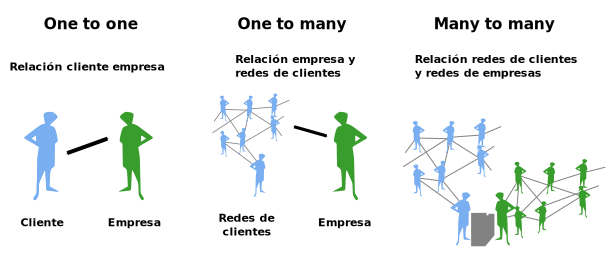
\includegraphics[width=150mm]{capitulos/graficos/oneMany} 
	\label{fig:oneMany} 
	
		\footnotesize
		Fuente: Adaptado de Gummensson, 2004, p. 3.
\end{figure}

En cambio, Prahalad y Ramaswamy (2004), Blasco, (2014) y Gummensson (2004), establecen una escala con tres niveles, dependiendo del número de clientes y la complejidad de la interacción entre la/s empresa/s y el/los cliente/s. En la figura  \ref{fig:oneMany}, se puede apreciar la evolución de estas relaciones surgidas a lo largo del siglo XX (Gummensson, 2004) que son las siguientes:

\begin{itemize}
	\item \emph{One to one} o interacción entre la empresa y el cliente. La contribución \emph{one to one} es la más tratada en la literatura ya que es la forma más sencilla de arrojar luz sobre la interacción individual en la comercialización (Gummensson, 2004).


	\item \emph{One to many} o interacciones entre la empresa y comunidades de clientes. Es un proceso, mediante el cual la empresa transmite informaciones, contenidos, sugerencias, etc. También se puede dar el caso de que la empresa permita interactuar a las comunidades de consumidores entre si (Hoffman y Novak, 1995). Además, la heterogeneidad de los clientes hace que la empresa tenga que adaptarse al amplio abanico de reacciones de estos. Y por lo tanto, la compañía tiene que tener en cuenta que se pueden dar numerosos casos distintos de co-creación de valor (Gummensson, 2004).

 	\item \emph{Many to many} o interacciones llevadas a cabo entre redes de empresas y comunidades de consumidores. La contribución de \emph{many to many} es la más compleja y aborda todo el contexto de un modelo mucho más complejo . Surgió en el año 2000 con el objetivo de describir, analizar y utilizar las propiedades de las nuevas redes de comercialización para poder dar un carácter personalista y poder co-crear valor a través de la interacción (Gummensson, 2004).

\end{itemize}


 Las dos relaciones más comunes de las tres mencionadas anteriormente según Gummensson (2004), son \emph{one to one} y \emph{many to many}. En el cuadro \ref{tab:diferencias} se pueden apreciar algunas de las diferencias entre estas dos propuestas.

\begin{table}[h]
    \caption {Diferencias entre one to one y many to many}
	\label{tab:diferencias}
	\setlength\extrarowheight{5pt}
	
	\begin{tabular}{p{7cm} p{7.5cm}}
	\toprule
	One to one                                           & Many to many                                                                             \\ 
\midrule
	La empresa identifica al consumidor.                 & Las redes de empresas identifican a las redes de consumidores.                           \\
	La empresa diferencia a un consumidor de otro.       & Las redes de empresas se diferencian a través de sus propias relaciones.                 \\
	La empresa interactua con el consumidor.             & Las redes de empresas interactúan con las redes de consumidores a través de otras redes. \\
	La empresa aprende a relacionarse con su consumidor. & Las redes de empresas aprenden a relacionarse a través de redes.                         \\ 
	\bottomrule
	\end{tabular}

	\center
	\footnotesize
	Fuente: adaptado de Gummensson, 2004. p: 3
\end{table}


 Por lo tanto, se puede decir que \emph{one to one} tan sólo abarca la relación individual de una transacción entre una única empresa y un único cliente y en cambio, \emph{many to many} es mucho más compleja y trata de abordar la red de relaciones que tienen las empresas y la red de relaciones que también tienen los consumidores utilizando otra serie de redes para conectar ambas entre si.

Un ejemplo de las redes de relaciones de consumidores son las comunidades Web. En la figura \ref{fig:WomGebauer}, se puede apreciar el modelo conceptual creado por Gebauer, Füller y Pezzei (2013) donde se observa el comportamiento que los usuarios pueden adoptar a la hora de co-crear valor a través de una comunidad Web. Los comportamientos de los clientes pueden ser dos:

\begin{itemize}
	\item \emph{WOM}. Es el boca a boca o también conocido como boca a oreja. Las siglas se corresponden con las palabras inglesas: Word of Mouth.
	\item \emph{WTP}. Son las siglas inglesas \emph{Willingness To Pay}, que se traduce como lo que el cliente está dispuesto a pagar por un producto o servicio.

\end{itemize}

\begin{figure}[!h]
	\caption{El modelo conceptual del comportamiento por parte de los usuarios en las comunidades de innovación online}
	\centering 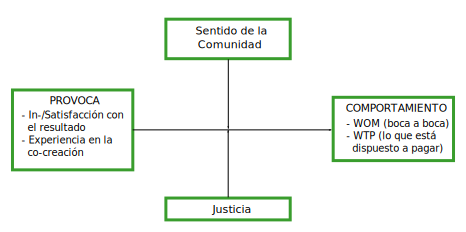
\includegraphics[width=130mm]{capitulos/graficos/WomGebauer} 
	\label{fig:WomGebauer} 
	
		\footnotesize
		Fuente: Gebauer, Füller y Pezzei, 2013, p. 1522.
\end{figure}


Tradicionalmente, se afirmaba que mediante el boca a boca de un consumidor insatisfecho, este usuario transmitía su sentimiento de decepción hacia esa marca a cinco personas de su entorno. Sin embargo, la situación actual es muy diferente, ya que la magnitud es mucho mayor con el desarrollo de las redes sociales (Gebauer, Füller y Pezzei, 2013). Un claro ejemplo es Facebook, esta red social tiene una media mensual de un billón de usuarios activos que a su vez están conectados a 130 amigos de media (Facebook, 2014). Por lo tanto, las opiniones publicadas en las redes sociales, que pueden estar abiertas al público y no sólo al círculo cercano del usuario, tienen un efecto boca a boca mucho más potente y trascendente que en el propio medio social del individuo. Por lo tanto, la co-creación de valor, no siempre es positiva y se puede dar el caso de que la co-creación de valor sea negativa. Se puede encontrar más información respecto a este tema en el anexo \ref{anexo:2}.

En lo que se refiere al proceso de co-creación de valor entre las empresas y los clientes, Yi y Gong (2012) proponen ocho pasos en el sector servicios. A continuación se exponen junto con un ejemplo del sector hotelero:

\begin{enumerate}
	\item \emph{La búsqueda de información}. El huésped potencial puede revisar opiniones de otros huéspedes a través de Tripadvisor.
	\item \emph{El intercambio de información}. El huésped puede reportar problemas al hotel y puede comunicar a otros clientes si se solucionaron con eficacia o no.
	\item \emph{El comportamiento responsable}. Seguir las indicaciones del personal de cocina a la hora del desayuno, comida o cena.
	\item \emph{La interacción personal}. Los empleados deben de adoptar una postura de respeto permanente hacia el cliente.
	\item \emph{Feedback de los clientes}. Los huéspedes deben reportar siempre cualquier problema surgido a lo largo de la estancia y posteriormente pueden realizar una encuesta de calidad para dar una valoración del hotel.
	\item \emph{Promoción}. Es muy importante que los clientes queden satisfechos para que puedan promocionar y recomendar la empresa a desconocidos, familiares y amigos. Es una herramienta de marketing muy importante como se ha podido apreciar en la figura \ref{fig:WomGebauer}, por lo que hay que promover la satisfacción de los clientes.
	\item \emph{Ayuda}. Las opiniones de los huéspedes son muy valiosas para la compañía hotelera porque les ayuda a integrar nuevas herramientas de co-creación de valor en un futuro.
	\item \emph{Tolerancia}. Durante el check in y el check out pueden surgir problemas informáticos, en la gestión de cobros, etc. y el huésped ha de aprender a ser paciente.

\end{enumerate}


Por lo tanto, Yi y Gong (2012) dan importancia a la conducta que adquieren los clientes. Los procesos de co-creación de valor, deben ayudar a los directivos a la hora de elegir nichos de mercado. De este modo, si una empresa evalúa periódicamente las actividades que desarrollan los clientes dentro de la corporación, éstos estarán a su vez más dispuestos a involucrarse en eventos propuestos por la empresa para la co-creación de valor y por lo tanto podrán fidelizarse con la compañía.

\section{Los procesos de co-creación de valor}
\label{section:procesosCocreacion}

A lo largo de literatura dedicada al proceso de co-creación de valor, los autores han decidido centrarse en mayor medida en la relación entre cliente y empresa. Dentro de esta vertiente, Blasco (2014) diferencia dos enfoques: 

\begin{itemize}
	\item Los procesos de co-creación de valor que se pueden dar entre empresa y cliente (Prahalad y Ramaswamy, 2004; Payne et al., 2008), y 
	\item Los procesos de co-creación de valor como una oportunidad de desarrollo de nuevos productos y/o servicios (O’hern y Rindfleisch, 2010). 

\end{itemize}

Los procesos de co-creación de valor como una oportunidad de desarrollo de nuevos productos y/o servicios, dada su poca relación con el objetivo del trabajo no se va a desarrollar en el presente capítulo; se puede encontrar información al respecto en el anexo \ref{anexo:3}. 
A continuación se va a arrojar luz acerca de la co-creación de valor desde el punto de vista del intercambio de información entre la empresa y el cliente. 

\subsection{La participación de la empresa y el cliente en el proceso de creación de valor}

Es destacable que a la hora de producir un servicio se distingan tres formas dependiendo del grado de participación que se le permita al consumidor (Blasco, 2014) (ver figura \ref{fig:procesosCocreacionPayne}):

\begin{itemize} 
	\item Producción completa de la empresa. 
	\item Producción conjunta (relación empresa-cliente). 
	\item Producción del cliente. 
\end{itemize}


\begin{figure}[!h]
	\caption{El proceso de co-creación de valor cliente-empresa}
	\centering 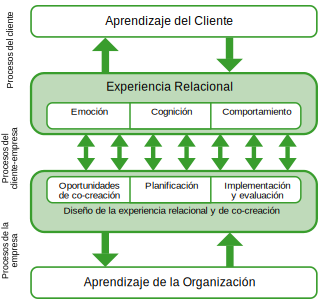
\includegraphics[width=100mm]{capitulos/graficos/procesosCocreacionPayne} 
	\label{fig:procesosCocreacionPayne} 
	
		\footnotesize
		Fuente: Payne, Storbacka y Frow, 2008, p. 96.
\end{figure}

Payne et al. (2008), definen el proceso de creación de valor del cliente como una serie de actividades llevadas a cabo por el usuario para lograr un objetivo particular. El aspecto clave para estos autores, es que la capacidad del cliente para co-crear valor depende de la cantidad de información, de los conocimientos, de las habilidades y de otros recursos operantes que pueden utilizar. Si una empresa quiere mejorar su competitividad, tiene que desarrollar su capacidad y utilizar los recursos de los que dispone de la manera más eficiente y eficaz. Estos autores diferencian tres tipos de etapas a lo largo de este proceso (ver figura \ref{fig:procesosCocreacionPayne}) que se van a explicar a continuación (Payne et al., 2008):


\begin{enumerate} 
	\item \emph{El proceso de co-creación de valor para el cliente}. Los clientes están involucrados en un proceso cognitivo donde realizan juicios en base a sus experiencias de consumo, es decir, a partir de las emociones, de los aspectos contextuales, simbólicos y no utilitarios del propio consumo. En este enfoque, se espera que el cliente esté dispuesto a obtener el conocimiento suficiente para evaluar los beneficios y los sacrificios que conllevan la adquisición del producto o el disfrute del servicio. Si el cliente acepta este reto, las actividades que se han de llevar a cabo son: la búsqueda de información, la evaluación de opciones disponibles y decidir si debe o no comprar un producto o servicio en particular (Payne et al., 2008). Desde este enfoque, se considera que el valor no reside en el momento de la compra o disfrute del bien o servicio, sino en la experiencia de consumo a través de fantasías, sentimientos y diversión. De este modo, Payne et al. (2008), consideran a los clientes como \emph{hacedores y pensadores} de co-creación de valor (ver figura \ref{fig:procesosCocreacionPayne}).
	\item \emph{El proceso de co-creación de valor para la empresa}. Se ha de tener en cuenta el punto anteriormente descrito ya que los clientes crean valor con el apoyo de la empresa. En la figura \ref{fig:procesosCocreacionPayne} se puede apreciar que la empresa participa en la co-creación de valor a través del diseño y la entrega de experiencias al cliente facilitando a su vez el aprendizaje de la compañía. Según Payne et al. (2008), esto implica revisar constantemente las oportunidades que la compañía ofrece a la hora de co-crear, planificar, dar soluciones a los clientes, gestionar los recursos humanos de los que se dispondrán y poner a prueba las medidas diseñadas para los clientes por si no se se están realizando las propuestas de valor adecuadas. Por lo que, partiendo de los procesos de aprendizaje del cliente, una empresa puede diseñar sus propios procesos para aproximarse cada vez más a los de sus clientes. La implementación de este proceso puede desembocar en mejores oportunidades en el proceso de co-creación de valor. 
	\item \emph{El proceso de co-creación de valor entre empresa y cliente}. Se trata de interacciones bidireccionales que se dan entre el cliente y la empresa. Payne et al. (2008) las denomina puntos de contacto. Pueden darse por iniciativa de la propia empresa o por parte del cliente. En la figura \ref{fig:procesosCocreacionPayne}, las interacciones están representadas a través de las flechas situadas entre el cliente y la empresa. Un ejemplo aplicado a la parte empírica expuesta en el capítulo \ref{section:parteEmpirica}, podría ser una campaña de marketing por parte del la empresa hotelera ofreciendo estancias en hoteles a precios reducidos. En algunos casos, la comunicación puede darse por una parte, por ejemplo gracias al envío de publicidad del hotel a los huéspedes fidelizados. Aun así, Payne et al. (2008) opina que ambas partes participan en el proceso porque que la lógica del servicio (Grönrros, 2004) apoya la teoría de que el diálogo es creciente entre ambas partes.

\end{enumerate}

Para finalizar con este epígrafe centrado en los procesos de co-creación de valor, se va a presentar la figura \ref{fig:metasMaram} donde se puede apreciar las relaciones que tanto empresa como cliente han de desarrollar en los procesos productivos para alcanzar la meta de la co-creación de valor y poder obtener clientes fieles, que se impliquen en las tareas de marketing y publicidad a través del boca a boca (Maram, 2013).

\begin{figure}[!h]
	\caption{Pasos para alcanzar la co-creación de valor}
	\centering 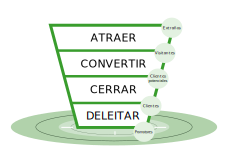
\includegraphics[width=110mm]{capitulos/graficos/metasMaram} 
	\label{fig:metasMaram} 
	
		\footnotesize
		Fuente: Maram, 2013
\end{figure}

\section{Las teorías asociadas a la co-creación de valor}

En el presente epígrafe, se van a describir las principales teorías surgidas sobre la co-creación de valor desarrolladas hasta el momento. En la figura \ref{fig:esquema} se aprecia un esquema de las tres diferentes ramas que se van a asumir acerca de la co-creación de valor y los autores creadores o defensores de éstas. Se va a seguir el modelo de segregación en tres vertientes de los autores Chen et al. (2012).

\begin{figure}[!h]
	\caption{Esquema de las teorías de co-creación de valor}
	\centering 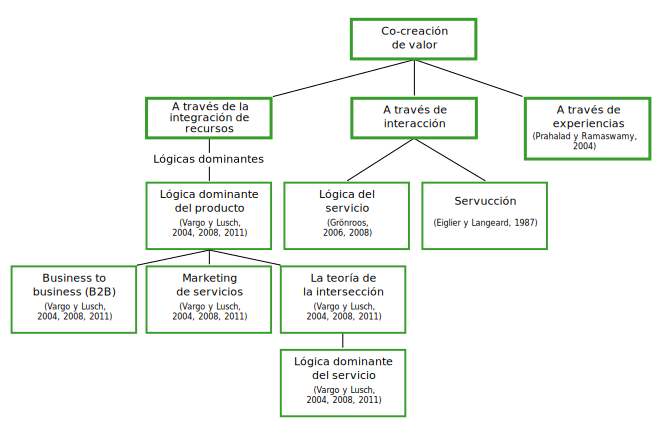
\includegraphics[width=150mm]{capitulos/graficos/esquema} 
	\label{fig:esquema} 
	
		\footnotesize
		Fuente: elaboración propia
\end{figure}

Como se puede apreciar en la figura \ref{fig:esquema}, Vargo y Lusch son defensores de la lógica dominante del servicio que parte de las premisas de la lógica dominante del producto; Grönroos apoya la lógica del servicio; Eigler y Langeard desarrollan la teoría de la servucción; y por último, Prahalad y Ramaswamy defienden las relaciones personalizadas entre empresa y cliente para que éste último pueda interaccionar con el entorno empresarial y crear experiencias personalizadas. 

\subsection{La co-creación de valor a partir de la integración de recursos}

\subsubsection{Las lógicas dominantes}

El término de lógica dominante hace referencia a las pautas que desarrolla una empresa para obtener beneficios. En la lógica dominante se describen las normas y las creencias culturales que la empresa ha desarrollado en su camino al éxito o al fracaso. Aitken, et. al. (2006) definen la lógica dominante como un pensamiento común basado en las estrategias de diferentes empresas.

\paragraph{De la lógica dominante del producto a la lógica dominante del servicio}
\label{section:logicasDominantes}

La lógica dominante del producto (LDP), no distingue entre bienes tangibles e intangibles y su esencia es el intercambio económico de unidades de producción que tienen el valor intrínseco en si mismo. La producción y el desarrollo del bien se realiza sin el cliente (Vargo y Lusch, 2008). La figura \ref{fig:valorUso} refleja estas diferencias marcadas por Vargo y Lusch (2004) entre el proceso de co-creación de valor en el intercambio (LDP) y el proceso de co-creación de valor en el uso (LDS). En este último, la variable más trascendente es la experiencia de valor acumulada en uso por parte del cliente, ya que en este modelo, el cliente tiene que participar en el proceso de co-creación de valor. 

\begin{figure}[!h]
	\caption{Comparación del proceso de co-creación en el modelo de valor en el intercambio y en el modelo de valor en uso}
	\centering 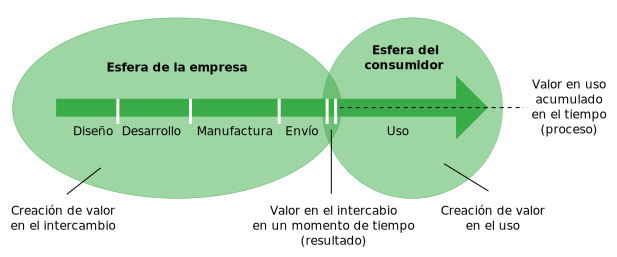
\includegraphics[width=150mm]{capitulos/graficos/valorUso} 
	\label{fig:valorUso} 
	
		\footnotesize
		Fuente: Grönroos y Voima, 2011, p. 4.
\end{figure}

Para poder comprender esta evolución de teorías, en la figura \ref{fig:evolucion} se van a delimitar las fechas en las que surgen cada una de las teorías. Los tres enfoques surgidos a partir de la LDP, son conceptos definidos en el anexo \ref{anexo:4}.

\begin{figure}[!h]
	\caption{Evolución de la lógica dominante}
	\centering 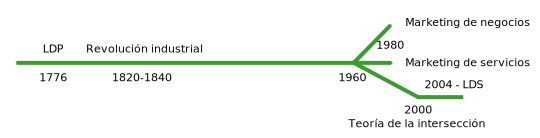
\includegraphics[width=150mm]{capitulos/graficos/evolucion} 
	\label{fig:evolucion} 
	
		\footnotesize
		Fuente: elaboración propia a partir de Vargo y Lusch, 2008
\end{figure}

Como se puede observar en la figura \ref{fig:evolucion}, el concepto lógica dominante del servicio (LDS) surge por primera vez en la obra de Smith del año 1776, se desarrolló a lo largo de un siglo atravesando también la revolución industrial y llegó hasta los años 60 acumulando un amplio conocimiento acerca de la economía (Vargo y Lusch, 2008). Desde las raíces de esta teoría, se consideró que la empresa creaba un producto con un valor añadido intrínseco y el cliente destruía ese valor a través del consumo. Pero como bien se ha mencionado, a partir de 1960 la mentalidad empresarial sufrió un cambio y esta teoría comenzó a ser cuestionada, dando lugar a la creación de subdisciplinas. El nacimiento de éstas se debe a la limitación de la LDP para dar respuesta a la creación de valor y al intercambio entre otros factores, ya que la LDP solo se refiere a la distribución de productos (Vargo y Lusch, 2008).


A continuación, se van a exponer las características más importantes de la lógica dominante del servicio (LDS) y de la lógica dominante del producto (LDP). Se explican al mismo tiempo ya que Vargo y Lusch (2004) las tratan conjuntamente.

Se puede afirmar que la LDS surgió de las limitaciones que la LDP tenía para el concepto de servicio. Tanto Vargo y Lusch (2004), como Grönroos  (2006), coinciden en que los servicios también forman parte de la teoría de la lógica dominante del producto de una forma secundaria, pero para poder abarcar más elementos Vargo y Lusch (2004) crearon la lógica dominante del servicio. Esta nueva rama, abarcaba conceptos de procesos de comercialización para la empresa que la LDP no contemplaba tales como las relaciones a largo plazo, la calidad percibida por el cliente, las relaciones entre usuario y empresa, la transparencia, los enfoques hacia el intercambio y la sostenibilidad entre otros. Estos nuevos conceptos incluidos en la LDS, permitieron a Vargo y Lusch, desarrollar este nuevo modelo con variaciones en la forma de crear valor y la forma de intercambiar el servicio, como por ejemplo la calidad percibida y los recursos humanos dispuestos por la empresa. 

Según establecen Vargo y Lusch, (2011) la lógica dominante del servicio es una lógica \emph{de y para} el mercado, la sociedad y la comercialización. Esta nueva concepción centrada en el servicio, se ve reflejada en que la co-creación de valor es la integración de valor en el propio contexto teniendo en cuenta los resultados y los recursos de la empresa. Por ejemplo, como un huésped utiliza los recursos disponibles del hotel (Vargo y Lusch, 2008). Por lo tanto, estos autores establecen que la integración predeterminada de recursos en un proceso co-creativo es un medio de creación de valor.

Otro de los obstáculos de la LDP era el léxico. La primera columna del cuadro \ref{tab:evolucionLexica} está referida a la LDP, y se trata de un léxico basado en la economía de la primera década de 1800 que fue aceptado y utilizado al menos hasta aproximadamente el año 1980. Alrededor de 1980, surgió una grieta en el léxico provocada por una transición de la comercialización del servicio al marketing relacional y los recursos de intercambio y competencia, entre otros (Vargo y Lusch, 2004). Algunas de estas palabras llevan connotaciones muy específicas y se encuentran encasilladas en una lógica concreta y a menudo son incompatibles (Vargo y Lusch, 2004). Por ejemplo, productor y consumidor; bienes y servicios; demanda y oferta; etc. El léxico que surge para la LDS es más cercano y agradable para el cliente como por ejemplo los términos diálogo, proposiciones de valor, soluciones, etc. Vargo y Lusch (2004) afirman que todavía no se ha desarrollado plenamente todo el léxico que se debería para la LDS, por ello, plantean seguir desarrollando la LDS. 

\begin{table}[h]
    \caption {Evolución del léxico en las lógicas dominantes}
	\label{tab:evolucionLexica}
	\setlength\extrarowheight{5pt}
	
	\begin{tabular}{p{5cm} p{5cm} p{5cm}}
	\toprule
	LDP                               & Transición                            & LDS                              \\ \midrule
	Bienes                            & Servicios                             & Servicio                         \\
	Productos                         & Ofertas                               & Experiencias                     \\
	Características/atributos         & Beneficio                             & Soluciones                       \\
	Valos añadido                     & Co-producción                         & Co-creación de valor             \\
	Beneficio máximo                  & Ingeniería financiera                 & Aprendizaje financiero           \\
	Precio                            & Entrega de valor                      & Proposición de valor             \\
	Sistemas de equilibrio            & Sistemas dinámicos                    & Sistemas complejos de adaptación \\
	Red de creación de valor          & Cadena de valor                       & Red de co-creación de valor      \\
	Fomento                           & Marketing de comunicaciones integrado &                                  \\
		                              &                                       & Diálogo                          \\
	Mercado orientado a los productos & Mercado orientado al mercado          & Mercado orientado al servicio    \\ \bottomrule
	\end{tabular}
	
	\center
	\footnotesize
	Fuente: Vargo y Lusch, 2004. p. 286
\end{table}


Esta evolución lingüística también afecta a la forma de entender la co-creación de valor. Por ello, Vargo y Lusch (2008) establecen tres importantes diferencias:

\begin{enumerate} 
	\item La LDP afirma que el valor de bienes y servicios está intrínseco en el propio bien. En cambio, la LDS considera que el servicio es el proceso por el que la empresa hace algo para el cliente sin hacer referencia a los bienes que intervienen en el intercambio. Esto quiere decir que en la LDS los bienes siguen teniendo un papel importante aunque no sean mencionados (Vargo y Lusch, 2008). 
	\item El tratamiento de los elementos. La LDP, considera que los servicios tienen una categoría inferior a la de los bienes fabricados, y la LDS, en cuanto a la co-creación de valor, considera que es un proceso relacional de intercambio de servicio por servicio. Este intercambio, implica que tanto empresa como cliente son co-creadores y beneficiarios de valor, y deben considerarse como integradores de recursos (Vargo y Lusch, 2011). 
	\item La diferencia de léxico entre servicios y servicio: 
		\begin{itemize} 
			\item Los servicios. Son unidades de \emph{output} (Vargo y Lusch, 2004). Para Grönroos (2004), son procesos de una serie de actividades en las que la empresa utiliza unos recursos determinados cuando interacciona con el cliente. Se relaciona con la LDP.
			\item El servicio. Se trata de un proceso de \emph{algo para alguien} (Vargo y Lusch, 2004). Se relaciona con la LDS.

			De este modo, el uso del término servicio en singular en contra a los servicios que plantea la LDP, es intencional y no trivial (Vargo y Lusch, 2008). Para Vargo y Lusch (2004) uno de los errores fundamentales de la LDP es que el servicio es considerado como un tipo especial de bien intangible.
			\end{itemize}

\end{enumerate}

Por otro lado, en la LDS el proceso de co-creación de valor recíproco es un proceso continuo de integración de recursos que pueden ser de dos tipos (Vargo y Lusch, 2006):

\begin{itemize} 
			\item Los recursos operandos. Vargo y Lusch (2008) los definen como los recursos sobre los cuales se realiza una operación o un acto para producir un efecto, es decir, se trata de recursos estáticos e inertes que necesitan de otros recursos dinámicos para que sean útiles. Algunos ejemplos son los recursos naturales, bienes, materiales tangibles, etc. (Vargo y Lusch, 2008).
			\item Los recursos operantes o dotación de recursos. Son los recursos capaces de afectar sobre los recursos operandos ya que se refieren a las habilidades, el conocimiento, la imaginación, las emociones y las experiencias de los clientes. Por lo tanto, estos recursos también afectan a la co-creación de valor. Se puede ampliar el modelo co-creativo incluyendo las interacciones entre empresas, clientes y \emph{stakeholders} (Vargo y Lusch, 2011). Como conclusión, Vargo y Lusch (2008) establecen que todo el entorno social y económico integra recursos de un tipo u otro.

\end{itemize}

Teniendo en cuenta la integración de recursos mencionada en el párrafo anterior, se puede observar la figura \ref{fig:LDSVargoLusch} que refleja el proceso de co-creación de valor en la lógica dominante del servicio. En ella se muestra cómo interaccionan los clientes con la empresa mediante los recursos internos y externos que se proporcionan, teniendo en cuenta también los agentes que podrían considerarse como resistencias a la co-creación de valor. Hasta que estas resistencias u obstáculos sean superados e integrados por la empresa, se continuará utilizando el mismo sistema de interacción entre el cliente y la empresa para co-crear valor (Lusch y Vargo, 2007).

\begin{figure}[!h]
	\caption{El proceso de co-creación de valor en la lógica dominante de los servicios}
	\centering 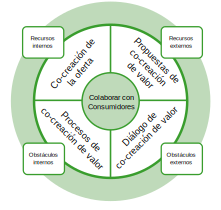
\includegraphics[width=100mm]{capitulos/graficos/LDSVargoLusch} 
	\label{fig:LDSVargoLusch} 

	\footnotesize
		Fuente: Vargo y Lusch, 2008, p. 4.
\end{figure}

En resumen, el paso natural de la LDP hacia la LDS propone los siguientes cambios (Vargo y Lusch, 2008) (ver cuadro \ref{tab:transicion}): 

\begin{enumerate} 
			\item Del pensamiento de producción de bienes y servicios a un proceso de ayuda al cliente para facilitar el desarrollo de la co-creación de valor. 
			\item Concebir el valor como un bien producido y vendido a verlo como una variable co-creada en conjunto con el cliente y el entorno. 
			\item Considerar al cliente como parte de la empresa y no como un ente aislado.
			\item Incluir los recursos operantes intangibles como el conocimiento y las habilidades a los recursos operandos de la empresa como pueden ser los recursos naturales. 
			\item Concebir a los clientes como fuente de información y recursos. 
			\item El cambio de mentalidad de que prime la eficiencia a que aumente esa eficiencia a través de la eficacia. 

\end{enumerate}

\begin{table}[h]
    \caption {Transición de la LDP a la LDS.}
	\label{tab:transicion}
	\setlength\extrarowheight{5pt}
	
	\begin{tabular}{p{7cm} p{7.5cm}}
	\toprule
	LDP                                                      & LDS                                                                          \\ \midrule
	Producir bienes o servicios.                             & Ayudar a los clientes en los procesos de co-creación de valor.               \\
	El valor se halla en los bienes o servicios producidos.  & Los clientes no son entidades aisladas si no que forman parte de la empresa. \\
	Los recursos principales de la empresa son los operandos. & Los recursos principales de la empresa son los operantes.                    \\
	Los clientes son el objetivo.                            & Los clientes son recursos.                                                   \\
	Prima la eficiencia.                                     & Prima la eficiencia a través de la eficacia.                                 \\ \bottomrule
	\end{tabular}

	\center
	\footnotesize
	Fuente: Vargo y Lusch, 2008. p. 5.
\end{table}


Estos cambios implican una remodelación de valores empresariales que facilitan la co-creación de valor conjuntamente. Es decir, se trata de un intercambio entre empresa, cliente y entorno. 

Como conclusión, se puede afirmar que el fin de la LDP es la reciprocidad, es decir, el momento en el que se presta el servicio ha de hacerse \emph{para y con el cliente} con el objetivo de obtener un intercambio de servicio por servicio.  Los productos pueden aparecer en este intercambio pero como complementos y en segundo plano. Los elementos participantes fundamentales son el conocimiento y las habilidades que la compañía emplea para la creación de valor (Vargo y Lusch, 2004). Por tanto, queda patente que en la teoría de la LDS, la co-creación de valor se centra en el hecho de que el cliente siempre participa activamente en el proceso de co-creación de valor, implicándose hasta tal punto de emplear sus propios recursos operantes además de aprovechar los recursos facilitados por la empresa (Vargo et al., 2010). En estudios paralelos de Vargo, Maglio y Akaka (2008) se propone la co-creación de valor como un proceso más complejo en el que se incluyen agentes como los \emph{stakeholders}, agencias gubernamentales, etc. No se va a entrar en más detalle por la complejidad que supone este modelo.

\subsection{La co-creación de valor a través de la interacción}

En este epígrafe se van a explicar dos teorías que defienden que el intercambio de valor se produce en el momento en el que la empresa y el cliente interaccionan entre sí, por ello, la empresa debe procurar instaurar sistemas que permitan estas interacciones. Las dos teorías más relevantes de co-creación de valor a través de la interacción son (Blasco, 2014):

\begin{itemize} 
    \item El modelo de servucción (Eiglier y Langeard, 1975, 1976). 
    \item La lógica del servicio (Grönroos, 2006, 2008). 
\end{itemize}

Como se puede apreciar en la figura \ref{fig:procesoProductivoEiglier}, la diferencia fundamental entre la producción de productos y la producción de servicios está en que en el \emph{input} existen otros elementos. En los servicios, el cliente es simultáneamente el productor y el consumidor, es decir, la entrada y la salida del proceso productivo es el cliente. Esto ocurre porque el consumidor es quien ha disfrutado del servicio y ha sido al mismo tiempo co-productor. En cambio, en la producción de un bien tangible, existe una transformación de recursos y por lo tanto, el \emph{input} y el \emph{output} son diferentes. Por ello, es necesario incorporar esta herramienta de diseño de servicios, al departamento de calidad de empresas dedicadas a los servicios (Eiglier y Langeard, 1976). 

\begin{figure}[!h]
	\caption{Diferencias en el proceso productivo del servicio y del producto}
	\centering 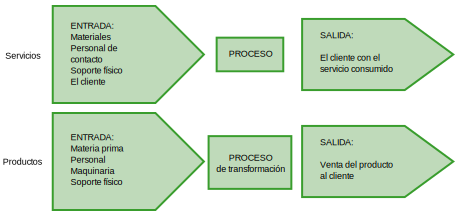
\includegraphics[width=150mm]{capitulos/graficos/procesoProductivoEiglier} 
	\label{fig:procesoProductivoEiglier} 

	\footnotesize
		Fuente: Adaptado de Lilian, 2004, p. 5.
\end{figure}

En primer lugar, se describirá la teoría de Eigler y Langeard diseñada en los años 80. Y en segundo lugar, la teoría desarrollada por la escuela nórdica, más concretamente por Grönroos sobre la lógica del servicio y el marketing interactivo que se ha creado en la primera década del año 2000.

\subsubsection{La servucción}

Eiglier y Langeard, (1976) definen servucción como la organización sistemática y coherente de todos los elementos físicos y humanos que surgen de la relación entre el cliente y la empresa y que es necesaria en la prestación de servicios, donde las características comerciales y los niveles de calidad que se van a ofrecer han sido determinados por la empresa.

Cuando la empresa establece su plan de prestación de servicios, tiene que tener una serie de factores que van a influir en este proceso y que han de desarrollarlos con sumo cuidado. Por ejemplo, la gestión de los procesos de trabajo, las capacidades personales, el flujo de clientes, etc. Puede considerarse un reto para la empresa ya que pone de manifiesto la creatividad y a la precisión de la que disponen, teniendo en cuenta todos los elementos subjetivos que se pueden dar en el comportamiento del cliente. Por ejemplo, las relaciones establecidas con el personal prestador del servicio, las expectativas, los deseos, las variaciones y las percepciones decisivas del cliente, etc. Hay que tener en cuenta un aspecto fundamental, y es que \emph{sin cliente no existe el servicio} (Eiglier y Langeard, 1976). Por ejemplo, si el cliente no ocupa la habitación de un hotel solo se daría la capacidad ociosa de servicio, pero no el servicio en si. 

\begin{figure}[!h]
	\caption{La servucción: empresa, cliente y entorno según Eiglier y Langeard}
	\centering 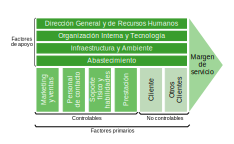
\includegraphics[width=140mm]{capitulos/graficos/servuccion} 
	\label{fig:servuccion} 

	\footnotesize
		Fuente: Alonso, 2008, p. 89.
\end{figure}

A continuación se va a dar sentido a la figura \ref{fig:servuccion} a través de ejemplos para un hotel, que es el tema a tratar en el capítulo \ref{section:parteEmpirica}.

Los factores principales que pueden ser controlables por la empresa son (Eiglier y Langeard, 1976):

\begin{itemize} 
			\item El marketing y las ventas. No se da con frecuencia, pero algunos ejemplos son: promocionar un nuevo alimento en el desayuno, una ropa de cama más confortable, etc. 
			\item El personal de contacto en el momento del servicio. El personal deberá de procurar que el check in y el check out se desarrollen sin incidencias. O por otro lado, si el cliente percibe algún problema lo reporte y se resuelva amablemente poniendo de manifiesto los valores del hotel. 
			\item El soporte físico y las habilidades. La sociedad actual se encuentra muy concienciada en la práctica de deporte, por ello, los hoteles poco a poco van incorporando salas de gimnasio gratuitos para sus huéspedes, piscinas, spas, salas de masaje, etc. 

\end{itemize}

En segundo lugar, se pondrán ejemplos para las variables clientes y otros clientes que pueden participar a la hora de producirse el servicio (Eiglier y Langeard, 1976) (ver figura \ref{fig:servuccion}):

\begin{itemize} 
			\item El cliente. Influye también el conocimiento previo que haya adquirido en otras experiencias en hoteles o incluso en la vida cotidiana. Si el cliente acepta participar en el proceso de co-creación, serán de vital importancia para la empresa las relaciones y las conversaciones con el personal del hotel. Si por el contrario, el cliente no acepta participar, el hotel deberá de haberlo previsto y deberá minimizar los desvíos de conducta del huésped para que afecte en menor medida a la hora del disfrute del servicio. 
			\item Otros clientes. Puede darse el caso de que varios huéspedes coincidan y conversen en la recepción del hotel, en el bar o en el gimnasio. 

\end{itemize}

En tercer lugar, se exponen los factores complementarios y sus correspondientes ejemplos (Eiglier y Langeard, 1976):

\begin{itemize} 
			\item La dirección general y de recursos humanos. Cada uno de los empleados deben ser formados por la cadena hotelera para asumir los valores de la empresa y comunicarlos a los clientes además de diseñar un conjunto de estrategias para que el servicio se lleve a cabo de la manera más eficiente y eficaz teniendo en cuenta las exigencias más recientes de los mercados y de los clientes 
			\item La organización interna y la tecnología. Es el conjunto de funciones que los diferentes departamentos tienen que desempeñar ayudados por los avances tecnológicos de los que la empresa disponga para facilitar la prestación del servicio, los procesos de investigación de mercados, el desarrollo de nuevos conceptos, etc. La organización interna debe vigilar su realización de forma coherente, consistente, homogénea y coordinada. 
			\item La estructura y el ambiente. Son el mantenimiento del hotel, la atmósfera que se crea con la música y los olores, la limpieza, la decoración, etc. 
			\item El abastecimiento. Se trata de la adquisición de materiales, insumos, soportes físicos, servicios de capacitación, publicidad, seguros de salud, y todos los demás elementos indispensables para la prestación del servicio. 
\end{itemize}

\begin{figure}[!h]
	\caption{El proceso productivo en una empresa de servicios}
	\centering 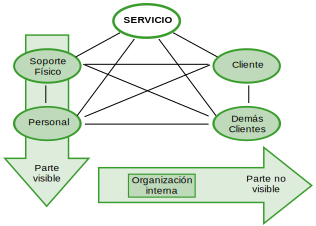
\includegraphics[width=92mm]{capitulos/graficos/procesoProductivoServiciosEiglier} 
	\label{fig:procesoProductivoServiciosEiglier} 

	\footnotesize
		Fuente: Lilian, 2004, p. 6.
\end{figure}

Y por último, hay que mencionar el margen del servicio (Eiglier y Langeard, 1976) (ver figura \ref{fig:servuccion}), que es donde confluyen todos los factores anteriormente definidos una vez que el servicio se ha desarrollado. Se trata de la suma de las ventajas competitivas conseguidas por cada factor por separado. Esto quiere decir, que el resultado del margen es lo que el cliente ha percibido, le ha gustado y ha experimentado, es decir, el vínculo real y emocional que se ha desarrollado dentro del cliente y que ha provocado una fidelización. Por ejemplo, los clientes que pertenecen al club de fidelidad que el hotel del estudio empírico propone y en el cual, se reciben descuentos, estancias en hoteles gratuitas, etc.

A modo de resumen, Eiglier y Langeard, (1976) plantean un  proceso productivo en los servicios similar al de Grönroos (2004), pero más general ya que fue desarrollado varios años antes (ver figura \ref{fig:procesoProductivoServiciosEiglier}).

Eiglier y Langeard, (1976), establecen tres tipos de ventajas competitivas: 

\begin{itemize} 
			\item La ventaja competitiva enfocada hacia la oferta total del servicio. Para poder alcanzar esta co-creación de valor deben satisfacerse las necesidades de los clientes y del personal, de los proveedores, y de todos los agentes que se encuentren implicados en la toma de decisiones como los \emph{stakeholders}. 
			\item La ventaja competitiva enfocada hacia el soporte de la oferta. Como por ejemplo, el soporte físico, el personal, la organización y la administración. 
			\item La ventaja competitiva enfocada hacia la oferta total del servicio y hacia el soporte de la oferta. Se tienen en cuenta las percepciones de antiguos clientes y en base a sus expectativas, se evalúan, aceptan e integran en el proceso productivo del servicio. Esto pone de manifiesto que el servicio global debe enfocarse a cada segmento de clientes, es decir a los denominados \emph{clientes meta}. 

\end{itemize}

En el desarrollo de los procesos de servucción, no hay que perder de vista que el cliente es la razón de ser del servicio y que las necesidades y la personalidad de los usuarios están en continua evolución, además de la heterogeneidad de cada uno de los clientes. Por lo tanto, la implementación de procesos se encuentra en cambio constante y esto supone un control y una evaluación continuada de los consumidores (Eiglier y Langeard, 1976).

Como conclusión, se puede decir que el análisis de las servucciones permite identificar el soporte físico, el personal que debe ser contratado por la empresa y la organización interna necesaria para satisfacer las expectativas de los usuarios y co-crear valor para el cliente. De este modo, se permite la identificación de aquellas actividades positivas para la empresa, otorgando la oportunidad empresarial de elaborar propuestas de cambio en las actividades conduciendo a una mejora continua de la oferta de servicios satisfaciendo al cliente y alcanzando el objetivo primordial: co-crear valor.

\subsubsection{La lógica del servicio}

La investigación desarrollada por la escuela nórdica se denomina la lógica del servicio (LS) (Grönroos, 2006). Esta corriente de pensamiento sugiere que la creación de valor se basa en la interacción de \emph{servicio por servicio}. Grönroos, argumenta que la interacción de servicio por servicio viene dada por una nueva perspectiva del cliente, mientras que el intercambio de servicios por servicios viene dada por la perspectiva de la empresa.

Por lo tanto, centrándose en la LS, Grönroos (2008) define la interacción como una acción mutua o recíproca en la que el cliente o la empresa tiene efectos uno sobre el otro y viceversa y además, de una forma simultánea, también en los procesos de creación de valor de las empresas. Grönroos, (2008) propone un modelo de productividad para los servicios que se puede visualizar a través de la figura \ref{fig:procesoProductivoServiciosGronroos} y que es más concreto que el de Eiglier y Langeard.

\begin{figure}[!h]
	\caption{El modelo de productividad en los servicios}
	\centering 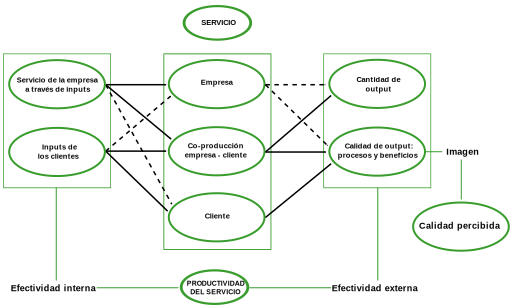
\includegraphics[width=150mm]{capitulos/graficos/procesoProductivoServiciosGronroos} 
	\label{fig:procesoProductivoServiciosGronroos} 

	\footnotesize
		Fuente: Grönroos, 2004, p. 420.
\end{figure}

Grönroos (2008) propone que las interacciones del mercado pueden extenderse más allá de las partes que están en contacto directo entre sí. Incluyendo un nuevo término que es la \emph{facilitación}. Gracias al desarrollo tecnológico existen nuevas formas de interactuar y las empresas deben facilitarlas a los clientes. Estos nuevos métodos de interacción, también influyen en los clientes abarcando novedosos sistemas de co-creación de valor en el que también se integran los recursos. Este punto de vista de que los clientes pueden ser creadores de valor difiere de la visión de la LDS de que los clientes siempre son co-creadores de valor. Como punto común, ambas lógicas reconocen la integración de los recursos como la actividad clave para la creación de valor, pero esta última incluye la interacción. Pero Grönroos (2004), en su postura más radical establece que la integración de los recursos en el proceso de co-creación de valor, puede hacer que los clientes sean los únicos capaces de crear valor. Las empresas podrían participar activamente en los procesos de creación de valor de los clientes y crear valor para los usuarios, y los clientes a su vez crear valor para sí mismos. En el anexo \ref{anexo:5} se puede encontrar más información acerca de esta cuestión.

Otro aspecto importante que resalta Grönroos (2008) en la lógica del servicio, es el cumplimiento de los esfuerzos de los clientes para concretizar y poder hacer realidad el valor. Este cumplimiento del valor es un proceso continuo donde están en juego la actualización y la realización de valor. La actualización es la percepción del cliente a la hora de recibir valor y los esfuerzos que éste emplea para que esa percepción se actualice automáticamente (ver figura \ref{fig:esferasGronroos}).

\begin{figure}[!h]
	\caption{Las esferas de la co-creación de valor en la lógica del servicio}
	\centering 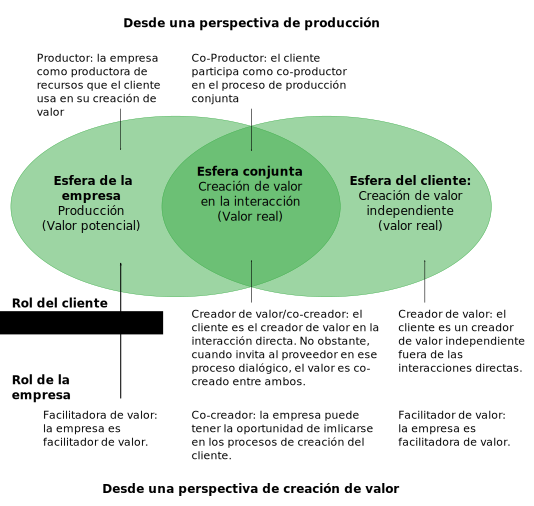
\includegraphics[width=140mm]{capitulos/graficos/esferasGronroos} 
	\label{fig:esferasGronroos} 

	\footnotesize
		Fuente: Grönroos y Voima, 2011 p. 9.
\end{figure}

En la figura \ref{fig:esferasGronroos} se puede observar cómo las funciones de la empresa y cliente varían, dependiendo de la esfera de la co-creación de valor. La empresa es la responsable del proceso de producción donde se producen los recursos y los procesos para el uso de los clientes facilitando así la creación de valor a los usuarios. Tal y como propone Grönroos (2008), si la empresa proporciona un potencial valor en uso, la empresa puede ser considerada como facilitadora de valor. En este caso, el papel del cliente es doble porque es co-creador de valor, y co-productor de los recursos y de los procesos con la empresa porque crean valor de forma conjunta con la compañía. En el momento en el que surge la interacción directa entre la empresa y el cliente, la organización puede tener la oportunidad de participar en un proceso de creación de valor del cliente y asumir el papel de co-creadora de valor. El valor puede surgir también en las otras dos esferas en diferentes períodos de tiempo, formándose así diferentes patrones de creación de valor. Puede darse que un cliente activo sea co-desarrollador o diseñador, o incluso co-fabricante, entonces la esfera conjuntase hace más grande y todo el proceso se iniciadirectamente en la esfera de valor conjunto (Grönroos y Voima, 2011).

En resumen, la lógica del servicio ve la creación de valor como una interacción directa entre los recursos propuestos por la empresa y los recursos propios del cliente y la mezcla de ambos da como resultado la creación de valor. Esta experiencia de interacciones directas hacen posible que tanto empresas como clientes sean capaces de actualizar y darse cuenta de que crean valor. Es importante destacar que este tipo de experiencias pueden ser acumuladas y compartidas en un futuro (Chen et. al., 2012).

\subsection{La co-creación de valor a través de las experiencias}

La tercera perspectiva viene de la mano de Prahalad y Ramaswamy (2004). Estos autores establecen que la co-creación de valor se da en la experiencia de los clientes a la hora del disfrute del bien o servicio, es decir, el valor no deriva del consumo de bienes y servicios, sino que está incrustado en las experiencias personalizadas y reales que se crean gracias al compromiso y la participación conjunta con la empresa. 

Es importante mencionar el momento en el que Prahalad y Ramaswamy (2004) deciden crear una nueva rama, a partir de las teorías desarrolladas hasta el momento, denominada como: la co-creación de valor en las experiencias. En la figura \ref{fig:interaccionPrahalad}, se puede apreciar como las empresas se centran en un modelo de intercambio donde la orientación es hacia el cliente y en el que se incluye este concepto de creación de valor a través de la experiencia del cliente. El valor surge en el momento en el que se produce la interacción y la comunicación entre la empresa y el cliente de una forma personalizada. El mercado es el lugar donde se intercambia el valor y el consumidor tiene que ser persuadido por la empresa para que ésta pueda percibir el máximo valor en el momento de la/s transacción/es. Los clientes están aprendiendo a estar informados, conectados, a ser autorizados por la empresa para poder realizar actividades por si solos y sobre todo a darse cuenta de que ellos también pueden recibir valor, incluso a partir del diálogo de consumidor a consumidor.

\begin{figure}[!h]
	\caption{El proceso de co-creación de valor}
	\centering 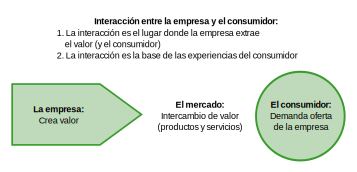
\includegraphics[width=140mm]{capitulos/graficos/interaccionPrahalad} 
	\label{fig:interaccionPrahalad} 

	\footnotesize
		Fuente: Prahalad y Ramaswamy, 2004, p. 7.
\end{figure}

Esta nueva sensación que experimentan los clientes les hace ser conscientes del poder que tienen dentro de una empresa. Por ello, un número cada vez mayor de clientes están mucho más dispuestos a negociar los precios y otras condiciones de transacción con las empresas. Prahalad y Ramaswamy (2004) afirman que la sociedad se está moviendo hacia un mundo en el que el valor es el resultado de una negociación implícita entre el consumidor individual y la empresa. 

Para subsanar el problema de la \emph{walmartización}\footnote{Concepto desarrollado en el anexo \ref{anexo:6}.}, las empresas deben de co-crear valor con los clientes a través de un enfoque obsesivo de interacciones personalizadas entre el consumidor y la empresa. Esto permitirá que los clientes se centren en las experiencias para conseguir co-crear valor. Hay que tener en cuenta el impacto que puede tener la convergencia de ambos ya que en los roles tradicionales son claramente distintos (Prahalad y Ramaswamy, 2004).

En el sistema tradicional, las empresas deciden los productos y los servicios que se producen y qué grado de valor tienen para el cliente, por lo tanto el cliente no co-crea valor. Según los autores Prahalad y Ramaswamy (2004), en las dos últimas décadas las empresas han querido otorgar mayores responsabilidades a los clientes, por ejemplo permitiendo la reserva de habitaciones por Internet. También, los usuarios pueden participar en el diseño de productos. Esto es gracias a que los consumidores están conectados, informados, capacitados y activos continuamente. Por ejemplo, en el sector hotelero existen multitud de establecimientos y algunos de ellos con grandes parecidos, pero lo que les diferencia son las experiencias que proponen al huésped, es decir, la ventaja competitiva a través de la co-creación de valor. Este ejemplo, muestra como los productos o servicios pueden ser de consumo masivo pero por el contrario, las experiencias de co-creación de valor nunca lo pueden ser. 

La co-creación de experiencias se basa principalmente en las interacciones entre la empresa y el cliente mediante el diálogo, el acceso -por ejemplo las plataformas \emph{engagement}-, el riesgo o beneficio compartido y la transparencia (Prahalad y Ramaswamy, 2004). Si se traduce al castellano la palabra \emph{engagement}, se obtendría como resultado: compromiso. Por lo tanto se trata de plataformas de compromiso entre las empresas y los clientes. Estas plataformas puede suponer un punto de contacto visual y físico de integración de recursos y de co-creación de valor. Esto quiere decir, que estas interacciones entre el consumidor y la empresa se pueden convertir en una fuente de resolución de problemas por medio del dialogo, gracias a la rapidez y eficacia del acceso a la información y también a la transparencia. Además, disminuye la incertidumbre y la toma de decisiones es más rápida. Prahalad y Ramaswamy, (2004) desarrollaron esta idea a través del modelo DART: diálogo, acceso, riesgo/beneficio y transparencia (ver figura \ref{fig:DartPrahalad}).

\begin{figure}[!h]
	\caption{El modelo DART para la co-creación de valor}
	\centering \includegraphics[width=90mm]{capitulos/graficos/DartPrahalad} 
	\label{fig:DartPrahalad} 

	\footnotesize
		Fuente: Prahalad y Ramaswamy, 2004, p. 9.
\end{figure}

A continuación, se van a explicar brevemente las variables que componen el modelo DART de Prahalad y Ramaswamy (2004) (ver figura \ref{fig:DartPrahalad}):

\begin{itemize} 
			\item \emph{El diálogo}. Es un elemento muy importante a la hora de la co-creación de valor. Implica la interactividad, la participación, la capacidad y la voluntad de actuación por parte de la empresa y por parte del cliente. Para que sea un un diálogo activo y se desarrolle favorablemente, tanto para la empresa como para el consumidor, ambos deben considerarse como iguales. La base del diálogo es abarcar temas de interés para ambos y no sobrepasar los límites establecidos. 
			\item \emph{El acceso}. Si los si los consumidores no disponen de la misma accesibilidad se vuelve al problema tradicional, donde se experimenta la asimetría de la disposición de información. 
			\item \emph{La transparencia}. Ocurre algo similar a lo explicado en el punto anterior (el acceso). Las empresas tradicionalmente casi siempre se han beneficiado de la explotación de esa asimetría de información que existía entre empresa y consumidor. Actualmente, y gracias a la conectividad, es posible que un consumidor tenga acceso a tanta información como necesite. 
			\item \emph{Los riesgos y los beneficios}. Se trata de la evaluación de la situación por parte del cliente que puede llevarle a tomar una decisión de consumo o no. Por ejemplo, si un huésped quiere volver a hospedarse en el mismo hotel y cuáles serían los riesgos de cambiar de opción. 

\end{itemize}

Las empresas se encuentran ante un reto complicado, ya que para poder llevar a cabo esta co-creación de valor a través de las interacciones de alta calidad entre el cliente y la empresa, tienen que invertir en la construcción de nuevas infraestructuras, capacidades funcionales, etc. que permitan crear una ventaja competitiva sostenible en el futuro. Las empresas que logren este objetivo, serán aquellas que pueden co-crear valor a través de experiencias únicas. (Prahalad y Ramaswamy, 2004). Aun así, hay que señalar que las compañías casi siempre han sido reticentes para dar acceso y a ser trasparentes con los clientes. Pero actualmente un número cada vez mayor está logrando estos objetivos creando infraestructuras diseñadas para llevar a cabo el diálogo entre cliente y empresa. Esto requiere de una inversión en tecnología, una inversión en la socialización de los administradores y el cambio en algunas prácticas de gestión. Los sistemas interactivos, que son los más utilizados por las compañías, permite a los consumidores expresar sus deseos y su voluntad de obtener beneficios a partir de sus propias experiencias y lo hacen explícitamente. El diálogo obliga a las empresas a invertir tiempo y esfuerzo para entender esta nueva economía de la experiencia y el desarrollo de estos nuevos sistemas permite llegar a acuerdos con rapidez estableciendo una serie de límites y negando a los consumidores algunas opciones (Prahalad y Ramaswamy, 2004) (ver figura \ref{fig:DartPrahalad}). Por otro lado, los consumidores tienen que ser conscientes de que para ellos también pueden existir riesgos y deben aceptarlo a la hora de establecer la relación de co-creación de valor. Por ejemplo, si un cliente no sabe nadar y utiliza la piscina del hotel tendrá que asumir los riesgos. La meta por ambas partes ha de ser la co-creación de valor a partir de las experiencias personalizadas de valor únicas ya que los productos y servicios personalizados van dirigidos a un cliente en particular Prahalad y Ramaswamy, (2003).

El enfoque que defienden los autores Prahalad y Ramaswamy (2004) es complejo y aporta un número importante de cambios, entre ellos, hay que tener en cuenta que cada individuo quiere interaccionar con la empresa de una forma diferente. Por ello, afirman que puede haber múltiples puntos de interacción a lo largo de la experiencia y todos ellos son fundamentales para la creación de valor. La empresa no es capaz de predecir en qué momento el consumidor va a necesitar llevar a cabo una experiencia (Prahalad y Ramaswamy, 2003).

\begin{figure}[!h]
	\caption{El mercado y la generación de valor}
	\centering 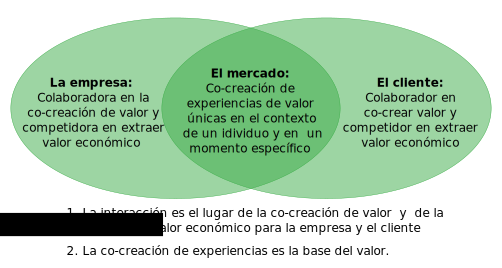
\includegraphics[width=140mm]{capitulos/graficos/esferasPrahalad} 
	\label{fig:esferasPrahalad} 

	\footnotesize
		Fuente: Prahalad y Ramaswamy, 2004, p. 11.
\end{figure}

La empresa debe centrarse en el consumidor y ha de fomentar la participación activa durante la experiencia de co-creación de valor, incluyendo la búsqueda de información, la configuración de productos y servicios, el cumplimiento y el consumo, para que las compañías puedan alcanzar las expectativas y las experiencias que los consumidores desean. (Prahalad y Ramaswamy, 2004). Por lo tanto, el mercado debe de centrarse en la convergencia de la empresa y el consumidor que da como resultado la co-creación de valor y ambos se vuelven inseparables (ver figura \ref{fig:esferasPrahalad}). Este sistema es muy exigente, pero promete ganancias sobre la eficiencia muy importantes.

Pero hay que tener en cuenta, que la empresa y el consumidor tienen una relación de colaboración pero al mismo tiempo también son competidores a la hora de co-crear valor y de obtener un beneficio económico. El mercado como un todo, se convierte en inseparable en el proceso de creación de valor, como se muestra en la figura \ref{fig:esferasPrahalad}. Hay que tener en cuenta que en los tres sectores económicos las empresas tienen como objetivo posicionarse como primera referencia en la mente del cliente cuando éste se encuentra ante la necesidad de decidirse por un producto o servicio. Las compañías que ya han conseguido ese privilegio, siguen un modelo en el que la aproximación entre lo que espera el cliente y lo que ofrece la organización, es cada vez mayor. Este enfoque pone especial énfasis en los cambios que se producen en la definición de mercado.


En resumen, Prahalad y Ramaswamy defienden que la experiencia personalizada es la base de la co-creación de valor. Pero también afirma que la integración de recursos y la interacción son necesarias en este proceso. Prahalad y Ramaswamy (2004) también defienden que el valor está incrustado en la personalidad de los individuos y no puede ser previsible por las empresas, por ello la co-creación de valor cuestiona la distinción tradicional entre la oferta y la demanda. Para que una compañía pueda ofrecer experiencias de co-creación de valor a los clientes, se ha de crear un compromiso a través de las relaciones más profundas entre ambos. Además, sostienen que el mercado debe funcionar como un foro de experiencias personalizadas donde la empresa y el cliente actúan por separado y tienen unos roles determinados. 

\subsection{Conclusiones de las teorías asociadas a la co-creación de valor}

A continuación, se va a proponer una definición propia de la co-creación de valor teniendo en cuenta que dicha co-creación de valor surge a partir de las acciones conjuntas llevadas a cabo por el cliente y por la empresa donde se supone que el individuo ha de integrar sus propios recursos y fusionarlos con los propuestos por la empresa (Vargo y Lusch, 2004). Además, ya no existen dos roles (empresa y consumidor) si no que se fusiona en uno denominado “prosumidor” (Vargo, Maglio y Akaka, 2008) ya que la empresa y el consumidor por si solos no crean valor. 

Por lo tanto, la co-creación de valor es \emph{La co-creación de valor es la interacción entre el cliente y la empresa (Grönroos, 2012) en diferentes momentos como el diseño, la producción y el consumo o disfrute del bien o servicio (Seth, Sisodia Y Sharma, 2000) integrando los recursos de ambos (Vargo y Lusch, 2004) y creando de este modo un entorno experiencial en el que los clientes puedan tener un diálogo activo para poder construir así sus propias experiencias y percepciones personalizadas (Prahalad y Ramaswamy, 2004).}

Y por último y para finalizar con el desarrollo de las principales teorías de co-creación de valor, se va a presentar el cuadro \ref{tab:comparativaTeorias} que resume las diferencias básicas entre las teorías anteriormente expuestas que son: la lógica dominante del producto, la lógica dominante del servicio, la lógica del servicio, la servucción y la co-creación de experiencias.

%\newgeometry{left=1cm}
\begin{landscape}
\begin{table}[h]
    \caption {Comparativa de las teorías asociadas a la co-creación de valor.}
	\label{tab:comparativaTeorias}
	\setlength\extrarowheight{5pt}
	
	\begin{tabular}{p{1.8cm} p{3.8cm} p{3.8cm} p{3.8cm} p{3.8cm} p{3.8cm} }
	\toprule
		                 & LDP                                                                      & LDS                                       & LS                                       & Servucción                                                                                    & Experiencias                                                          \\ \midrule
	El valor             & Valor en el intercambio.                                                 & Valor en el contexto.                     & Valor en uso a partir de la interacción. & La co-creación de valor se realiza entre la empresa y el cliente.                             & Valor en la experiencia.                                              \\
	El cliente           & Usa y destruye el valor que ha creado la empresa a través del consumo. & Co-creador de valor.                      & Creador y co-creador de valor.           & Es productor y consumidor.                                                                    & Creador de valor a través de co-creación de experiencias.             \\
	El rol de la empresa & Produce y distribuye valor.                                              & Realiza proposiciones de valor.           & Facilitadora o realizadora de valor.     & Cuida el soporte físico, los recursos humanos y la administración y organización.             & Facilitadora de entornos de experiencias o de plataformas engagement. \\
	El servicio          & Practicamente inexistente                                                & Da solución o aplicación de competencias. & Es la actividad.                         & Sin cliente no existe el servicio.                                                            & Experiencias personalizadas.                                          \\
	Los recursos         & Unidades de output y recursos operandos.                                 & Operantes y operandos.                    & Recursos y procesos de apoyo.            & Ventajas competitivas enfocadas hacia la oferta total, hacia el soporte de la oferta o ambas. & DART: diálogo, acceso, riesgo y beneficio y transparencia.            \\ \bottomrule
	\end{tabular}

	\center
	\footnotesize
	Fuente: Adaptado de Blasco, 2014. p. 61.
\end{table}
\end{landscape}



\part{Parte empírica}
\chapter{Estudio estadístico}
\label{section:parteEmpirica}
\section{Metodologías}

Una vez desarrollado el tema desde un punto de vista teórico, los pasos seguidos para realizar la parte práctica han sido los siguientes (Hernández, Fernández y Baptista, 2003):

\begin{enumerate} 
	\item Seleccionar el ambiente o lugar de estudio. Se ha elegido el sector hotelero y, en concreto, un hotel de la ciudad de Viena, Austria. 
	\item Elección de participantes o sujetos del estudio. La elección de los participantes ha sido aleatoria aunque tenían que cumplir el requisito de ser mayores de 18 años. 
	\item Inspección del ambiente o lugar de estudio. Las encuestas se realizaron en la recepción del hotel. 
	\item Trabajo de campo. Lectura y comprensión de los diferentes estadísticos para poder delimitar parámetros y estadísticos a aplicar. 
	\item Seleccionar el diseño de la investigación. Tras haber hecho la revisión de la literatura y  la obtención de los datos, se comenzó a aplicar los estadísticos elegidos y se obtuvieron los resultados. 

\end{enumerate}

Por lo tanto, el presente capítulo contiene las hipótesis del estudio de co-creación de valor, las variables seleccionadas para cada factor y los resultados del estudio estadístico. También, se discuten el diseño de investigación, la instrumentación y los métodos de análisis de datos.

\section{Características del cuestionario}

En este apartado, se describen las características del cuestionario utilizado. En el anexo \ref{anexo:7} se detalla el cuestionario y las instrucciones para llevarlo a cabo. Con dicho cuestionario se tratará de analizar la capacidad de co-creación de valor del hotel con respecto a la satisfacción, el bienestar, la participación, la fidelización de los clientes y los problemas que pueden darse a lo largo de la estancia. 

El cuestionario elegido, es de tipo mixto. Por un lado, hay preguntas dicotómicas en donde los individuos deben elegir entre las respuestas si y no. Y por otro lado, preguntas que son de tipo Likert, en las que se dan 5 opciones de respuesta al encuestado. Es una forma sencilla de calibrar opiniones específicas y da pie a crear escalas que pueden medir actitudes y valores más amplios. La escala va de uno 1 (muy insatisfecho) a 5 (muy satisfecho) con las afirmaciones propuestas (ver figura \ref{fig:escala}). Ambos grupos de preguntas serán tratados por separado y se elegirán diferentes métodos de evaluación para cada uno de ellos.

\begin{figure}[!h]
	\caption{Escala Likert aplicada en el cuestionario}
	\centering \includegraphics[width=150mm]{capitulos/graficos/escala} 
	\label{fig:escala} 
	
		\footnotesize
		Fuente: elaboración propia
\end{figure}

El huésped debe responder la opción que mejor se adapte a su realidad y con total sinceridad. Además, en cada pregunta, se da la posibilidad de aportar información extra referente a dicha cuestión. Con ello se pretende conocer más en profundidad las opiniones de los clientes, bien sean positivas o negativas para poder llevar a cabo mejoras estratégicas enfocadas al huésped.

\section{Características de la muestra}

Las 36 preguntas de la encuesta están dirigidas a huéspedes mayores de 18 años, que se han hospedado en el hotel más de una noche. El hotel está situado en capital de Austria, Viena. Hay que tener en cuenta que puede haber factores externos que alteren las respuestas de los clientes en el momento en el que se realiza el cuestionario (ver cuadro \ref{tab:respuestas}). Para controlar el efecto de estos factores, se ha realizado el test a clientes individuales en un lugar discreto y acogedor de la recepción, persiguiendo la máxima fiabilidad de los cuestionarios y solventando los problemas que pudieron surgir durante el test.

\begin{table}[h]
    \caption {Los factores que pueden afectar a las respuestas de los huéspedes}
	\label{tab:respuestas}
	\setlength\extrarowheight{5pt}
	
	\begin{tabular}{p{7cm} p{7.5cm}}
	\toprule
	Factores que pueden introducir cambios en los huéspedes                                           & Factores que pueden introducir cambios en las condiciones de administración                                                                             \\ 
\midrule
	Maduración.                 & La administradora del test.                           \\
	Aprendizaje e influencia general debida al medio social.       & El lugar elegido del hotel y su ambiente.                 \\
	Actividades anteriores a la administración del test.             & La hora y el día de la semana. \\
	Estado de salud de los huéspedes. & Sucesos no previstos durante la administración del test.                         \\ 
	\bottomrule
	\end{tabular}

	\center
	\footnotesize
	Fuente: elaboración propia
\end{table}


Se realizaron un total de 100 cuestionarios que fueron recogidos durante un período cinco meses entre diciembre del año 2014 y mayo de 2015. La figura \ref{fig:nacionalidades} muestra el porcentaje de nacionalidades que participaron en la encuesta. Además, la información demográfica general es la siguiente: de los 100 encuestados, el 45\% (45) eran hombres y el 55\% (55) eran mujeres. A efectos descriptivos, se considera una muestra lo suficientemente grande cuando $ n>30 $ por lo tanto, se ha considerado que la muestra es suficiente para llevar a cabo el estudio estadístico a un nivel de seguridad del 95\% (Jimenez, 1983).

\begin{figure}[!h]
	\caption{Nacionalidades de los encuestados}
	\centering 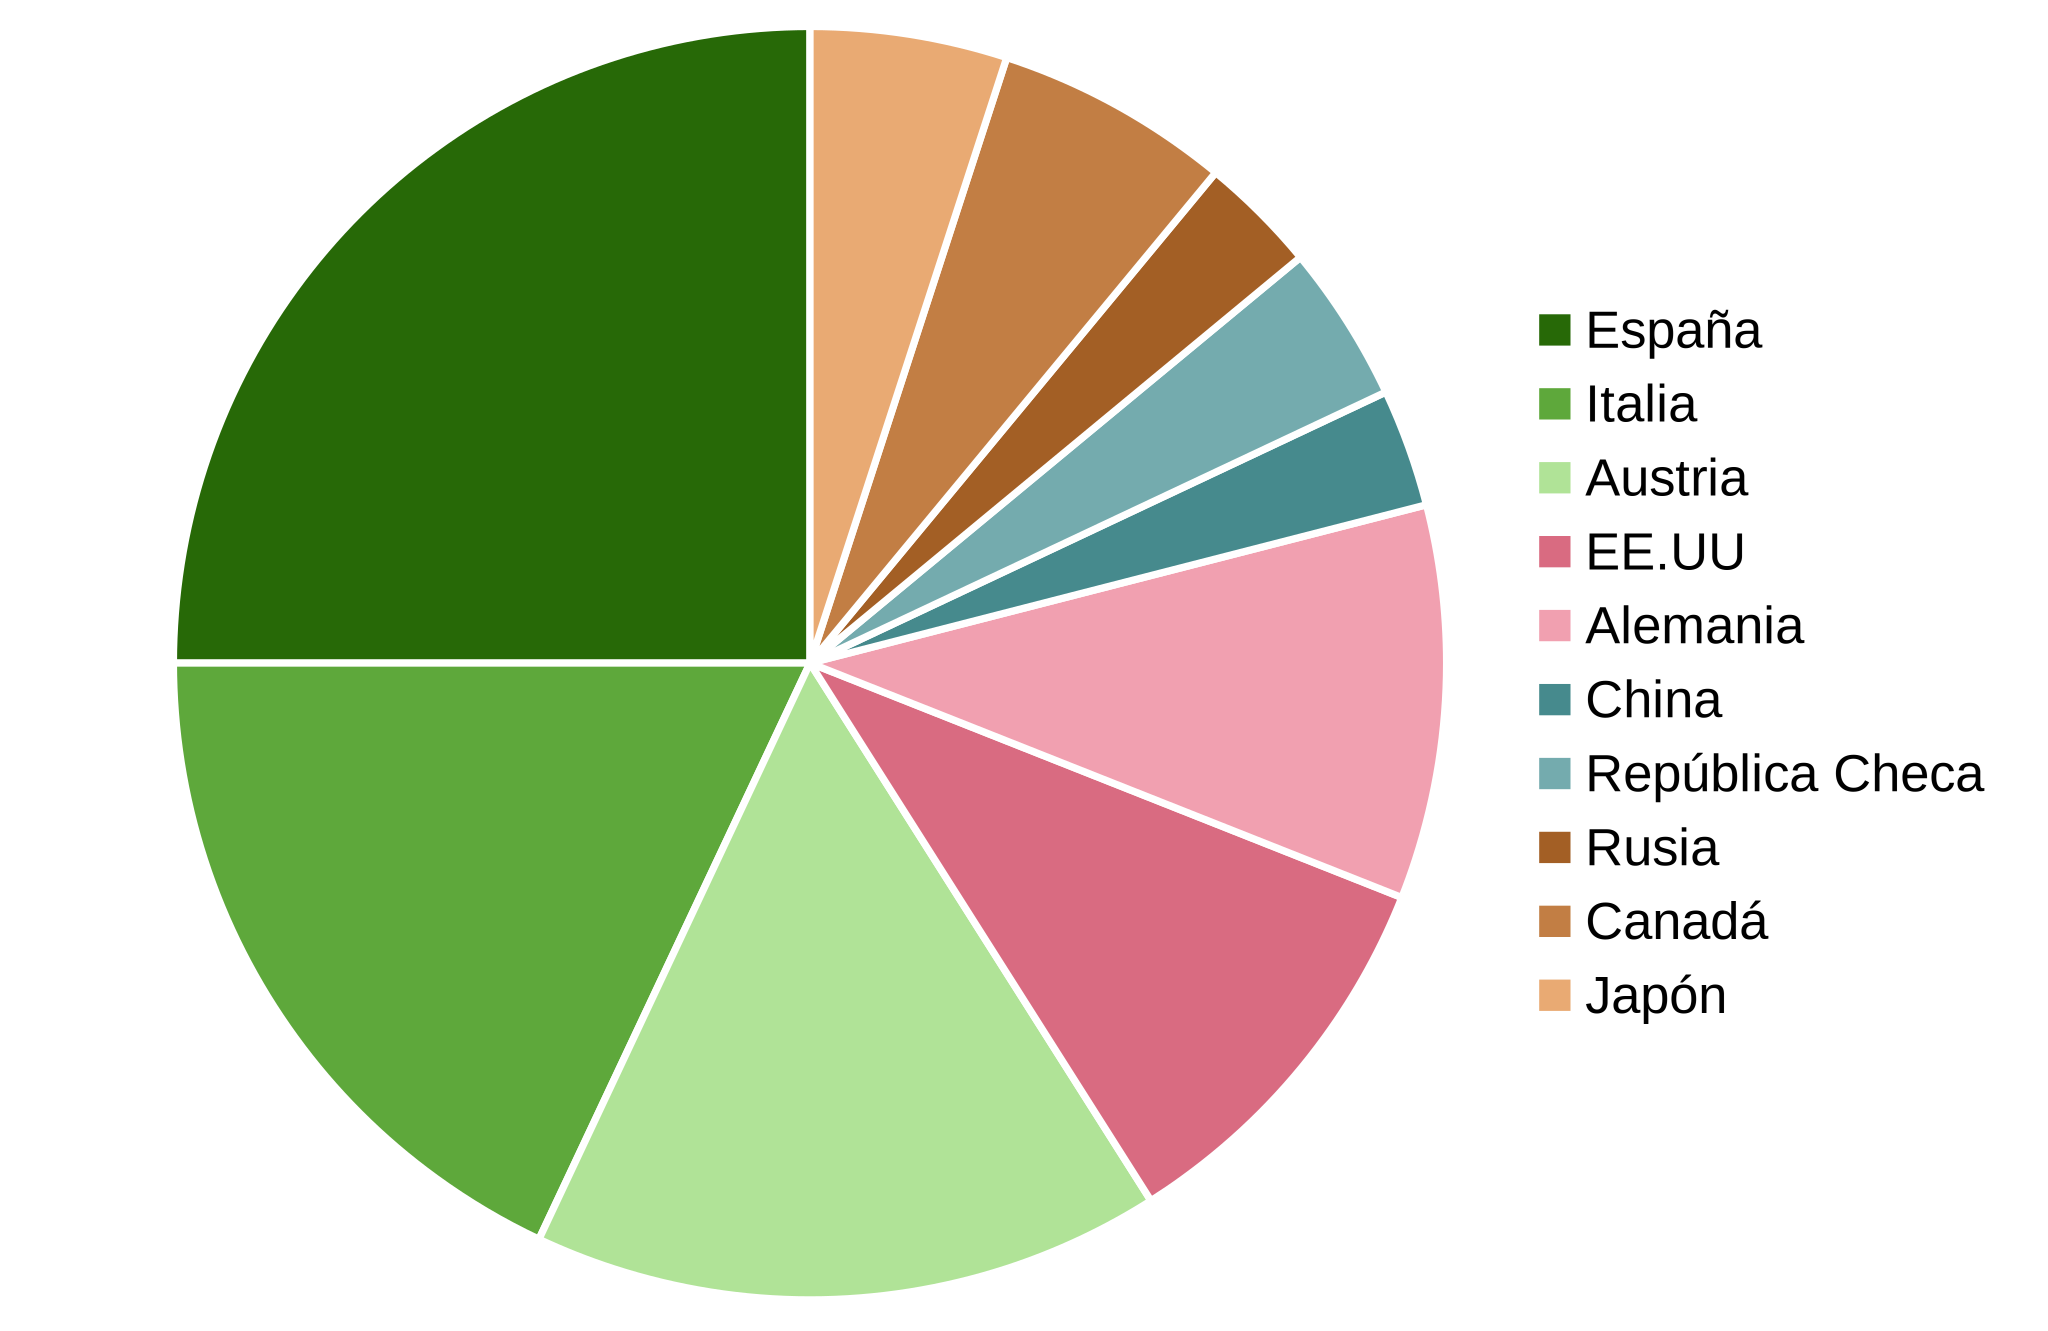
\includegraphics[width=120mm]{capitulos/graficos/nacionalidades} 
	\label{fig:nacionalidades} 
	
		\footnotesize
		Fuente: elaboración propia
\end{figure}

\section{Definición de los factores}

Para poder llevar a cabo este estudio, es necesario definir los factores que se quieren analizar y explicar el porqué de su elección. Los factores elegidos son apoyados por diversos autores que recoge Frances (2013), autora que se va a tener en cuenta en este presente epígrafe.

\subsection{Co-creación}

Frances (2013) indica que algunos investigadores (Cova et al., 2011, y Arvidsson, 2008) creen que fundamental la voluntad del cliente a la hora de trabajar y de participar con la empresa. Sin esta interacción la co-creación de valor no es posible. Sin embargo, si la empresa propone un proceso de co-creación de valor con el cliente, hay que tener en cuenta que los consumidores han de tomar la decisión de si desean o no co-crear valor con el hotel. Para Frances (2013), la co-creación se basa en la unión de dos partes, en este caso serían el huésped y el hotel. Por lo tanto, en este estudio se pretende medir cómo afecta la disposición de los huéspedes a la hora de co-crear valor trabajando codo con codo con el hotel, compartiendo sus ideas, problemas y sentimientos de bienestar, expresando sus opiniones bien sean satisfactorias o insatisfactorias, midiendo el grado de fidelización y de participación de los clientes. Para ello, el hotel ha de contar con un personal adecuado que sepa transmitir los valores de la cadena hotelera, también ha de estar abierto a escuchar e incorporar las ideas de cada huésped, y además ha de ser capaz de facilitar la co-creación y proporcionar un ambiente que propicie la unión de ambas partes para que los clientes sientan que sus opiniones son escuchadas y valoradas, y fomentar que el cliente se sienta valorado y mimado por el hotel. Esta continua transformación es vital para que surja la co-creación de valor (Frances, 2013). 

\subsection{Satisfacción}

Según Frances (2013), la satisfacción puede confundirse con el bienestar del cliente. Si la satisfacción aumenta, el bienestar también debería de hacerlo. Pero en el presente trabajo se va a considerar como satisfacción el momento en el que el cliente evalúe la relación de experiencias que ha establecido con el hotel teniendo en cuenta también su nivel de vida. Por lo tanto, este factor indicará que si el cliente está lo suficientemente satisfecho con lo que el hotel le ha proporcionado a lo largo de su estancia, entonces aumentará la posibilidad de que el consumidor vuelva. También, se podrá evaluar si el cliente cree que está acorde lo que se le ha ofrecido con lo que ha pagado por ello. Además, podrá utilizar el boca a boca para expresar su satisfacción a a través de las redes sociales o personalmente acerca del hotel.

\subsection{Bienestar}

Este factor tiene en cuenta aspectos como la valoración del medio ambiente que rodea al hotel y el trato percibido por el cliente por parte del personal (Frances, 2013). Según Frances (2013), los efectos económicos como los ingresos, el empleo, el coste de vida, los precios de bienes y servicios, y los impuestos, afecta al bienestar percibido por un huésped. Se puede dar el caso de que algunos clientes puedan sentirse limitados a participar en estos procesos de co-creación porque éste no disponga de los recursos personales necesarios para contribuir al intercambio de experiencias, y por lo tanto se ve afectado su bienestar. Por otro lado, los efectos ambientales tales como la contaminación o el tráfico, también pueden influir en el bienestar del huésped. No se trata de una variable fundamental dentro del proceso de co-creación de valor, pero si que hay que tener en cuenta que si un cliente busca tranquilidad y se le ofrece una habitación con orientación a una calle muy transitada y con tráfico pesado o con zonas contaminadas, esto daría lugar a una negativa experiencia de alojamiento y un nivel de bienestar muy bajo. Este efecto podría provocar que el cliente no vuelva al hotel y viceversa en caso contrario. Por lo tanto, con el fin de mejorar el bienestar del cliente, las interacciones entre el personal del hotel y los huéspedes en los procesos de co-creación han de ser positivas.

\subsection{Participación}

Según indica Frances (2013), los autores Grissemann y Stokurger-Sauer (2012) y Lee (2012) demostraron que en la co-creación de valor influye el grado de participación que el cliente tiene. En el presente estudio, se va a medir a través de las implicaciones que los clientes tienen con otros huéspedes; analizando si participan activamente en ONGs cercanas al hotel; o teniendo en cuenta si los huéspedes administran los recursos naturales de forma responsable; analizando si contribuye al desarrollo económico tanto de la ciudad de Viena como de este hotel en concreto y por último, si está dispuesto a publicar su opinión en Tripadvisor que es la Web líder mundial de opiniones de hoteles.

\subsection{Problemas}

En el presente trabajo se quiere evaluar si los problemas afectan a los procesos de co-creación y para ello se va tener en cuenta si a los huéspedes les surgen un gran número de problemas y al mismo tiempo si estos problemas los reportan al personal del hotel y este a su vez los resuelve eficazmente. Se va a suponer que si existe gran cantidad de problemas, los procesos de co-creación no se desarrollarán favorablemente y viceversa.

\subsection{Fidelización}

Se trata de efectos sociales, donde se tiene en cuenta la calidad de las interacciones entre los clientes y los empleados y las posteriores relaciones resultantes. Se espera que los efectos sociales de esta fidelización estén directamente relacionados con la co-creación. Para ello, se requiere mucha interacción duradera en el tiempo entre el huésped y el hotel para crear una relación de fidelización. Esto se puede conseguir si un cliente es capaz de trabajar de manera efectiva junto con la empresa hotelera, propiciando un desarrollo de la relación mucho más fuerte y que tiene un efecto positivo en la fidelización del cliente con la cadena hotelera. En cambio, si la relación no tiene éxito y el huésped siente que el hotel no le proporciona lo que desea, o siente que no tiene la oportunidad de participar en el proceso de co-creación de valor, entonces la relación de fidelización no surgirá (Frances, 2013).

\section{Formulación de las hipótesis}

Una vez descritos los factores que se quieren estudiar, se ha de recordar que principal objetivo del estudio es el de medir el grado de relación entre la co-creación de valor por parte de los clientes y la satisfacción y el bienestar, además, se quiere determinar la relación sobre la implicación que los clientes asumen en el programa de fidelización, la participación y cómo afectan los problemas que les surgen a los huéspedes con respecto a la co-creación de valor con el hotel. Por ello, se van a plantear las siguientes  hipótesis (ver figura \ref{fig:hipotesis}):

\begin{itemize}
\item H1: Existe una relación directa entre la co-creación de valor y la satisfacción del cliente en el hotel.

\item H2: Existe una relación directa entre la co-creación de valor y el bienestar del cliente en el hotel.

\item H3: Existe una relación directa entre la co-creación de valor y la participación del cliente con el hotel.

\item H4: Existe una relación directa entre la co-creación de valor y los problemas que le surgen a los huéspedes en el hotel.

\item H5: Existe una relación directa entre la co-creación de valor y la fidelización de los clientes.
\end{itemize}

\begin{figure}[!h]
	\caption{Hipótesis}
	\centering 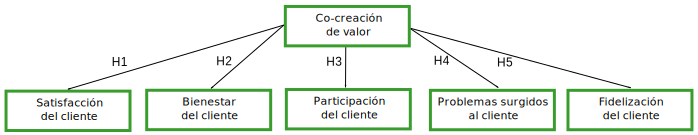
\includegraphics[width=150mm]{capitulos/graficos/hipotesis} 
	\label{fig:hipotesis} 
	
		\footnotesize
		Fuente: elaboración propia
\end{figure}

Estas hipótesis se pueden relacionar con las teorías sobre la co-creación de valor desarrolladas en el capítulo \ref{section:cocreacion} del presente trabajo. En primer lugar, la integración de recursos que recoge la lógica dominante del servicio se puede relacionar con la hipótesis H3 que evalúa si hay una relación directa entre la co-creación de valor y la participación del huésped. Lo hace a través de cuestiones por las que se integran recursos en el proceso co-creativo, por ejemplo, con la participación en ONGs, la administración de los recursos naturales, el desarrollo económico por parte del huésped, etc. En segundo lugar, se encuentra la interacción que rompe con los procesos de producción de productos para desarrollar uno propio para los servicios. Eigler y Langeard desarrollan la teoría de la servucción y la escuela nórdica de Grönroos la lógica del servicio. Las hipótesis H4 y H5, se corresponde con el análisis de la relación directa entre la co-creación de valor y los problemas que le surgen al cliente y la fidelización de éste respectivamente. Son los factores que requieren que el personal del hotel y el huésped interactúen entre sí. Y por último, las hipótesis H1 y H2, evalúan la relación que tiene la co-creación de valor con la satisfacción y con el bienestar, encajan con la teoría de Prahalad y Ramaswamy que defienden las relaciones personalizadas entre la empresa y el cliente para que éste último pueda interaccionar con el entorno empresarial y cree experiencias personales de co-creación de valor tanto para la empresa como para sí mismo. 

\section{Análisis de datos}

En esta sección del capítulo 2, se resumirán los pasos a seguir en el análisis de datos. Tras el proceso de recogida de datos, éstos se han procesado y ordenado con el fin de llevar acabo un análisis fiable. Para ello, se ha elegido el programa informático IBM SPSS Statistics 23. Se trata del Software estadístico líder mundial utilizado para resolver problemas empresariales y de investigación por medio de análisis ad-hoc, pruebas de hipótesis y análisis predictivo (ibm.com, 2015).

Como el cuestionario es de tipo mixto, se van a realizar dos estudios preliminares diferentes para determinar qué variables se asocian a los diferentes factores a estudiar. Ambos análisis, se van a dividir en dos estudios a su vez. En el primero de ellos, se va a realizar un análisis factorial y posteriormente un contraste de hipótesis a través de la varianza denominado ANOVA. Para el estudio de las variables dicotómicas el análisis factorial es subjetivo y el investigador decidirá las variables que han de incorporarse a cada factor (Montoya, 2007; Mora, 2010), ya que el cuestionario dicotómico fue elaborado con esta intención. En el cuadro \ref{tab:criterios}, se pueden apreciar los cálculos que se van a llevar a cabo a lo largo del análisis y los límites que propone la literatura.

\begin{table}[h]
    \caption {Criterios utilizados en el estudio estadístico}
	\label{tab:criterios}
	\setlength\extrarowheight{5pt}
	
	\begin{tabular}{p{2.1cm} p{3.5cm} p{4.2cm} p{4.1cm}}
	\toprule
	Análisis factorial	& Cargas factoriales	& $ > 0,4 $	& Everitt y Hothorn, (2011)	\\
						& Autovalores			& $ > 1 $		& Everitt y Hothorn, (2011)	\\
						& Alfa de Cronbach		& $ > 0,7 $	& Everitt y Hothorn, (2011)	\\
						& Varianza acumulada	& $ > 0,65 $	& Everitt y Hothorn, (2011)	\\
						& Test de esfericidad de Bartlett & $ p < 0.05 $ & Blasco, 2014; Mora, 2012; Thorndike, 1989; Montoya, 2007	\\
						& Kaiser Meyer Olkin	& \pbox{4.2cm}{
						$ KMO < 0,5 $: no existe correlación. \\
						$ 0,5 < KMO < 0,6 $: nivel de correlación medio. \\
						$ KMO > 0,7 $: alta correlación. \\
						} & Blasco, 2014; Mora, 2012; Thorndike, 1989; Montoya, 2007	\\
	\midrule
	Contraste de hipótesis	& ANOVA				& $ p < 0.05 $	& Rolan, 2014 \\
	\bottomrule
	\end{tabular}
	
	\center
	\footnotesize
	Fuente: elaboración propia
\end{table}


\subsection{Estudio 1}

\subsubsection{Análisis factorial}

El análisis factorial tuvo sus orígenes a comienzos del siglo XX y es conocido como una técnica estadística de interdependencia que se caracteriza por su versatilidad. Esta técnica consiste en analizar un grupo de variables que se analizan al mismo tiempo y en conjunto (Menendez y Rondón, 2012). Uno de los objetivos de este análisis es tratar de definir grupos de variables que a partir de ahora se les va a denominar factores, y que deben de estar altamente correlacionados entre sí. Otros dos objetivos son la reducción de la complejidad en cuanto al número de variables a utilizar en el estudio y eliminar variables redundantes o que aporten poca información. Por lo tanto, va a permitir explicar el fenómeno de la co-creación de valor deforma más minuciosa. Y por último, va a ayudar a identificar problemas de multicolinealidad evaluando si las variables altamente correlacionadas pueden afectar a la construcción de los modelos de regresión o de análisis multivariantes (Montoya, 2007).

Los cálculos se van a realizar en SPSS a partir de la \emph{matriz original de datos} \footnote{Se corresponde a la matriz que contiene las 36 variables bajo estudio con las correspondientes 100 observaciones por variable.} creada en un documento Excel. En el anexo \ref{anexo:8} se pueden encontrar todos los resultados de este análisis. En primer lugar, SPSS calculará la \emph{matriz de correlaciones} de las variables medidas en escala Likert, que mide y muestra la interdependencia entre cada pareja de variables y todas al mismo tiempo (Peña, 2002; Lemos, Vallejo y Sandoval, 2002; Montoya, 2007). Al mismo tiempo, calculará el determinante de esta matriz de correlaciones cuyo valor ha sido $ D = 4,85E-009 $, el cual se considera muy bueno porque significa que hay variables que poseen intecorrelaciones muy altas y se puede continuar con el análisis (Lemos, Vallejo y Sandoval, 2002; Montoya, 2007).

Por otro lado, se calcula el índice de \emph{Kaiser Meyer Olkin} (KMO) cuyo valor ha sido de 0,611 que indica que existe un nivel de correlación medio una vez que se han descontado los efectos lineales de otras variables (Blasco, 2014; Mora, 2012; Thorndike, 1989: Montoya, 2007). Además, la \emph{prueba de esfericidad de Bartlett} ha resultado tener una fiabilidad de $ p = 0,000 $, por lo tanto, el nivel de significación es menor a p < 0.05, lo que significa que se rechaza la hipótesis nula y se continúa con el análisis factorial (Blasco, 2014; Mora, 2012; Jackson, 1993; Bossé et. al. 1999; Montoya, 2007).

En tercer lugar, se calcula la \emph{matriz anti-imagen} donde se ha observado que no existen a penas coeficientes cero y por lo tanto se continua el análisis (Montoya, 2007).

El siguiente paso es comprobar la \emph{varianza total explicada} que es la que agrupa a las variables a partir del total de la variabilidad del número de variables. El límite que establece la comunidad para aceptar la fiabilidad del estudio y continuarlo, es que la varianza acumulada debe de ser mayor a 65\% y en el caso a estudiar, dicha varianza adquiere un valor de 66,533848\% (Damey, Andams y Freites, 1992).

La función del \emph{gráfico de sedimentación} es localizar visualmente un codo o punto de inflexión,que puede ser definido como el punto donde los valores propios forman una tendencia lineal descendente (Reise, Waller y Comrey, 2000).

A continuación, se obtendrá la \emph{matriz de componentes} con la extracción inicial y una segunda matriz con la peculiaridad de que es la matriz de componentes rotada por VARIMAX. Esta rotación, se realiza con la finalidad de lograr una solución que facilite la interpretación (Montoya, 2007). La rotación Varimax es uno de los métodos más utilizados en la actualidad para la formación de los componentes cuyos ítems serán aceptados si superan la barrera del 0,4 (Martínez, 2008; Montoya, 2007). Las variables finales asignadas a cada factor son las mostradas en el cuadro \ref{tab:variablesFactores1}. Y se corresponde con la solución que ha proporcionado SPSS a través del cuadro de resultados denominada \emph{matriz de factores rotados}, donde los coeficientes de esta matriz indican cuánto explica cada variable los factores surgidos y por lo tanto los encasilla en un factor u otro teniendo en cuenta dos aspectos: 1) el coeficiente ha de ser mayor a 0,40 y, 2) el factor elegido ha de ser superior en 0,10 al segundo mejor factor (universidad de Monterrey, 2012). La denominación de los factores encontrados, McDaniel et al. (1999) señalan que es algo subjetivo y se requiere de una combinación de intuición y conocimiento por parte del investigador sobre las variables.

\begin{table}[h]
    \caption {Variables de los factores del estudio 1}
	\label{tab:variablesFactores1}
	\setlength\extrarowheight{5pt}
	
	\begin{tabular}{p{11.8cm} p{2.9cm}}
	\toprule
	¿Recomendará este hotel? & \\
	¿Volverá a este hotel? & \\
	¿Está satisfecho con baño de la habitación? &  \\
	¿Está satisfecho con las amenidades del baño y los productos de aseo que el hotel el proporcionó? & Satisfacción \\
	¿Cómo evalúa la relación calidad – precio global? & \\
	¿Está satisfecho con el servicio de desayunos? & \\
	\midrule
	¿Cómo fue su experiencia global en el hotel? & \\
	¿Cómo fue su experiencia global con la habitación? & \\
	¿Qué le pareció la atmósfera del hotel (música, aroma, iluminación, decoración, mobiliario)? & \\
	¿Qué le pareció la cama? & Bienestar \\
	¿Cómo fue su experiencia durante el Check in? & \\
	¿Cómo evalúa los servicios de Internet y WiFi en el hotel? & \\
	¿Cómo evalúa la atención al huésped en general en el hotel? & \\
	¿Su reserva antes de llegar al hotel fue gestionada eficientemente? & \\
	\midrule
	¿Cómo ha sido la actitud y proactividad de los empleados durante su estancia en el hotel? & \\
	¿Cómo ha sido el trato de los empleados a lo largo del check out? & Co-creación \\
	¿Sintió que le mimamos durante su estancia? & \\
	¿Le parece adecuado el plan de fidelización que propone el hotel? & \\

	\bottomrule
	\end{tabular}
	
	\center
	\footnotesize
	Fuente: elaboración propia
\end{table}


\newpage

A continuación, en el cuadro \ref{tab:afe} se van a resumir algunos de los resultados obtenidos en el análisis factorial y por los cuales se ratifica que estos son los factores a analizar en el contraste de hipótesis.

\begin{table}[h]
    \caption {Análisis exploratorios de fiabilidad y dimensionalidad}
	\label{tab:afe}
	\setlength\extrarowheight{5pt}
	
	\begin{tabular}{p{1.9cm} p{1.9cm} p{1.9cm} p{1.9cm} p{1.9cm} p{1.9cm} p{1.7cm}}
	\toprule
	Factor	& Coeficiente menor de cargas factoriales	& Autovalores & Alfa de Cronbach & Varianza explicada & Test de esfericidad de Bartlett & KMO \\
	\midrule
	Co-creación	 & 0,7	& 2,511	& 0,783	& 28,106 & 0,000 & 0,665 \\
	Satisfacción & 0,45	& 3,465	& 0,837	& 22,524 & 0,000 & 0,812 \\
	Bienestar	 & 0,57	& 3,886	& 0,835	& 28,106 & 0,000 & 0,814 \\
	\bottomrule
	\end{tabular}
	
	\center
	\footnotesize
	Fuente: elaboración propia
\end{table}


\newpage


\subsubsection{Contraste de hipótesis}

Una vez que se han verificado los factores a través del análisis factorial, a continuación se van a testar las dos primeras hipótesis propuestas con el método ANOVA. Este método, viene de la terminología inglesa \emph{analysis of variance}, cuya traducción al castellano es análisis de la varianza.

El análisis ANOVA permite relacionar los factores satisfacción y bienestar con el factor de co-creación de valor de una forma directa. De esta forma, se podrán contrastar las hipótesis nulas planteadas al comienzo del capítulo. Los cálculos llevados a cabo con SPSS se pueden apreciar en el anexo \ref{anexo:9}.
La interpretación de los resultados relevantes mostrados en el cuadro \ref{tab:anovaSB}, determinan la relación existente entre la satisfacción y el bienestar con la co-creación de valor. En primer lugar, se va a analizar la satisfacción, donde su nivel crítico asociado al estadístico es $ F_{4,929} $ es $ p = 0,04 $. El criterio establece que $ p = 0,000 < 0,05 $, por lo tanto, este resultado indica que el modelo explica una parte significativa de la variación observada en el factor co-creación. Como consecuencia, se puede confirmar la hipótesis 1 que afirma que existe una relación directa entre la satisfacción y la co-creación de valor. En cambio para el factor bienestar, el nivel crítico asociado al estadístico $ F_{2,111} $ es $ p = 0,107 $ que es mayor que 0,05, lo que hace que se la hipótesis 2 se rechace y se establezca que no existe una relación directa entre el bienestar y la co-creación de valor.

\begin{table}[h]
    \caption {Resultados ANOVA de la satisfacción y el bienestar con respecto a la co-creación de valor}
	\label{tab:anovaSB}
	\setlength\extrarowheight{5pt}
	
	\begin{tabular}{p{4.0cm} p{4.6cm} p{3.1cm} p{2.1cm}}
	\toprule
	Origen	& Media cuadrática	& F & Sig. \\
	\midrule
	Satisfacción & 1,474	& 4,929	& 0,004 \\
	Bienestar	 & 1,199	& 2,111	& 0,107 \\
	\bottomrule
	\end{tabular}
	
	\center
	\footnotesize
	Fuente: elaboración propia
\end{table}


\subsection{Estudio 2}

\subsubsection{Análisis factorial}

En el caso de las cuestiones dicotómicas, a la hora de realizar el cuestionario se establecieron tres grupos y se ha creído conveniente que esos grupos de variables sean los factores finales para el análisis (Montoya, 2007; Mora, 2010).

Para comprobar si los factores son fiables se ha calculado el coeficiente \emph{alfa de Cronbach}, que fue propuesto por primera vez en 1951 por Lee Cronbach. Se trata de un estadístico que estima la confiabilidad de una prueba a partir de la suma de varias mediciones (Thorndike, 1989,1996; Muñiz, 1996). A través del cálculo de los alfas de Cronbach, se puede valorar la fiabilidad de las escalas de medida elegidas y evaluar si los huéspedes han contestado de forma coherente a este tipo de preguntas dicotómicas. Además, se han contrastado los resultado con el coeficiente de Kuder Richardson (KR-20), ya que es análisis que más utilizado para medir variables dicótomicas, los resultados han sido idénticos (ver anexo \ref{anexo:10}). Por lo tanto, los factores que se han delimitado para las cuestiones dicotómicas son: participación, problemas y fidelización; quedando las variables enumeradas tal y como aparecen en el cuadro \ref{tab:variablesFactores2}). 

\begin{table}[h]
    \caption {Variables de los factores del estudio 2}
	\label{tab:variablesFactores2}
	\setlength\extrarowheight{5pt}
	
	\begin{tabular}{p{11.8cm} p{2.9cm}}
	\toprule
	¿Le gustaría enviar su opinión a Tripadvisor a través de esta encuesta?	& \\
	¿Proporciona usted productos y servicios sostenibles a otros huéspedes?	& \\
	¿Promueve la oferta cultural de la ciudad de Viena?	& Participación \\
	¿Apoya las actividades de las ONGs y otras organizaciones locales?	& \\
	¿Administra los recursos naturales de una forma responsable (agua, energía, desperdicios)?	& \\
	¿Contribuye al desarrollo económico de este hotel con su estancia?	& \\
	\midrule
	¿Tuvo algún problema?	& Problemas \\
	¿Reportó ese problema?	& \\
	\midrule
	¿Es miembro del programa de fidelidad? & \\
	¿Durante su estancia, ¿le informaron sobre los beneficios del programa de fidelidad? & Fidelización \\
	¿Se hizo miembro del programa de fidelidad durante la última estancia? & \\
	\bottomrule
	\end{tabular}
	
	\center
	\footnotesize
	Fuente: elaboración propia
\end{table}


\subsubsection{Contraste de hipótesis}

Una vez se han delimitado los factores, a continuación se va a proceder a testar las tres últimas hipótesis propuestas con el método ANOVA como ya se ha realizado en el estudio 1. Al tratarse de variables categóricas, se ha utilizado otra de las opciones que propone SPSS. Se pueden comprobar los resultados obtenidos en el anexo \ref{anexo:11}.

La interpretación de los resultados relevantes mostrados en el cuadro \ref{tab:anovaPPF}, determinan la relación existente entre la participación, los problemas y la fidelización con la co-creación de valor. En primer lugar, se va a analizar la participación, donde su nivel crítico asociado al estadístico es $ F_{3,686} $ es $ p = 0,04 $. El criterio establece que $ p = 0,000 < 0,05 $, por lo tanto, este resultado indica que el modelo explica una parte significativa de la variación observada en el factor co-creación. Como consecuencia, se puede ratificar la hipótesis 3 que afirma que existe una relación directa entre la participación y la co-creación de valor. En cambio para el factor problemas, el nivel crítico asociado al estadístico $ F_{0,03} $ es $ p = 0,959 $ que es mucho mayor que 0,05, lo que hace que la hipótesis 4 se rechace y se establezca que no existe una relación directa entre el los problemas surgidos al huésped en el hotel y la co-creación de valor. Y por último, el factor fidelización tiene un nivel crítico asociado al estadístico de $ F_{3,463} $ es $ p = 0,023 $, por lo tanto, este resultado indica que el modelo explica una parte significativa de la variación observada en el factor co-creación. Como consecuencia, se puede ratificar la hipótesis 5 que afirma que existe una relación directa entre la fidelización del huésped y la co-creación de valor.

\begin{table}[h]
    \caption {Resultados ANOVA de la participación, los problemas y la fidelización con respecto a la co-creación de valor}
	\label{tab:anovaPPF}
	\setlength\extrarowheight{5pt}
	
	\begin{tabular}{p{2.9cm} p{2.9cm} p{2.9cm} p{2.9cm}}
	\toprule
	Origen	& Media cuadrática	& F & Sig. \\
	\midrule
	Participación	& 17,174	& 3,686	& 0,04 \\
	Problemas	 	& 0,03		& 0,03	& 0,959 \\
	Fidelización	& 9,069		& 3,463	& 0,023 \\
	\bottomrule
	\end{tabular}
	
	\center
	\footnotesize
	Fuente: elaboración propia
\end{table}


A continuación, se va a presentar el cuadro \ref{tab:hipotesis} en el que se puede apreciar la solución final de la parte empírica de este trabajo y por lo tanto la solución final al objetivo principal de este proyecto que es determinar las relaciones de diferentes factores con la co-creación de valor. Además, se va a proceder a realizar una comparativa entre los resultados obtenidos y la visión que el hotel tiene acerca de estas relaciones gracias a la entrevista realizada a un directivo del hotel. En el anexo \ref{anexo:12} se puede encontrar las preguntas realizadas en la entrevista.

\begin{table}[h]
    \caption {Solución del contraste de hipótesis}
	\label{tab:hipotesis}
	\setlength\extrarowheight{5pt}
	
	\begin{tabular}{p{2.1cm} p{9.7cm} p{2.3cm}}
	\toprule
	Número	& Hipótesis	& Se acepta / se rechaza \\
	\midrule
	H1 & Existe una relación directa entre la co-creación de valor y la satisfacción del huésped en el hotel.	& Aceptada \\
	H2 & Existe una relación directa entre la co-creación de valor y el bienestar del huésped en el hotel.	& Rechazada \\
	H3 & Existe una relación directa entre la co-creación de valor y la participación del huésped con el hotel.	& Aceptada \\
	H4 & Existe una relación directa entre la co-creación de valor y los problemas que le surgen a los huéspedes en el hotel.	& Rechazada \\
	H5 & Existe una relación directa entre la co-creación de valor y la fidelización de los huéspedes.	& Aceptada \\	
	\bottomrule
	\end{tabular}
	
	\center
	\footnotesize
	Fuente: elaboración propia
\end{table}


Tal como se puede apreciar en el cuadro \ref{tab:hipotesis}, el bienestar, la participación y la fidelización de los huéspedes tienen una relación directa con la co-creación de valor; y por el contrario, el bienestar y el surgimiento de problemas en el hotel no tienen una relación directa con la co-creación de valor. En el anexo \ref{anexo:13}, se explica la relación entre el hotel y los clientes, desde el punto de vista del director de hotel. A continuación, teniendo en cuenta estas explicaciones, se va a dar sentido a los resultados de las hipótesis formuladas en el presente capítulo teniendo en cuenta el punto de vista del director del hotel.

Según el estudio realizado, existe una relación directa entre la co-creación de valor y la satisfacción del huésped. Señala la importancia de la variable relación calidad – precio en la percepción de satisfacción del cliente. Además, para el director del hotel, que un cliente se vaya satisfecho garantiza dos cosas: que volverá y que hablará del hotel a sus familiares y amigos, produciendose así la mejor y la más económica de todas las publicidades de las que disponen en la cadena. Además, afirma que cuando se da este caso, la reputación del establecimiento aumenta considerablemente y como consecuencia se generan ingresos. Como bien se ha tratado a lo largo del trabajo, no todos los clientes son iguales, y el director del hotel lo ratifica. Existen multitud de perfiles de clientes, tantos como motivos de viajes, nacionalidades, etc. Pero también destaca que no siempre tienen razón y no siempre se les puede hacer caso en todo lo que proponen. Por ejemplo, realizar una reforma en el bar para convertirlo en estilo chill out se puede considerar como una muy buena idea y que revalorizaría al hotel, pero otro cliente puede opinar lo contrario. Además, hay que tener en cuenta que el hotel puede no disponer de los medios y de la financiación para llevarlo a cabo. También le surge la preocupación del boca a boca, ya que si los clientes han finalizado la estancia con un grado alto de insatisfacción harán uso de Internet y de las redes sociales para divulgar su frustración. Por lo tanto, se puede decir que si el cliente finaliza satisfecho, tanto el hotel como el huésped habrán conseguido co-crear valor conjuntamente.

En segundo lugar, el estudio establece que no existe una relación directa entre la co-creación de valor y el bienestar del huésped. Esta cuestión entra en discordancia con la visión que el director tiene sobre este punto. Éste, asume que si el cliente no ha obtenido el bienestar esperado se debe a que el hotel no ha sabido adaptarse a las necesidades del huésped. El objetivo que tiene el hotel con respecto a este factor, es dar cabida a las expectativas del cliente y superarlas en todo momento. Para hacer que el huésped desarrolle su bienestar, en cada hotel existe una persona que ostenta el cargo de “Guest experience”, o traducido al castellano “jefe de calidad”. Esta persona es la encargada de atender a los clientes y de hacerles más agradable su estancia, pero también es la responsable de inculcar los valores de la cadena a los trabajadores.

El primer paso en la formación del personal del hotel, es una reunión donde se les facilita un manual de conducta y otros aspectos a tratar. Por ejemplo, la fraseología que los empleados han de utilizar con el cliente. Hay departamentos que al tener más contacto con el cliente, se ha de prestar especial énfasis en esta parte. Además, en dicha reunión se emplean vídeos desarrollados por el departamento de recursos humanos para poner ejemplos de cómo se ha de actuar en un determinado momento y circunstancia. También, hay que tener en cuenta que a mayor responsabilidad en el cargo que se ostente dentro de la empresa, mayor conocimiento se exige sobre el cliente. Por ello, este aspecto es muy importante para el hotel, y se puede decir que se discrepa con los resultados obtenidos en el estudio.

En cuanto a la relación directa existente, según los resultados del estudio, entre la co-creación de valor y la participación del cliente, el director del hotel destaca la importancia de que el cliente se involucre de una forma muy activa, bien sea por iniciativa propia o del hotel. Esta participación genera reputación y riqueza, y la generación de riqueza es fundamental para la empresa. Sin dinero y sin retorno del cliente, no hay beneficio y si no hay beneficio el negocio no es rentable. Además, la participación del huésped también puede generar publicidad a través del boca a boca a parte de riqueza. Por lo tanto, queda demostrado que la co-creación de valor y la participación del cliente con el hotel van de la mano.

Por otro lado, el estudio indica que no existe una relación directa entre la co-creación de valor y los problemas que le puede surgir al huésped, se trata de un resultado totalmente acorde con lo esperado y con lo que el director del hotel ha expresado. La forma de interactuar en el momento en el que surgen problemas es mediante la comunicación directa entre cliente y personal del hotel. Otro modo, es mediante las encuestas de calidad donde queda registrada la opinión del cliente, y es en ese momento en el que la cadena hotelera acepta que existe un problema y puede o no otorgar los medios físicos o monetarios para poder atajar los problemas. Pero la realidad, según indica el director con total sinceridad, es que muchos de los problemas se almacenan y no se solventan en un largo periodo de tiempo, ya que siempre suelen existir otras prioridades.

Y por último, la relación directa que hay entre la co-creación de valor y la fidelización del huésped es un punto muy destacado por el director del hotel. Este programa de fidelización que propone la cadena hotelera es idéntico en cada hotel independientemente de su localización. Esto supone, que el cliente va a recibir el mismo trato y las mismas ventajas en un hotel de una ciudad u otra. Para que esta fidelización se produzca, la compañía tiene que proporcionar al cliente unas ventajas y un trato superior a los competidores. Una vez que un cliente que pertenece al plan de fidelización y abandona un hotel, la cadena se pone en contacto con él para que éste pueda valorar su estancia. Todas las sugerencias se archivan para una futura ocasión aunque el servicio post venta como tal no exista. Para solventar este problema, la cadena está desarrollando una nueva base de datos con la que pretenden personalizar las experiencias de los huéspedes fidelizados facilitándoles y sugiriéndoles opciones de viaje adecuadas a sus gustos. El mayor fracaso que puede sufrir el hotel es no cumplir las expectativas de un cliente por un motivo u otro. Por ello, que se de una relación de fidelización, hace que la co-creación de valor surja de una forma espontánea. 

Se puede concluir el presente estudio, afirmando que son resultados esperados a excepción del bienestar, ya que podría darse el caso de que un cliente que no haya estado lo suficientemente satisfecho en cuanto al bienestar subjetivo que ha percibido, participase en los procesos de co-creación. Por otro lado, el surgimiento de los problemas va a propiciar que el cliente no participe activamente en estos procesos de co-creación de valor. Y por último, es razonable que un cliente satisfecho, participativo y fidelizado con el hotel si que forme parte de los procesos co-creativos de valor.





%%%%%%%%%%%%%%%%%%%%%%%%%%%%%%%%%%%%%%%%%%%%%%%%%%%%%%%%%%%%
%% Finalizamos                                            %%
\backmatter                                               %%
%%%%%%%%%%%%%%%%%%%%%%%%%%%%%%%%%%%%%%%%%%%%%%%%%%%%%%%%%%%%

\chapter{Conclusiones}
A modo de conclusión, se va a proceder a exponer brevemente las principales características de las diferentes teorías desarrolladas acerca de la co-creación de valor que se han podido deducir al concluir este trabajo.

Como se ha podido ver, se diferencian tres ramas para explicar la co-creación de valor. En primer lugar, la lógica dominante del producto que desembocó finalmente en la lógica dominante del servicio donde Vargo y Lusch fundamentan que la co-creación de valor surge de la integración de recursos. En segundo lugar, las teorías que sostienen que a través de la interacción entre la empresa y el cliente se crea valor, rompiendo así con los procesos de producción de productos para desarrollar uno propio para los servicios. Esas teorías son desarrolladas por Eigler y Langeard con la teoría de la servucción; y la escuela nórdica de Grönroos que desarrolla la lógica del servicio. Y por último, Prahalad y Ramaswamy que defienden las relaciones personalizadas entre la empresa y el cliente para que éste último pueda interaccionar con el entorno empresarial y cree experiencias de co-creación de valor tanto para la empresa como para sí mismo. Estas teorías, se han tenido en cuenta a la hora de formular las hipótesis de la parte empírica.

Se ha podido comprobar la importancia de la co-creación de valor para las empresas en cuanto a los recursos que pueden proponer a los clientes y a los valores que las empresas quieren adoptar para inculcarlos a sus empleados y que éstos se los transmitan a los clientes a la hora de interaccionar. Todos estos aspectos, hacen ver que existen otras formas de generación de valor para la empresa que están adquiriendo gran importancia. Al igual que se ha podido contemplar que la co-creación de valor también es importante para el cliente. Por ejemplo, en el hecho de volver a consumir ese bien o servicio, a la hora de publicitar a la empresa si se encuentra satisfecho o por el contrario ejercer una publicidad negativa a través del boca a boca. Por lo tanto, la co-creación de valor puede ser un arma de doble filo.

En vista de la variedad de definiciones que la literatura aporta sobre la co-creación de valor y la diversidad de ramas que han surgido para poder dar explicación a este fenómeno, en este trabajo, se ha planteado una definición propia, que es la siguiente:

\emph{La co-creación de valor es la interacción entre el cliente y la empresa (Grönroos, 2012) en diferentes momentos como el diseño, la producción y el consumo o disfrute del bien o servicio (Seth, Sisodia Y Sharma, 2000) integrando los recursos de ambos (Vargo y Lusch, 2004) y creando de este modo un entorno experiencial en el que los clientes puedan tener un diálogo activo para poder construir así sus propias experiencias y percepciones personalizadas (Prahalad y Ramaswamy, 2004).}

En cuanto a la parte empírica de este trabajo, se puede afirmar que la satisfacción, la participación y la fidelización de los huéspedes tienen relación con la co-creación de valor; y por el contrario, el bienestar y el surgimiento de problemas en el hotel no tienen relación con ella. Se trata de unas soluciones esperadas en su mayoría en cuanto a los contrastes de hipótesis se refiere a excepción del bienestar, ya que podría darse el caso de que un cliente que no perciba bienestar participe en los procesos de co-creación. Se está de acuerdo que el surgimiento de los problemas durante la estancia del huésped en el hotel va a propiciar que el cliente no participe activamente en estos procesos de co-creación. Y por último,  un huésped que está satisfecho, que participa, que forma parte del programa de fidelidad de una forma activa y que se encuentra satisfecho con este programa de fidelización, es razonable que forme parte de los procesos co-creativos de valor.

Lo que también se puede afirmar es que la co-creación de valor es el presente y el futuro empresarial. En un mundo globalizado en el que tanto empresa como cliente tienen acceso a la información prácticamente al mismo tiempo, lo que marca la diferencia son las ventajas competitivas. Para ello, las empresas tienen que ser conscientes de que permitir y fomentar la participación de los clientes en los procesos de co-creación e interactuar con ellos les permite co-crear valor y por lo tanto adquirir una ventaja competitiva sostenible.



%%%%%%%%%%%%%%%%%%%%%%%%%%%%%%%%%%%%%%%%%%%%%%%%%%%%%%%%%%%%
%% Bibliografia                                           %%
%%%%%%%%%%%%%%%%%%%%%%%%%%%%%%%%%%%%%%%%%%%%%%%%%%%%%%%%%%%%

\bibliographystyle{plain}
\bibliography{biblio}

\begin{thebibliography}{11}
	
	\bibitem{}
		Aitken, R., Ballantyne, D., Osborne, P.,  \& Williams, J. (Eds.) (2006). Introduction to the special issue on the service-dominant logic of marketing: Insights from The Otago Forum. \emph{In Marketing Theory, 6}(3), 275-280.

	\bibitem{}
		Anderson, J. C., \& Narus, J. A. (2008). Business Marketing: Understand What Customers Value - HBR [Web log post]. Recuperado de  \url{https://hbr.org/1998/11/business-marketing-understand-what-customers-value}.

	\bibitem{}
		Bartl, M. (2009). \emph{Co-Creation in the Automobile Industry - The Audi Virtual Lab}. Recuperado de \url{michaelbartl.com}. 	

	\bibitem{}
		Bartl, M. (2009). \emph{Methods and Tools for Co-Creation and Open Innovation}. Recuperado de \url{michaelbartl.com}. 

	\bibitem{}
		Bartl, M. (2009). \emph{The Making-of Innovation, The Morphology of Co-Creation}. Recuperado de \url{http://www.michaelbartl.com/article/the-morphology-of-co-creation/}. 

		
	\bibitem{}
		Bartl, M. (2009). \emph{The Morphology of Co-Creation}. Recuperado de \url{www.michaelbartl.com/co-creation}. 

	\bibitem{}
		Bartl, M. \& Füller, J. (2007). \emph {User Design in Practice – The Audi Virtual Lab}. Presentado en World Conference on Mass Customization \& Personalization  (MCP), MIT, Cambridge, MA. 

	\bibitem{}
		Bartl, M. \& Füller, J. (2007). \emph {What Consumers Expect from Virtual Co-Creation}. Presentado en World Conference on Mass Customization \& Personalization  (MCP), MIT, Cambridge, MA. 

	\bibitem{}
		Bateson, J. E., \& London Business School. (1983). \emph{Perceived control and the service encounter}. London: London Business School. 
	
	\bibitem{}
		Binkhorst, E. (2006).  \emph{The co-creation tourism experience}. Recuperado de \url{http://www.esade.edu/cedit2006/pdfs2006/papers/esther_binkhorst_paper_esade_may_06.pdf}	 

	\bibitem{}
		Blasco, L. (2014). \emph{Los procesos de co-creación y el engagement del cliente: un análisis empírico en medios interactivos}. (Tesis doctoral, Universidad de Zaragoza, Zaragoza, España). 

	\bibitem{}
		Blasco, L., Hernández, B., \& Jiménez, J. (2012). \emph{Co-creation processes and engagement: an empirical approach}. Universidad de Zaragoza. 

	\bibitem{}
		Blodgett, J., Granbois, D., \& Walters, R. (1993). The effects of perceived justice on complainants' negative word of mouth behavior and repatronage intentions. (Artículo).  \emph{Journal of Retailing, 69}(4), 399.

	\bibitem{}
		Brandenburguer, A. M., \& Harbone, W. S. (1.996). Value-Based Business Strategy. \emph{Management Economics and Strategy}. Recuperado de \url{http://pages.stern.nyu.edu/~abranden/ValueBasedStrategy2.pdf}

	\bibitem{}
		Breidbach, C. F., Kolb, D. G., \& Srinivasan, A. (2013). Connectivity in service systems: Does technology-enablement impact the ability of a service system to co-create value?  \emph{Journal of Service Research, 16} (3), 428-441.

	\bibitem{}
		Cervantes, V. H. (2005). Interpretaciones del coeficiente Alpha de Cronbach.  \emph{Avances en Medición, 3}, 9-28.

	\bibitem{}
		Chen, T., Drennan, J., \& Andrews, L. (2012). Experience sharing. \emph{Journal of Marketing Management, 28}(13-14), 1535-1552.

	\bibitem{}
		Chevalier, J. \& Mayzlin, D. (2006). The Effect of Word of Mouth on Sales: Online Book Reviews.  \emph{Journal of Marketing Research, 48}, 345-354. 

	\bibitem{}
		Churchill, G. A. (1979). A paradigm for developing better measures of marketing construct. \emph{Journal of Marketing Research, 16}(1), 64-73.

	\bibitem{}
		Cook, Scott (2008). The Contribution Revolution: Letting Volunteers Build your Business. \emph{Harvard Business Review, 86} (octubre), 60-69. 	

	\bibitem{}
		Cuadras, C. M. (2014). \emph{Nuevos métodos de análisis multivariante} (Tesis doctoral, Universidad de Barcelona, Barcelona, España). 

	\bibitem{}
		Definición de Enterprise 2.0 - Forbes. (2010). Recuperado de \url{http://www.forbes.com/2010/01/19/twitter-facebook-web-technology-cio-network-enterprise.html}

	\bibitem{}
		Deighton, J.,  \& Kornfeld, L. (2010). \emph{United breaks guitars HBS Case No. 510–057: Harvard Business School Marketing Unit}.	

	\bibitem{}
		Demey, J. R., Adams, M., \& Freites, H. (1992, agosto 25). Uso del método de analisis de componentes principales para la caracterización de fincas agropecuarias. \url{http://sian.inia.gob.ve/repositorio/revistas_ci/Agronomia%20Tropical/at4403/Arti/demey_j.htm}

	\bibitem{}
		Diz-Comesaña, M.E. \& Rodríguez-López, N. (2011). La participación del cliente como co-creador de valor en la prestación del servicio.  \emph{INNOVAR, 21}(41), 159-168.

	\bibitem{}
		Dodds, W.B. (1991) In Search of Value: How Price and Store Name Information Influence Buyers’ Product Perceptions. \emph{Journal of Services Marketing 5}(3), 27-36.

	\bibitem{}
		Drucker, P. F. (1993). \emph{Management: Tasks, responsibilities, practices}. New York: HarperBusiness. 

	\bibitem{}
		Eaves, A. (2010). \emph{El valor de una solución completa y real para el cliente}. Ediciones Deusto.

	\bibitem{}
		Eiglier, P., Langeard, E., \& Mollá, D. A. (1989). \emph{Servucción: El marketing de servicios}. Madrid, España: McGraw-Hill. 

	\bibitem{}
		Ethical Leadership and Creating Value for Stakeholders (2004). En Robert A. Peterson y O.C. Ferrell (Eds.) Business Ethics: 82–97. M.E. Sharpe, Armonk, NY, London.

	\bibitem{}
		Everitt, B. S. \& Hothorn, T. (2011). \emph{An Introduction to Applied Multivariate Analysis with R}. New York: Springer-Verlag. ISBN 978-1-4419-9649-7.

	\bibitem{}
		Firat, A. F., \& Venkatesh, A. (1995). Liberatory Postmodernism and the Reenchantment of Consumption. \emph{Journal of Consumer Research}. Doi:10.1086/209448.

	\bibitem{}
		Fisk, R., Grove, S., Harris, L. C., Keeffe, D., Reynolds, K. L., Russell-Bennett, R., \& Et. al. (2010). Customers behaving badly: A state of the art review, research agenda and implications for practitioners. \emph{Journal of Services Marketing, 4}(6), 417-429.

	\bibitem{}
		Fisher, K., \& Statman, M. (2.002). Blowing Bubbles. \emph{The Journal of Psychology and Financial Markets, 3}.

	\bibitem{}
		Fitzsimmons, J. A. (1985) Consumer participation and productivity in service operactions Fitzsimmons, consumer participation and productivity in service operactions. \emph{Interfaces, 15} (3), 60-67. Recuperado de \url{http://pubsonline.informs.org/doi/abs/10.1287/inte.15.3.60?journalCode=inte}

	\bibitem{}
		Fodness, D., Pitegoff, B. E., \& Sautter, E. T. (1993). From customer to competitor: consumer cooption in the service sector. \emph{of Services Marketing, 7}(3), 18-25.  		

	\bibitem{}
		Forbes. (2010).  \emph{Enterprise 2.0}. url{http://www.forbes.com/2010/01/19/twitter-facebook-web-technology-cio-network-enterprise.html} 

	\bibitem{}
		Frances, E. (2013). \emph{The effects of co-creation and satisfaction on subjective well-being}. (Tesis doctoral), Faculty of the Virginia Polytechnic Institute, Virginia, Unites States.  

	\bibitem{}
		Gebauer, J., Füller, J., \& Pezzei, R. (2013). The dark and the bright side of co-creation: Triggers of member behavior in online innovation communities.  \emph{Journal of Business Research, 66}, 1516-1527.  Recuperado de \url{http://dx.doi.org/10.1016/j.jbusres.2012.09.013}.	

	\bibitem{}
		Gefen, D., Karahanna, E., \& Straub, D. W. (2003). Inexperience and experience with online stores: The importance of TAM and trust.  \emph{IEEE Transactions on Engineering Management, 50} (3).

	\bibitem{}
		García Montalvo, J., \& Raya Vilchez, J. M. (2.012). What is the right price of Spanish residential real estate? \emph{SEFO - Spanish Economic and Financial Outlook, 1}, 3.	
	
	\bibitem{}
		Godes, D., \& Mayzlin, D. (2004), Using Online Conversations to Study Word-of-Mouth Communication.  \emph{Marketing Science, 23} (Fall), 545-560. 

	\bibitem{}
		Gómez, M. (2005). \emph{El análisis factorial en investigación comercial}. Universidad autónoma de Madrid.  

	\bibitem{}
		Goodwin, C. (1988). I can do it myself: training the service consumer to contribute to service productivity. \emph{Journal of Services Marketing, 2} (4), 71-78.

	\bibitem{}
		Grönroos, C. (2006).  \emph{defining marketing: finding a new roadmap for marketing (6)}. Recuperado de \url{http://www.sagepub.com/clow/study/articles/PDFs/01_Gronroos.pdf} 	

	\bibitem{}
		Grönroos, C. (2006). What Can a Service Logic Offer Marketing Theory?, in Lusch, R.F. \& Vargo, S.L. (eds.)  \emph{The Service-Dominant Logic of Marketing: Dialog, Debate, and Directions}, 354-364. Armonk, NY: M.E. Sharpe. Recuperado de \url{http://www.researchgate.net/publication/215915799_Adopting_a_service_logic_for_marketing}

	\bibitem{}
		Grönroos, C., \& Voima, P. (2011). Critical service logic: Making sense of value creation y cocreation.\emph{Journal of the Academy of Marketing Science}. Doi: 10.1007/s11747-012-0308-3.
	\bibitem{}
		Gwinner, K.P., D.D. Gremler \& M.J. Bitner (1998): Relational Benefits in Services Industries: The Customer’s Perspective. \emph{Journal of the Academy of Marketing Science,26} (2), 101-114. Recuperado de \url{http://bit.ly/1d9a7ge}

	\bibitem{}
		Hair, J. F., Anderson, R. E., Tatham, R. L., \& Black, W. C. (1999). \emph{Multivariate data analysis}. New Jersey: Prentice Hall.

	\bibitem{}
		Hamel, G., Doz, Y. L., \& Prahalad, C. K. (1989). Collaborate with Your Competitors - and Win. 

	\bibitem{}
		Holbrook, B. (1994). Ethics and the Typology of Customer Value by N. Craig Smith. Recuperado de \url{http://www.acrwebsite.org/search/view-conference-proceedings.aspx?Id=7931}

	\bibitem{}
		Huang, M., \& Rust, R. T. (2013). IT-related service: A multidisciplinary perspective. \emph{Journal of Service Research, 16}(3), 251-258.

	\bibitem{}
		Hunt, D. M., Geiger-Oneto, S., \& Varca, P. E. (2012). Satisfaction in the context of customer co-production: a behavioural involvement perspective. \emph{Journal of Consumer Behaviour, 11}, 347-356.

	\bibitem{}
		IBM. (2015). IBM Downloading IBM SPSS Statistics 23 - United States.  Recuperado de \url{http://www-01.ibm.com/support/docview.wss?uid=swg24038592}

	\bibitem{}
		Información empresarial | Facebook Newsroom. (2014). Recuperado de \url{https://newsroom.fb.com/company-info/}

	\bibitem{}
		Johnston, R. (1989). The customer as employee.  \emph{International Journal of Operations and Production Management, 9}(5), 15-23.  

	\bibitem{}
		Jöreskog, K., \& Sörbom, D. (1993).  \emph{LISREL 8 structural equation modeling with the simplis comand language}. Chicago-Illinois: Scientific Software International.

	\bibitem{}
		Kotler, P. (2010). \emph{Marketing 3.0: From products to customers to the human}. New York: Wiley.

	\bibitem{}
		Kotler, P. (2014). Las tres orientaciones del marketing: Producto, Cliente, Persona.  Recuperado de \url{http://manuelgross.bligoo.com/content/view/1025608/Philip-Kotler-Las-tres-orientaciones-del-marketing-Producto-Cliente-Persona.html}

	\bibitem{}
		Kwon, K., \& Kim, C. (2012). How to design personalization in a context of customer retention: Who personalizes what y to what extent? \emph{Electronic Commerce Research y Applications, 11}(2), 101-106.

	\bibitem{}
		Lapierre, J. (2000). \emph{‘Customer-Perceived Value in Industrial Contexts’, The Journal of Business \& Industrial Marketing 15}(2-3), 122-140.

	\bibitem{}
		Lemos, S., Vallejo, G., \& Sandoval, M. (2002). Estructura factorial del Youth Self-Report (YSR). \emph{Psicothema, 14}(4), 816-822. ISSN: 0214 - 9915. 	

	\bibitem{}
		Likert, R (1932): A technique for the measurement of attitudes.\emph{Archives of Psychology, 140}(1), 44-53. 	

	\bibitem{}
		Lilian, G. (2004).  \emph{La servucción: Una herramienta para la gestión}. Paper presentado en el XXVII Congreso argentino de profesores universitarios de costes, Tandil, Buenos Aires.  

	\bibitem{}
		Lovelock, C. (2010).  \emph{Services marketing: People, technology, strategy} (7º ed.). Upper Saddle River: Pearson Education. 

	\bibitem{}
		Lovelock, C. H., \& Young, R. F. (1979). Look to consumers to increase productivity. \emph{Harvard Bussines Review, 57}, 168-178. 

	\bibitem{}
		Maram, L. (n.d.). Qué es el marketing de atracción; 3 ejemplos | luisMARAM. Recuperado de \url{http://www.luismaram.com/2014/04/18/que-es-el-marketing-de-atraccion-3-ejemplos/}

	\bibitem{}
		Marketing Science Institute (2008), \emph{Research Priorities: 2008-2010}. Cambridge, MA: Marketing Science Institute.  

	\bibitem{}
		McDaniel, C. D., \& Gates, R. H. (1999). \emph{Investigación de mercados contemporánea}. México, D.F: International Thomson. 

	\bibitem{}
		Megias, J. (2012, enero 17). Herramientas: El mapa de empatía (entendiendo al cliente) | Startups, Estrategia y Modelos de negocio [Web log post].  Recuperado de \url{http://javiermegias.com/blog/2012/01/herramientas-el-mapa-de-empata-entendiendo-al-cliente/}

	\bibitem{}
		Méndez, C., \& Sepúlveda, M. A. (2012). Introducción al análisis factorial exploratorio.  \emph{Revista Colombiana de Psiquiatría, 41} (1), 197-207.

	\bibitem{}
		Meuter, M. L., Bitner, M. J., Ostrom, A. L., \& Brown, S. W. (2005). Choosing among alternative service delivery modes: An investigation of customer trial of self-service technologies. \emph{ournal of Marketing, 69}(3), 61-83.

	\bibitem{}
		Mitchell, J. (2003). \emph{Abrace a sus clientes: El método probado para personalizar las ventas y lograr resultados sorprendente}. Bogotá: Grupo Editorial Norma. 

	\bibitem{}
		Montoya, O. (2007). \emph{Aplicación del análisis factorial a la investigación de mercados. Casos de estudio} (35). Scientia et Technica XIII. 

	\bibitem{}
		Mora, H. (2010).  \emph{Breve guía de procedimientos para explorar la validez y confiabilidad de cuestionarios. aplicaciones con SPSS}.

	\bibitem{}
		Munuera, A. J., \& Rodríguez, E. A. (2007).  \emph{Estrategias de marketing: un enfoque basado en el proceso de dirección}. Madrid.

	\bibitem{}
		O’Hern, M. S. \& Rindfleisch, A. (2009), Customer Co-Creation: A Typology and Research Agenda, \emph{Review of Marketing Research, 6}. Naresh K. Malholtra, ed. Armonk, NY: M.E. Sharpe, 84-106.

	\bibitem{}
		Oliden, P. E., \& Zumbo, B. D. (2008). Coeficientes de fiabilidad para escalas de respuesta categórica ordenada.  \emph{Psicothema, 20}(4), 896-901. ISSN 0214 - 9915.

	\bibitem{}
		Oliver, R. L. (1980). A cognitive model of the antecedents and consequences of satisfaction decisions. (Article). \emph{Journal of Marketing Research (JMR), 17}(4), 460-469.

	\bibitem{}
		ÖRF. (2015). Medienforschung ORF [medienforschung.orf.at]. Recuperado de \url{http://mediaresearch.orf.at/c_fernsehen/console/console.htm?y=4&z=1}

	\bibitem{}
		Parasuraman, A., Zeithaml, V. A., Berry, L. L., \& Marketing Science Institute. (1986). \emph{Servqual, a multiple-item scale for measuring customer perceptions of service quality. }. Cambridge, MA: Marketing Science Institute. 

	\bibitem{}
		Pardo, A. \& Ruiz, M. A. (2002). \emph{SPSS: Guía para el análisis de datos}. Madrid: McGraw-Hill. 

	\bibitem{}
		Parkin, M., \& Sánchez, C. M. (2004). \emph{Economía}. México. Pearson Educación.

	\bibitem{}
		Payne, A. F., Storbacka, K., \& Frow, P. (2008). Managing the co-creation of value. \emph{Journal of the Academy of Marketing Science, 36}(1), 89-96.

	\bibitem{}
		Peña, D. (2002). \emph{Análisis de datos multivariantes}. McGraw Hill. Recuperado de \url{https://es.scribd.com/doc/132365997/Pena-Daniel-Analisis-de-Datos-Multivariantes-2002-pdf}

	\bibitem{}
		Pita, S., \& Pértega, S. (2001). Relación entre variables cuantitativas.  \emph{Cad atención primaria, 4}, 141-144.

	\bibitem{}
		\emph{Plataformas crowdsourcing}. (2011). Recuperado de \url{http://ucrowdsourcing.com/crowdsourcing.html. } 

	\bibitem{}
		Prahalad, C. K., \& Ramaswamy, V. (2004). Co-creation experiences: the next practice in value creation. \emph{Journal of Interactive Marketing, 18}(3), 5-14.

	\bibitem{}
		Prahalad, C. K., \& Ramaswamy, V. (2004). Co-creating unique value with customers. \emph{Strategy \& Leadership, 32}(3), 4-9.

	\bibitem{}
		Prahalad, C. K., \& Krishnan, M. S. (2008).  \emph{The new age of innovation: Driving cocreated value through global networks}. New York: McGraw-Hill Professional. 

	\bibitem{}
		Porter, M. (1996). \emph{Competitive Strategy}. ISBN: 0684841487.

	\bibitem{}
		Ramaswamy, V., \& Gouillart, F. (2010). \emph{The power of co-creation}. New York, US: Free Press.


	\bibitem{}
		Reise, S. P., Waller, N. G., \& Comrey, A. L. (2000). Factor analysis and Scale Revision. \emph{Psychological Assessment, 12}. (3), 287-297. \url{10.1037//1040-3590.12.3.287}.

	\bibitem{}
		 Rejonsaari, K. (2013). \emph{Co-creating health}. (Tesis doctoral). Aalto University, Hensinki, Finlandia.

	\bibitem{}
		ReVelle, J. B., Moran, J. W., \& Cox, C. A. (1998).\emph{The QFD handbook}. New York: Wiley.

	\bibitem{}
		Rolán-Alvarez, E. (n.d.). \emph{El ANOVA de un factor} [PowerPoint]. Recuperado de \url{http://rolan.webs.uvigo.es/statistics_course/Tema4.pdf}

	\bibitem{}
		Ryan, R. M. \& Deci, E. L. (2000). \emph{Intrinsic and extrinsic motivations: Classic definitions and new directions}. Contemporary Educational Psychology.

	\bibitem{}
		Sawhney, M. (2006). Going beyond the product: Defining, designing, and delivering customer solutions. \emph{In R. F. Lusch, \& S. L. Vargo (Eds.)}, The service-dominant logic of marketing: Dialog, debate, and direction ( 365–380). Armonk, NY: M.E. Sharpe.

	\bibitem{}
		Sawhney, M. (2013): Musings on Technology, Marketing and Life.  Recuperado de \url{http://www.mohansawhney.com/#!articles/cuma}

	\bibitem{}
		Sheth, J.N., Newman, B.I. \& Gross, B.L. (1991). Why We Buy What We Buy: A Theory of Consumption Values, \emph{Journal of Business Research 22}(2), 159–70.

	\bibitem{}
		Sheth, J. N., \& Parvatiyar, A. (1995). Relationship marketing in consumer markets: Antecedents y consequences.  \emph{Journal of the Academy of Marketing Science, 23}(4), 255-271.

	\bibitem{}
		Sirgy, J. (2013).  \emph{Psychology of Quality of Life Research}. Dordrecht: Springer Verlag. 

	\bibitem{}
		Smant, D. (2.001). Mississippi Bubble Dave Smant. Recuperado de \url{https://sites.google.com/site/davesmant/monetary-economics/famous-first-bubbles/mississippi-bubble}

	\bibitem{}
		Tejada, M. C. (2015, Marzo 29). El nuevo diario. Recuperado de \url{www.elnuevodiario.com.do/mobile/article.aspx?id=17531}

	\bibitem{}
		Thompson, C. J., Rindfleisch, A., \& Arsel, Z. (2006). Emotional branding and the strategic value of the doppelgänger brand image. \emph{Journal of Marketing, 70}(1), 20-64. 

	\bibitem{}
		Thorndike, R. L. (1989). Psicometría aplicada. Mexico: Limusa.
		Ulaga, W., \& Eggert, A. (2003).  \emph{Developing a Estandar Scale of Relationship Value in Business Markets: Development of a Measurement Scale}Paper presented at 17th Annual IMP Conference Proceedings. Recuperado de \url{http://www.impgroup.org/uploads/papers/271.pdf)}

	\bibitem{}
		Varadarajan, R., Srinivasan, R., Vadakkepatt, G. G., Yadav, M. S., Pavlou, P. A., Krishnamurthy, S., et al. (2010). Interactive technologies y retailing strategy: A review, conceptual framework y future research directions. \emph{Journal of Interactive Marketing,24}(2), 96-110.

	\bibitem{}
		Vargo, S. L., \& Lusch, R. F. (2008). Evolving to a new dominant logic for marketing. \emph{Journal of Marketing, 68}, 1-17.

	\bibitem{}
		Vargo, S. L., \& Lusch, R. F. (2008). Service-dominant logic: Continuing the evolution.  \emph{Journal of the Academy of Marketing Science} (in press). 

	\bibitem{}
		Vega-Vázquez, M., Revilla-Camacho, M. A., \& Cossío-Silva, F. J. (2013). The value co-creation process as a determinant of customer satisfaction.  \emph{Esmerald Group Publishing Limited, 51}(10), 1945-1953. Doi 10.1108/MD-04-2013-0227.

	\bibitem{}
		Viscarri, J. (2011, octubre 7). Modelo de creación de valor para el cliente. Recuperado de \url{http://upcommons.upc.edu/e-prints/bitstream/2117/16640/1/Viscarri_modelo_creacion_valor_cliente.pdf} 

	

\end{thebibliography}



%%%%%%%%%%%%%%%%%%%%%%%%%%%%%%%%%%%%%%%%%%%%%%%%%%%%%%%%%%%%
%% Anexos                                                 %%
\mainmatter                                               %%
%%%%%%%%%%%%%%%%%%%%%%%%%%%%%%%%%%%%%%%%%%%%%%%%%%%%%%%%%%%%
\part*{Anexos}
\begin{appendices}
\renewcommand{\thechapter}{\arabic{chapter}}
\chapter{Ampliación del concepto de valor añadido}
\label{anexo:1}

El concepto valor, ha sido uno de los que ha generado mayor atención a lo largo de la relativamente corta historia del marketing, siendo abordado desde numerosas perspectivas desde los años 90 y mostrando ambigüedades conceptuales. Esto hace suponer que no se ha consensuado una definición y por lo tanto no existe una definición clara. Por todo ello, se puede afirmar que el valor es un concepto subjetivo porque cada individuo tiene diferentes perspectivas según la postura en la que se encuentre y por ese motivo, dificulta su definición (Guenzi y Troilo 2006).

Ya en el siglo IV a. C, Aristóteles dedujo que más allá de la adquisición de los bienes existía un valor propio que cada persona experimentaba a la hora de su disfrute. A este sentimiento, autores como Adam Smith o David Ricardo, destacaron la importancia del valor en el momento del intercambio de bienes, por lo que los primeros estudios del valor desde el punto de vista del marketing estarían enfocados desde esta perspectiva (Blasco, 2014).

El también conocido autor en materia económica Michael Porter (1980), da respuesta a este concepto definiendo el valor como una cadena vertical que va desde proveedores hasta clientes finales y el valor se crea a lo largo de esa cadena interviniendo los diferentes agentes del entorno. La figura \ref{fig:cincoFuerzasPorter} representa la actuación de las cinco fuerzas del mercado que interaccionan entre sí y que pueden ayudar a resolver esta cuestión.

\begin{figure}[!h]
	\caption{Las cinco fuerzas de mercado según Porter}
	\centering \includegraphics[width=130mm]{capitulos/graficos/cincoFuerzasPorter}
	\label{fig:cincoFuerzasPorter}

		\footnotesize
		Fuente: Porter, 1980
\end{figure}

En la actualidad y según la Real Academia de la Lengua Española, \emph{valor es el grado de utilidad o aptitud de las cosas, para satisfacer las necesidades o proporcionar bienestar o deleite}, pero se quiere responder cuál es el valor en el contexto de los negocios. Para el autor Sawhney (2006), el valor viene establecido por el valor percibido de un producto o servicio en relación con el coste total que los clientes pagan por el. La definición de valor por parte de la American Marketing Association (AMA 2007), expresa que el valor hay que enfocarlo desde un punto de vista de las transacciones y poniendo énfasis en el marketing como una actividad, institución y proceso por el que se pretende crear, comunicar, distribuir e intercambiar ofertas que tienen valor para clientes, socios o sociedad general. En la figura \ref{fig:cadenaAgentesPorter} se puede apreciar un pequeño modelo de esta cadena de agentes principales.

\begin{figure}[!h]
	\caption{Cadena de agentes}
	\centering 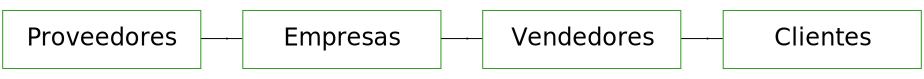
\includegraphics[width=150mm]{capitulos/graficos/cadenaAgentesPorter}
	\label{fig:cadenaAgentesPorter}

		\footnotesize
		Fuente: Brandenburguer y Harbone, 1996, p. 9.
\end{figure}



Por otro lado, el valor influye a la hora de llevar a cabo transacciones donde también se encuentran involucrados múltiples agentes de toda la cadena productiva y comercial, como son los proveedores, las empresas, los vendedores y como no, los clientes.  

En este sentido, el valor añadido se puede definir como el valor creado a lo largo del proceso, es decir, desde el vendedor hasta el consumidor, teniendo en cuenta la cantidad y el precio que están dispuestos a invertir en un producto o servicio que no sólo cubra las necesidades, si no también que aporte algún factor añadido (Brandenburguer y Harbone, 1996). La cadena de valor se puede representar verticalmente haciendo un recorrido por las acciones que desempeñan el comprador, la empresa y el proveedor. La parte inferior de la figura \ref{fig:cadenaValor}, representa la cantidad de valor que prosee el proveedor. En la parte central se encuentra el valor adquirido por la empresa, es decir, el precio recibido por el comprador menos el coste de los recursos por parte del proveedor. En la parte superior se representa la cantidad máxima que el comprador está dispuesto a pagar por un producto o servicio. El resultado que obtenga cada agente variará dependiendo de las armas con las que se lleven a cabo las negociaciones entre los compradores y la empresa; y entre la empresa y el proveedor. Algunos de estos elementos negociadores pueden ser la persistencia, las presiones o la paciencia.

\begin{figure}[!h]
	\caption{Cadena de valor}
	\centering 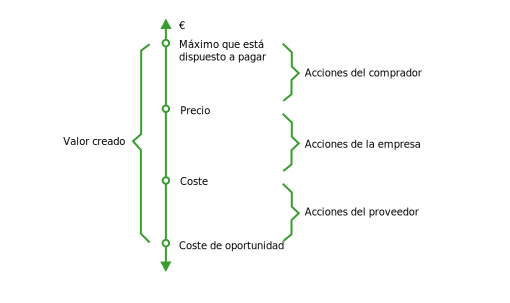
\includegraphics[width=150mm]{capitulos/graficos/cadenaValor}
	\label{fig:cadenaValor}

		\footnotesize
		Fuente: Brandenburguer y Harbone, 1996, p. 10
\end{figure}

Desde un punto de vista comercial, crear valor significa ofrecer algo a alguien que desea cubrir una necesidad y espera satisfacerla a cambio de un coste que generalmente es económico (Viscarri, 2011). Al mismo tiempo, este autor reflexiona que para las empresas cada vez es más complicado atender a todas las necesidades requeridas por los clientes ya que los mercados son cada vez más rigurosos y el entorno es cada vez más turbulento y sujeto a grandes presiones competitivas, legales, sociales y económicas. Para hacer frente a esta serie de sucesos son necesarios el esfuerzo y la integridad. Esfuerzo para mejorar e integridad para aproximarse a lo que el cliente espera, pero sin fraudes.

Sawhney (2003) establece siete fundamentos imprescindibles sobre el concepto de valor:

\begin{enumerate}
	\item \emph{El valor tiene que estar definido por el cliente}. Para Drucker (1993) lo más trascendente es lo que el cliente siente y piensa a la hora de comprar o disfrutar un bien o servicio, es decir, lo que para él tiene valor, restándose así importancia a lo que la empresa cree que tiene valor.
	\item \emph {El valor es opaco}. Las empresas tienen que realizar un ejercicio de empatía con los clientes, para poder “caminar en sus zapatos y sentir su dolor” (Drucker, 1993) (ver figura \ref{fig:empatiaMaegias}).
	\begin{figure}[!h]
	\caption{Mapa de empatía}
	\centering \includegraphics[width=110mm]{capitulos/graficos/empatiaMaegias}
	\label{fig:empatiaMaegias}

		\footnotesize
		Fuente: Megias, 2012
\end{figure}
	\item \emph {El valor es contextual}. El valor, se encuentra en los ojos, en las mentes y en los corazones de los clientes. Por lo tanto, es irrelevante hablar sobre el valor de un producto sin conocer el contexto en el que se desenvuelve la acción y sin tener en cuenta que los clientes son heterogéneos. El contexto tiene tres dimensiones importantes: el usuario final, la situación de uso final, y el medio ambiente (Drucker 1993).
	\item \emph {El valor es multidimensional} (Sawhney 2003; Lapierre, 2000):
		\begin{itemize}
			\item \emph{La dimensión funcional}. Es el valor de las características y funciones de un producto o servicio.
			\item \emph{La dimensión emocional}. Son los beneficios psicológicos que obtiene el cliente al comprar, usar, poseer o disfrutar el producto o servicio.
			\item  \emph{La dimensión económica}. Los clientes también evalúan el valor económico.

		\end{itemize}
	\item \emph{El valor es un trade-off}. Tras la lectura comprensiva de tres diccionarios monolingües\footnote{Merriam Webster, Oxford y Webster´s New World College Dictionary.}, se puede decir que trade-off es un tipo de intercambio de un producto o servicio donde el cliente le asigna un valor y lo intercambia por otro producto o servicio que valora en mayor medida. Por lo que se puede afirmar que valor es un trade-off entre el total de los beneficios que el cliente recibe y los costes totales en que incurre.
	\item \emph{El valor es relativo}. Antes de adquirir el producto o servicio, los clientes realizan una comparación entre toda la oferta de las diferentes compañías. Normalmente va a existir una alternativa a la empresa nodal\footnote{Compañía principal a estudiar o analizar.} a la que se le denomina el mejor sustituto disponible o equivalente (Sawhney, 2006), es decir, la opción que los usuarios elegirán si deciden prescindir de los servicios de esta compañía nodal
	\item \emph{El valor es un estado mental}. Para llevar a cabo una gestión basada en el valor hay que evaluar el modo de pensar de los clientes.

\end{enumerate}

Pese a que los autores no coinciden en numerosos aspectos, parece existir un consenso en que cuanta mayor intensidad tenga el papel del cliente en la creación de valor, mayor competitividad adquiere la empresa. A este marco de referencia de creación de valor conjunta se le ha denominado “co-creación de valor” (Vargo y Lusch, 2004).


\chapter{La co-creación de valor positiva o negativa para la empresa}
\label{anexo:2}

\section{El concepto de co-creación de valor positivo y negativo}

Según la teoría de Prahalad y Ramaswamy (2004), el valor se crea cuando los usuarios tienen una experiencia acumulada que viene proporcionada a través de los recursos, procesos y estados propuestos por la empresa y establecen así sus propios resultados. Dando como resultado, que el valor se realiza a través de la posesión, uso, o estados mentales del usuario. En este sentido la empresa deberá facilitar la co-creación de valor a los clientes y eso significa que la empresa ha de crear un valor potencial que el cliente puede transformar en el valor en uso o valor real. Retomando al autor Grönroos (2008), la co-creación de valor a través de la interacción en el consumo, hace que el cliente tenga sentimientos positivos, es decir, se siente mejor; o por el contrario sentimientos negativos, es decir, se siente peor. De este modo, surge la co-creación positiva o negativa con sus respectivas consecuencias para la empresa.

Aunque el concepto de experiencia acumulada de Prahalad y Ramaswamy, parece implicar un nivel constante de evolución positiva del valor, esto no ocurre en todos los casos. El proceso de acumulación de valor puede incluir tanto las experiencias positivas como las experiencias negativas de valor, donde a veces el cliente también puede llegar a ser un enemigo empresarial.

Para poder apreciar la diferencia entre una co-creación de valor positiva y negativa con más claridad, se van a exponer dos breves ejemplos prácticos. El primero de ellos es la empresa Hyve AG y la segunda es SPAR Austria.

\subsection{La co-creación de valor positiva}

Hyve AG es una conocida empresa de innovación con sede en Alemania. Su director, el Dr. Johann Fuller, afirma que el conocimiento acumulado y la creatividad, son el resultado de la interacción entre la empresa y el cliente y lo utilizan como un acelerador hacia la innovación, la mejora de la calidad del servicio y el refuerzo a la hora de retener clientes y fidelizarlos. Como consecuencia, también se puede conseguir una reducción de costes al largo plazo. La opinión de Fuller es que las empresas por si solas no pueden ofrecer propuestas de valor, y que por lo tanto son los consumidores los que crean el valor a través del uso y la aceptación del producto o servicio (Gebauer, Füller y Pezzei. 2012).

Hyve AG, ha desarrollado una plataforma Web\footnote{Hyve AG. (2015). HYVE Science Labs. Recuperado de \url{https://www.hyvescience.net/}} donde se realiza un intercambio de información entre la empresa y los usuarios. En esa página Web, la empresa comunica a los clientes las necesidades, los problemas y los retos a los que se están enfrentando. También proponen la participación de los usuarios en los proyectos. De esta forma, la empresa puede evaluar constantemente la relación del consumidor con sus productos para poder mejorar y personalizar los métodos ayudándoles a crecer como empresa y como comunidad. Por lo tanto, esta interacción se puede considerar positiva para la empresa.

\subsection{La co-creación de valor negativa}

La empresa SPAR Austria, una de las principales cadenas de distribución en Austria, creó un concurso llamado “SPAR Bag Design Contest”, traducido al castellano es “Concurso de bolsas de diseño SPAR”. Se trataba de un concurso internacional de diseño de bolsas de compra a través de la página Web del propio supermercado SPAR. El concurso invitaba a los aficionados al arte, estudiantes de diseño, diseñadores profesionales, etc. a presentar sus ideas mediante un programa informático añadido en su página Web\footnote{SPAR Österreich - Startpage. (2011). Recuperado de http://www.spar.at/de\_AT/index.html} y de fácil uso.

Tras la proclamación del ganador, la empresa tuvo que lidiar con el sentimiento de descontento de los usuarios que arremetieron contra la marca SPAR mediante quejas escritas en la página Web y comentarios negativos sobre los diseños ganadores. De este modo, los usuarios transformaron la página Web en una plataforma para expresar sus protestas. La razón principal del descontento era la decepción de los concursantes con el ganador elegido por el jurado. Se había elegido como ganador un diseño poco creativo en cuanto al diseño gráfico, pero muy ocurrente por su juego de palabras. De este modo, los participantes que no hablaban alemán no pudieron comprender ese juego de palabras. Aun así, estas reacciones negativas, proporcionaron información valiosa para SPAR sobre los factores desencadenantes de esta conducta por parte de los usuarios en las comunidades Web de innovación (Gebauer, Füller y Pezzei 2012).

Se puede afirmar, que si las expectativas del cliente no se cumplen, no surgirá el bienestar. De esta forma, la experiencia de consumo va acompañada de un efecto negativo que conduce a emociones como la ira, la frustración o la irritación. El comportamiento negativo de los consumidores puede desembocar en una conducta disfuncional de los clientes, término que se refiere a un comportamiento desviado por los clientes (Gebauer, Füller y Pezzei 2012). Los usuarios que intervienen de forma disfuncional, pueden causar serios problemas a la empresa, a los empleados e incluso a otros clientes. Esta conducta puede darse por motivos económicos, de situación o personales. Esta insatisfacción puede verse reflejada en un comportamiento de queja, realizar un boicot a la marca, actuar de manera fraudulenta o también puede que el cliente quiera sacar provecho haciendo una reclamación para recuperar un servicio gratuitamente. También es posible que se de abuso verbal o incluso físico a los empleados. Además los consumidores insatisfechos y que a su parecer no han recibido un trato justo por la empresa, también pueden llegar a ser clientes insatisfechos y activos realizando daño a la empresa mediante el boca a boca (WOM) negativo.

Pueden surgir también comunidades anti-marca. Existen multitud de éstas centradas en cuestiones ecológicas, ambientales, de derechos humanos, etc. Uno de los casos más llamativos es el que estudiaron los autores Thompson, Rindfleisch y Arsel (2006). Investigaron un fenómeno llamado el efecto Doppelgänger. Se trata de un término alemán que se usa para definir al doble fantasmagórico de una persona o cosa. En el caso de la figura \ref{fig:Starbucks}, lo que pretendía la organización de consumidores orgánicos era burlarse y poner en entre dicho a la marca Starbucks con el fin de perjudicar a la firma y ponerla en el punto de mira.

\begin{figure}[!h]
	\caption{Doppelgänger Starbucks}
	\centering 
\includegraphics[width=110mm]{capitulos/graficos/Starbucks}
	\label{fig:Starbucks}

		\footnotesize
		Fuente: adaptado de organicconsumers.org
\end{figure}

A modo resumen, se puede afirmar que no siempre las empresas consiguen los objetivos y el enfoque que pretendían en un principio con las medidas de co-creación de valor que diseñaron. No por ello, tienen que dejar de intentar co-crear valor, deberán reinventarse y seguir investigando otras vías que faciliten estos procesos de co-creación. En cuanto a la co-creación positiva, hay que señalar que el desarrollo de las nuevas tecnologías, de las Web 2.0 y de las plataformas engagement, ha favorecido la comunicación y el diálogo entre empresas y consumidores acercándoles cada vez más y ha facilitado la co-creación de valor.

\chapter{Ampliación del epígrafe \ref{section:procesosCocreacion}}
\label{anexo:3}

\section{El desarrollo de nuevos productos y/o servicios}
\subsection*{Los procesos de co-creación de valor como una oportunidad de desarrollo de nuevos productos y/o servicios}


Con este anexo, se quiere ofrecer una visión sobre el marco de actividades de co-creación de valor en los procesos de innovación empresariales. Este hecho implica la necesidad de pensar en la co-creación como un programa estratégico y no como un justo a tiempo de la externalización de las tareas de innovación (O'Hern y Rindfleisch, 2010).

Una de las características que hay que destacar del entorno de la innovación, es el reciente aumento en el contenido generado por el usuario, (CGU) y que está transformando radicalmente el panorama del marketing (Instituto de ciencia de marketing, 2008). O'Hern y Rindfleisch (2010), definen el contenido generado por el usuario como la contribución original que los usuarios aportan sobre un producto dirigido a otros usuarios, y/o el desarrollo de estos productos. Estas contribuciones proporcionan a los desarrolladores de productos de las empresas información valiosa sobre sobre el funcionamiento de un producto, cómo se puede mejorar, e incluso pueden aportar soluciones reales a los problemas relacionados con el producto.

En la actualidad es común encontrarse con un número creciente de consumidores muy bien informados y conectados y que ya no se contentan con la simple elección y uso de los productos y servicios de una empresa, sino que ellos también quieren contribuir al desarrollo y promoción de estos procesos. En los últimos años, un número creciente de académicos han comenzado a investigar el impacto del CGU en diversos campos del marketing (Chevalier y Mayzlin 2006; Godes y Mayzlin 2004), sugiriendo que el poder del CGU radica en su capacidad para llamar la atención sobre un producto y su promoción a través del boca a boca. Este término se concentra en la comunicación establecida entre consumidor y consumidor y considera al CGU como un vehículo para la promoción del producto (Godes y Mayzlin, 2004).

Retomando la teoría de O'Hern y Rindfleisch (2010), acerca de la investigación de innovación por parte del usuario, estos autores reconocen el papel activo que los usuarios adquieren en el proceso de co-creación considerándoles agentes de innovación. Un ejemplo antiguo pero claro es el de Raymond (1999) sobre los inicios de Linux. En esta empresa, tuvieron en cuenta los amplios conocimientos de sus usuarios para crear el código fuente de Linux y cuando los propios clientes encontraban fallos, los reportaban y propiciaban cambios que daban lugar a mejoras importantes. Por lo que, la innovación por parte del usuario crea contribuciones potenciales, nuevas ideas y soluciones.

Bartl (2006), establece un plan de acción a la hora de co-crear valor en productos o servicios innovadores, dando respuesta a cuándo, quién y cómo co-crear.

En lo que se refiere a la primera cuestión, Michael Bartl (2009) parte de la división del proceso de innovación en cinco fases:

\begin{enumerate}
	\item \emph{Oportunidades e ideas}.
	\item \emph{Conceptos}.
	\item \emph{El diseño y la ingeniería}.
	\item \emph{Pruebas}.
	\item \emph{Lanzamiento}.
\end{enumerate}

Normalmente, las empresas a la hora de co-crear centran principalmente sus objetivos en la participación de los clientes finales, consumidores o usuarios. Sin embargo, en algunos casos también se deberían de tener en cuenta a otros grupos de intermediarios como clientes corporativos, distribuidores, socios comerciales, instituciones gubernamentales o las asociaciones de consumidores. La duración y la estabilidad de la relación con el cliente depende de una diferenciación entre los clientes existentes, los latentes y los nuevos.

El desarrollo de las TIC, ha propiciado herramientas diseñadas para el cliente online. Un número cada vez mayor de usuarios están contribuyendo activamente a la creación de ideas y a proporcionar soluciones online. Estos usuarios online juegan un papel muy importante para las empresas porque expresan sus propias percepciones de la calidad del producto. En el caso de los clientes fieles, incluso pueden influir en las actividades de promoción de la competencia de la empresa realizando comentarios de desprestigio (Mayzlin, 2006). Un ejemplo es la campaña de XS desprestigiando la bebida austríaca Red Bull\footnote{Tejada, M, C. (2015). El nuevo diario. Recuperado de www.elnuevodiario.com.do/mobile/article.aspx?id=17531}.

Una de las cuestiones importantes de la co-creación de valor es establecer en qué etapa del proceso de innovación los clientes pueden tener una mayor participación, bien en la generación de ideas, en la evaluación y refinamiento de conceptos, en especificar las características del producto o en la creación de prototipos, etc. Por lo tanto, se puede decir que el consumidor puede ser de utilidad creativa influyendo en las tres primeras fases de Bart (2006), es decir, creando oportunidades e ideas, concretándolas y participando en el diseño o incluso en la ingeniería. Un ejemplo, son las páginas Web Dell IdeaStorm\footnote{Dell Idea Storm. (2015). Recuperado de www.ideastorm.com/} o Lego\footnote{LEGO.com Digital Designer Virtual Building Software. (2015). Recuperado de http://ldd.lego.com/en-us/}. Estas páginas Web se utilizan como un medio de comunicación entre los consumidores y los desarrolladores y se consideran como un mecanismo en el que los consumidores aportan ideas y soluciones que pueden influir directamente en la innovación de productos (O'Hern y Rindfleisch, 2010). Por otro lado, se encuentran los procesos por los que las empresas tienen un producto ya desarrollado y lo que pretenden es innovar a partir de ese producto base, como es el caso de BMW\footnote{Bilgram,V. (2010). Value Co-Creation: From Piloting to Continuous Co-Creation. Recuperado de http://value-co-creation.blogspot.co.at/2010/11/from-piloting-to-continuous-co-creation.html} y Nivea\footnote{Bilgram,V. (2011). Nivea's Co-Creation Process: the Case of the Invisible for Black \& White. Recuperado de http://www.slideshare.net/HYVE/2011-0228-nivea-invisible-for-black-white-deodorant}. En estos casos, el proceso de co-creación surge en las últimas etapas descritas por Bartl (2009), es decir, en los test y puesta en marcha del producto o servicio.

Otra idea que hay que señalar de Bartl (2009), es el grado de implicación de los usuarios para que participen en las actividades propuestas de co-creación. Hay dos vertientes:

\begin{enumerate}
	\item \emph{La motivación intrínseca}.
	\item \emph{La motivación extrínseca}.
\end{enumerate}

La motivación intrínseca de los clientes es el hecho de realizar una acción para satisfacer una necesidad y sentirse motivado al llevarla a cabo por un aspecto separable, es decir, cuando una persona se encuentra motivada intrínsecamente, actúa con una finalidad lúdica y no suele encontrarse motivada por agentes externos, o por sentirse presionada o por una posible recompensa futura. En cambio, la motivación extrínseca se da cuando el consumidor se ve motivado por las recompensas externas, bien sean intereses económicos, o recompensas. (Ryan y Deci, 2000). Para poder comprender estos dos términos, se van a citar algunos ejemplos. La motivación intrínseca es palpable en los niños pequeños porque tratan constantemente de agarrar, tirar, morder o gritar a los objetos nuevos que se encuentran para poder obtener información de ellos. A medida que estos niños van creciendo, el entorno les hace seguir estando intrínsecamente motivados a través de crucigramas, de la lectura de novelas o incluso del hecho de ver películas. Por otro lado, algunos casos de la motivación extrínseca pueden llevarse a cabo mediante recompensas externas, como por ejemplo dinero o ascensos en los puestos de trabajo (Bartl 2009).

Retomando el caso de los consumidores, los usuarios que estén motivados intrínsecamente valorarán el intercambio comercial de una forma muy intensa, sin embargo, si están motivados extrínsecamente sólo se centrarán en los resultados. Por lo tanto, algunas de las motivaciones intrínsecas que puede tener el consumidor son: la curiosidad, la auto eficacia, el desarrollo de actividades, la búsqueda de información, la necesidad personal, etc. La motivación intrínseca destaca en los clientes altamente involucrados y que ayudan en mayor medida al proceso de co-creación de valor. No obstante, cuando las empresas buscan co-crear con los usuarios en productos innovadores, la motivación deberá ser intrínseca y extrínseca, ya que tienen que tienen que exponer el 100\% de sus ideas teniendo en cuenta sus motivaciones y manifestar los resultados finales que quieren obtener.

Por lo tanto, un programa de co-creación de valor en productos innovadores, debe estar caracterizado por una relación de colaboración continua entre la empresa y los usuarios. Esta relación se describe de una forma gráfica en la figura \ref{fig:cocreacionInnovacionBartl}. Las interacciones entre la compañía y los clientes deben darse a lo largo del proceso de innovación y las ideas que se desarrollen tienen que concordar con los límites y los resultados de la organización.

\begin{figure}[!h]
	\caption{Enfoque programático para la formación de co-creación continua}
	\centering \includegraphics[width=140mm]{capitulos/graficos/cocreacionInnovacionBartl}
	\label{fig:cocreacionInnovacionBartl}

		\footnotesize
		Fuente: Bartl, 2010
\end{figure}

Como se puede apreciar en la figura \ref{fig:cocreacionInnovacionBartl}, pueden existir diferentes procesos de co-creación, representados con los círculos en forma de flechas, en un mismo momento del desarrollo del producto. Las flechas indican la necesidad no sólo de buscar y adquirir innovación, sino también asimilar y explotar esta entrada dentro de todos los procesos siguientes.

A su vez, estos procesos co-creativos de innovación pueden estar más o menos abiertos, representados a través de los diferentes tonos de grises. Cuanta mayor intensidad tenga el tono gris, querrá decir que ese proceso de co-creación es cerrado. Un ejemplo de ello pueden ser los blogs que facilitan las actualizaciones del proyecto, la organización, la comunicación con el cliente, etc. También, las redes sociales pueden proporcionar recursos desconocidos, mayor accesibilidad de los clientes a la empresa, datos de contacto, etc. Ambos forman parte de una amplia lista de elementos de un proceso cerrado de co-creación y es una forma rápida de conectar las opiniones y las visiones de los consumidores con la empresa. En cambio, cuanto menor intensidad tenga el color gris, el proceso de co-creación es más abierto, lo que supone que los clientes se involucren en mayor medida. Por ejemplo, en el año 2006 los fans de Doritos diseñaron sus propios anuncios para tener la oportunidad de ganar un viaje para ver en directo la Super Bowl. Otro ejemplo, como se ha señalado anteriormente, es la empresa Lego que cuenta con un sitio web donde invita a desarrollar ideas y proyectos a sus seguidores con la opción de poder fabricarlos en un futuro. La empresa también tiene que ser consciente de que los usuarios han de adaptarse a las herramientas que ésta les proporciona y de delimitar los límites hasta los que pueden involucrarse en el proceso de la co-creación, o por el contrario indicar a sus consumidores que no existen límites porque el proceso de co-creación es totalmente abierto. Por ejemplo, los círculos más cerrados, los grises, pueden ser herramientas enterprise 2.0; y los círculos más abiertos, los blancos, pueden ser plataformas crowdsourcing.

Para poder comprender estos términos, se ha de mencionar en primer lugar que el concepto de Web 2.0 y sus dinámicas de funcionamiento, hacen que se desemboque en el concepto de enterprise 2.0. Enterprise 2.0 es a la utilización por parte de las empresas, clientes y socios, del uso de plataformas software para la difusión de noticias, concursos, experiencias, etc. Las empresas que proponen este tipo de software a disposición de sus clientes, han sufrido una modificación de valores empresariales porque consideran a estas plataformas como software social, ya que disponen de las características y las funciones necesarias para cubrir las necesidades de la sociedad. Algunos ejemplos de entidades que utilizan estas herramientas para crear contenido son Flickr, Google, Wikipedia, etc (Forbes, 2010). Por otro lado, las plataformas Crowdsourcing son un nuevo modelo de negocio que se utiliza para externalizar de forma distribuida las tareas de la empresa. También se utiliza para poder crear ideas y solucionar problemas comunes entre todos los agentes.

\begin{figure}[!h]
	\caption{La co-creación en proyectos de innovación}
	\centering 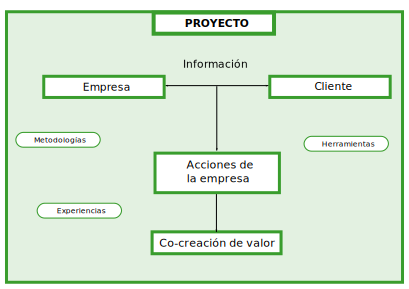
\includegraphics[width=140mm]{capitulos/graficos/proyectoInnovacionBartl}
	\label{fig:proyectoInnovacionBartl}

		\footnotesize
		Fuente: adaptado de Bartl, 2009
\end{figure}

Con todo lo explicado anteriormente, se puede decir que el éxito de la co-creación en proyectos de innovación depende de tres factores fundamentales (ver figura \ref{fig:proyectoInnovacionBartl}). En primer lugar, la excelencia del proyecto en términos metodológicos, las herramientas y las experiencias que la empresa debe de cumplir. En segundo lugar, diseñar un proceso de co-creación de valor continuo, creando un proceso interactivo entre los consumidores y la empresa. Y por último, las estructuras y las capacidades de la organización que tienen que establecerse con el fin de no ser sólo informaciones que den los usuarios si no que tengan como finalidad llevar a cabo mejores productos orientados hacia el cliente y aprovechar la co-creación de valor dentro de la empresa (Bartl, 2009).


\chapter{Ampliación del epígrafe \ref{section:logicasDominantes}}
\label{anexo:4}

\section{De la lógica dominante del producto a la lógica dominante del servicio}

Cómo se ha podido observar en la figura \ref{fig:evolucion} del capítulo \ref{section:cocreacion}, en 1960 nacen tres nuevos enfoques surgidos de la LDP (Vargo y Lusch, 2008):

\begin{itemize}
	\item \emph{El business to business (B2B)}. Se trata de la necesidad empresarial de abordar temas tales como el marketing industrial, la incapacidad de comercializar con ciertos productos, la incomprensión por parte de la LDP del concepto de intercambio, etc. De este modo nació el B2B.
	\item \emph{Marketing de servicios}. Cuyas diferencias básicas con la LDP son las siglas IHIP: Inseparabilidad de la producción y consumo, heterogeneidad, inventariabilidad y servicios perecederos. Por lo que las compañías tienen que ajustarse a estas diferencias. También, los investigadores comenzaron a encontrar alternativas como las relaciones en las transacciones, la calidad percibida por el cliente en lugar de tener en cuenta la marca entre otros.
	\item \emph{La teoría de la intersección}. Tiene su base en la reconceptualización del marketing, de producir bienes a producir algo más que servicios. Por ejemplo, en aerolíneas, bancos, salud, hoteles, etc., se ha de cambiar el concepto de producción de unidades de servicios a producir servicio. Vargo y Lusch (2008) afirman que el surgimiento de la LDS surge de esta rama.
\end{itemize}

\chapter{Aplicación de la lógica del servicio}
\label{anexo:5}

A continuación se exponen los 11 puntos que Grönroos (2006) ha desarrollado acerca de la lógica del servicio y su postura hacia el autoservicio.


\section{Las proposiciones de Grönroos (2006) relacionadas con la creación de valor y el autoservicio:}

\begin{itemize}
	\item La LS apoya la creación de valor para los clientes por sí solos mediante el autoservicio.
	\item En el autoservicio también se puede co-crear valor. Los bienes y servicios han sido adquiridos por los clientes, junto con otros recursos necesarios que son utilizados por los clientes como recursos de entrada y los usuarios han de desarrollar su conocimiento y habilidad.
	\item Teniendo en cuenta el caso anterior, mediante el uso de estos recursos y la aplicación de esos conocimientos en el proceso de generación de valor en el autoservicio, los clientes van a crear valor para ellos mismos.
	\item La empresa por si sola no puede crear valor para los clientes. Su función es ser \emph{facilitadora} de valor, es decir, proporciona a los clientes los productos y servicios necesarios para facilitar los procesos de generación de valor en el autoservicio. Por lo tanto, se puede decir que la empresa está indirectamente involucrada con los clientes en la creación de valor.
	\item Y por último, otra de las funciones de la empresa, es la creación de oportunidades para desarrollar las interacciones con sus clientes durante sus procesos de generación de valor. Este hecho, provoca el cumplimiento de valor para los clientes y por lo tanto se convierten en co-creadores de valor.
\end{itemize}

\section{Las proposiciones relacionadas con la oferta del mercado:}

\begin{itemize}
	\item Ha de surgir el apoyo a los recursos, tales como bienes, servicios, información e interacciones entre el cliente y la empresa en el proceso de creación de valor de los propios clientes. La propuesta de co-creación de valor se produce gracias a la interacción entre ambos.
	\item Los clientes utilizan los bienes y servicios para producir un servicio por si solos que crea valor para ellos.
	\item La adopción de la LS es una decisión estratégica. Si los clientes no están comprando los bienes y servicios, la empresa puede persuadirlos.

\end{itemize}

\section{Las proposiciones relacionadas con el marketing:}

\begin{itemize}
	\item La aplicación de la LS significa que la empresa no se limita a hacer propuestas de valor único, sino que también recibe oportunidades. Por ejemplo, través de las posibilidades de co-creación de valor durante las interacciones con los clientes. De este modo, la empresa participa activa y directamente en la co-creación de valor para sus clientes.
	\item En la LS, la interacción en el momento del intercambio es la base de la comercialización, es decir, el cambio no se orienta hacia la creación de valor de los clientes, sino hacia las transacciones y hacia la facilitación del valor.

\end{itemize}

\chapter{Concepto de walmartización}
\label{anexo:6}

La walmartización es un concepto moderno con el que Prahalad y Ramaswamy (2004) pretenden explicar porqué las empresas han de poner todos los medios de los que disponen para que el cliente se sienta lo suficientemente cómodo a la hora del intercambio y pueda crear valor a través de la experiencia. Según el diccionario Collins, la walmartización se produce cuando una gran empresa o cadena de empresas se mueven de una región a otra y devasta/n a las empresas locales. Además, estas empresas impulsan a los trabajadores a desplazarse y a percibir una renta más baja. Por lo tanto, teniendo en cuenta este concepto, la globalización, la desregulación, la externalización y la convergencia de las industrias, y las tecnologías están haciendo que sea más difícil diferenciar las ofertas. Esto quiere decir, que los productos y los servicios se enfrentan a la mercantilización. La mercantilización se da cuando las empresas son eficientes pero los consumidores no aprecian ninguna diferencia entre si van o no a comprar de forma inteligente y barata.

\chapter{Cuestionario clientes}
\label{anexo:7}

\section*{Instrucciones}

El cuestionario consta de 36 preguntas y es de tipo mixto. Usted deberá responder con la máxima sinceridad posible y de una forma subjetiva. En cada pregunta tiene la oportunidad de exponer sus ideas, quejas o valoraciones.

El cuestionario está dividido en dos partes. La primera, es un cuestionario tipo Likert en el que deberá de elegir el número que mejor se adapte a sus experiencias vividas a lo largo de su estancia en este hotel. La escala es la siguiente:

\begin{enumerate}
	\item Muy insatisfecho.
	\item Insatisfecho.
	\item Ni satisfecho ni insatisfecho.
	\item Satisfecho.
	\item Muy satisfecho.

	\end{enumerate}
El segundo cuestionario es de tipo dicotómico en el que sólo hay dos posibilidades: si y no. A su vez, este cuestionario está subdividido en apartados.

\section*{Parte 1}
Responda desde muy insatisfecho (1) a muy satisfecho (5):

\begin{enumerate}
	\item ¿Su reserva antes de llegar al hotel fue gestionada eficientemente?
	\item ¿Cómo fue su experiencia durante el check in?
	\item ¿Cómo fue su experiencia global con la habitación?
	\item ¿Qué le pareció la cama?
	\item ¿Está satisfecho con el baño de la habitación?
	\item ¿Está satisfecho con las amenidades del baño y los productos de aseo que el hotel le proporcionó?
	\item ¿Cómo evalúa la atención al huésped en general?
	\item ¿Está satisfecho con el servicio de desayunos?
	\item ¿Cómo evalúa los servicios de Internet y WiFi en el hotel?
	\item ¿Cómo ha sido el trato recibido por parte de los empleados a lo largo del check out?
	\item ¿Cómo ha sido la actitud y proactividad de los empleados durante su estancia en el hotel?
	\item ¿Qué le pareció la atmósfera del hotel (música, aroma, iluminación, decoración, mobiliario)?
	\item ¿Le parece adecuado el plan de fidelización que propone el hotel?
	\item ¿Cómo fue su experiencia global en el hotel?
	\item ¿Sintió que le mimamos durante su estancia?
	\item Cómo evalúa la relación calidad – precio global?
	\item ¿Volverá a este hotel?
	\item ¿Recomendará este hotel?
	\item ¿Cómo evaluaría el minibar de la habitación?
	\item ¿Cómo evaluaría la tintorería y el servicio de limpieza en seco?
	\item ¿Está satisfecho con el servicio durante la comida?
	\item ¿Está satisfecho con el servicio durante la cena?
	\item ¿Cómo evaluaría su experiencia en el bar?
	\item ¿Cómo evaluaría su experiencia en el gimnasio?
	\item ¿Cómo evaluaría el servicio de habitaciones?

\end{enumerate}

\section*{Parte 2}
Responda si/no.


\subsection*{Participación}
\begin{enumerate}
	\item ¿Promueve la oferta cultural de la ciudad de Viena?
	\item ¿Proporciona usted productos y servicios sostenibles a otros huéspedes?
	\item ¿Apoya a las actividades de las ONGs o de otras organizaciones locales?
	\item ¿Administra los recursos naturales de una forma responsable (agua, energía, desperdicios)?
	\item ¿Contribuye al desarrollo económico de este hotel con su estancia?
	\item ¿Le gustaría enviar su opinión a Tripadvisor a través de esta encuesta?

\end{enumerate}

\subsection*{Problemas}
\begin{enumerate}
	\item ¿Tuvo algún problema?
	\item ¿Reportó ese problema?

\end{enumerate}

\subsection*{Fidelización}
\begin{enumerate}
	\item Durante su estancia, ¿le informaron sobre los beneficios del programa de fidelidad?
	\item ¿Es miembro del programa de fidelidad?
	\item ¿Se hizo miembro del programa de fidelidad durante la última estancia?

\end{enumerate}

Los ítems número: 19, 20, 21, 22, 23, 24 y 25 que son de tipo Likert, han sido eliminados del estudio debido a la escasez de respuestas o a la escasez de fiabilidad que aportaban según el análisis factorial realizado. Por lo tanto, el contraste de hipótesis se ha llevado a cabo con un total de 29 ítems divididos en 6 factores.

\chapter{Resultados SPSS del estudio 1. Análisis factorial}
\label{anexo:8}

\begin{table}[h]
    \caption {Prueba de KMO y Bartlett del estudio 1}
	\label{tab:kmo1}
	\setlength\extrarowheight{5pt}
	
	\begin{tabular}{p{5.7cm} p{4.6cm} p{2.8cm}}
	\toprule
	\multicolumn{2}{c}{Medida de adecuación de muestra de Kaiser-Meyer-Olkin}	& 0,611 \\
									& Chi-Cuadrado aprox	& 462,649 \\
	Test de esfericidad de Bartlett	& Desviación estándar					& 153 \\
									& Significación					& 0.000 \\
	\bottomrule
	\end{tabular}
	
	\center
	\footnotesize
	Fuente: elaboración propia
\end{table}


\begin{figure}[!h]
	\caption{Gráfico de sedimentación}
	\centering \includegraphics[width=150mm]{capitulos/graficos/sedimentacion}
	\label{fig:sedimentacion}

		\footnotesize
		Fuente: elaboración propia
\end{figure}

\newpage

\begin{table}[h]
    \caption {Varianza total explicada estudio 1}
	\label{tab:varianzaExplicada1}
	\setlength\extrarowheight{5pt}
	
	\begin{tabular}{p{1.5cm} p{1.9cm} p{1.7cm} p{1.7cm} p{1.9cm} p{1.9cm} p{1.7cm}}
	\toprule
	Comp.	& \multicolumn{3}{c}{Valores propios iniciales} & \multicolumn{3}{c}{Rotación de las sumas de los cuadrados} \\
	\midrule
		& Total	& \% de varianza	& \% acumulado	& Total	& \% de varianza 	& \% acumulado \\
	\midrule
	1  & 8,042 & 44,680 & 	44,680 & 5,059 & 28,106 & 28,106 \\
	2  & 2,285 & 12,697 & 	57,376 & 4,054 & 22,524 & 50,629 \\
	3  & 1,648 & 9,157 &	66,534 & 2,863 & 15,904 & 66,534 \\
	4  & 1,176 & 6,534 &	73,068 &  &  &  \\
	5  & 0,934 & 5,188 &	78,256 &  &  &  \\
	6  & 0,835 & 4,638 &	82,894 &  &  &  \\
	7  & 0,711 & 3,952 &	86,846 &  &  &  \\
	8  & 0,560 & 3,112 &	89,958 &  &  &  \\
	9  & 0,516 & 2,866 &	92,823 &  &  &  \\
	10 & 0,304 & 1,689 & 	94,513 &  &  &  \\
	11 & 0,259 & 1,437 & 	95,949 &  &  &  \\
	12 & 0,219 & 1,217 & 	97,166 &  &  &  \\
	13 & 0,185 & 1,028 & 	98,194 &  &  &  \\
	14 & 0,125 & 0,692 & 	98,886 &  &  &  \\
	15 & 0,110 & 0,611 & 	99,498 &  &  &  \\
	16 & 0,050 & 0,277 & 	99,775 &  &  &  \\
	17 & 0,025 & 0,138 & 	99,913 &  &  &  \\
	18 & 0,016 & 0,087 & 	100,000 &  &  &  \\
	\bottomrule
	\end{tabular}
	
	\center
	\footnotesize
	Método de extracción: Análisis del componente principal.\\
	Fuente: elaboración propia
\end{table}


\newpage

\begin{table}[h]
    \caption {Matriz de componentes rotados}
	\label{tab:componentes1}
	\setlength\extrarowheight{5pt}
	
	\begin{tabular}{p{7.0cm} p{2.3cm} p{2.3cm} p{1.5cm}}
	\toprule
		& \multicolumn{3}{c}{Componentes} \\
		& 1	& 2	& 3	\\
	\midrule
	Recomendar hotel & 0,872 &  & \\
	Desayuno & 0,812 &  & \\
	Amenidades baño & 0,762 &  & \\
	Calidad-precio & 0,722 &  & \\
	Volver hotel & 0,720 &  & \\
	Baño & 0,706 &  & \\
	Experiencia global hotel &  & 0,606 & \\
	Check in &  & 0,760 & \\
	Cama &  & 0,725 & \\
	Experiencia global habitación &  & 0,687 & \\
	Atmósfera hotel &  & 0,651 & \\
	Reserva gestionada bien &  & 0,645 & \\
	Atención al huésped &  & 0,599 & \\
	WiFi	&	& 0,458	&	\\
	Check out &  &  & 0,821 \\
	Proactividad empleados &  &  & 0,707 \\
	Mimos	&	&	&	0,615 \\
	Fidelidad	&	&	& 0,568 \\
	\bottomrule
	\end{tabular}
	
	\center
	\footnotesize
	Método de extracción: Análisis del componente principal.\\
	Método de rotación: Varimax con normalización de Kaiser.\\
	Fuente: elaboración propia
\end{table}


A continuación se muestran los nombres utilizados para nombrar a las variables en SPSS con sus respectivas preguntas.

\begin{itemize}
	\item \emph{Reserva gestionada bien.} ¿Su reserva antes de llegar al hotel fue gestionada eficientemente?
	\item \emph{Check in.} ¿Cómo fue su experiencia durante el checkin?
	\item \emph{Experiencia global habitación.} ¿Cómo fue su experiencia global con la habitación?
	\item \emph{Cama.} ¿Qué le pareció la cama?
	\item \emph{Baño.} ¿Está satisfecho con el baño de la habitación?
	\item \emph{Amenidades baño.} ¿Está satisfecho con las amenidades del baño y los productos de aseo que el hotel le proporcionó?
	\item \emph{Atención al huesped.} ¿Cómo evalúa la atención al huésped en general?
	\item \emph{Desayuno.} ¿Está satisfecho con el servicio de desayunos?
	\item \emph{WiFi.} ¿Cómo evalúa los servicios de Internet y WiFi en el hotel?
	\item \emph{Check out.} ¿Cómo ha sido el trato recibido por parte de los empleados a lo largo del check out?
	\item \emph{Proactividad empleados.} ¿Cómo ha sido la actitud y proactividad de los empleados durante su estancia en el hotel?
	\item \emph{Atmósfera hotel.} ¿Qué le pareció la atmósfera del hotel (música, aroma, iluminación, decoración, mobiliario)?
	\item \emph{Experiencia global hotel.} ¿Cómo fue su experiencia global en el hotel?
	\item \emph{Mimos.} ¿Sintió que le mimamos durante su estancia?
	\item \emph{Calidad-precio.} Cómo evalúa la relación calidad – precio global?
	\item \emph{Volver hotel.} ¿Volverá a este hotel?
	\item \emph{Recomendar hotel.} ¿Recomendará este hotel?
	\item \emph{Fidelidad.} ¿Le parece adecuado el plan de fidelización que propone el hotel?
\end{itemize}

\chapter{Resultados SPSS del estudio 1. Aceptación y fiabilidad de los factores}
\label{anexo:9}

\section{Factor co-creación}

\begin{table}[h]
    \caption {Prueba de KMO y Bartlett de la co-creación}
	\label{tab:kmo2}
	\setlength\extrarowheight{5pt}
	
	\begin{tabular}{p{5.7cm} p{4.6cm} p{2.8cm}}
	\toprule
	\multicolumn{2}{c}{Medida de adecuación de muestra de Kaiser-Meyer-Olkin}	& 0,665 \\
									& Chi-Cuadrado aprox	& 76,793 \\
	Test de esfericidad de Bartlett	& Desviación estándar					& 6 \\
									& Significación					& 0.000 \\
	\bottomrule
	\end{tabular}
	
	\center
	\footnotesize
	Fuente: elaboración propia
\end{table}


\begin{table}[h]
    \caption {Estadísticas de fiabilidad de la co-creación}
	\label{tab:fiabilidadCocreacion}
	\setlength\extrarowheight{5pt}
	
	\begin{tabular}{p{5.7cm} p{4.6cm} p{2.8cm}}
	\toprule
	Alfa de Cronbach	& Alfa de Cronbach basada en elementos estandarizados	& Nº de elementos \\
	\midrule
	0,837				& 0,852					& 6 \\
	\bottomrule
	\end{tabular}
	
	\center
	\footnotesize
	Fuente: elaboración propia
\end{table}


\begin{table}[h]
    \caption {Varianza total explicada de la co-creación de valor}
	\label{tab:varianzaExplicada2}
	\setlength\extrarowheight{5pt}
	
	\begin{tabular}{p{1.5cm} p{1.9cm} p{1.7cm} p{1.7cm} p{1.9cm} p{1.9cm} p{1.7cm}}
	\toprule
	Comp.	& \multicolumn{3}{c}{Valores propios iniciales} & \multicolumn{3}{c}{Rotación de las sumas de los cuadrados} \\
	\midrule
		& Total	& \% de varianza	& \% acumulado	& Total	& \% de varianza 	& \% acumulado \\
	\midrule
	1	& 2,511	& 62,785	& 62,785	& 2,511	& 62,785	& 62,785 \\
	2	& 0,723	& 18,075	& 80,860	& 	& 	&  \\
	3	& 0,502	& 12,557	& 93,417	& 	& 	&  \\
	4	& 0,263	& 6,683		& 100,000	& 	& 	&  \\
	\bottomrule
	\end{tabular}
	
	\center
	\footnotesize
	Método de extracción: Análisis del componente principal.\\
	Fuente: elaboración propia
\end{table}


\begin{table}[h]
    \caption {Matriz de componentes co-creación}
	\label{tab:componentes2}
	\setlength\extrarowheight{5pt}
	
	\begin{tabular}{p{8.0cm} p{4.3cm}}
	\toprule
		& Componente 1 \\
	\midrule
	Proactividad empleados & 0,821 \\
	Check out & 0,808 \\
	Mimos & 0,817 \\
	Fidelidad & 0,719 \\
	\bottomrule
	\end{tabular}
	
	\center
	\footnotesize
	Método de extracción: Análisis del componente principal.\\
	Método de rotación: Varimax con normalización de Kaiser.\\
	Fuente: elaboración propia
\end{table}


\section{Factor satisfacción}

\begin{table}[h]
    \caption {Prueba de KMO y Bartlett de la satisfacción}
	\label{tab:kmo1}
	\setlength\extrarowheight{5pt}
	
	\begin{tabular}{p{5.7cm} p{4.6cm} p{2.8cm}}
	\toprule
	\multicolumn{2}{c}{Medida de adecuación de muestra de Kaiser-Meyer-Olkin}	& 0,812 \\
									& Chi-Cuadrado aprox	& 184,386 \\
	Test de esfericidad de Bartlett	& Desviación estándar					& 15 \\
									& Significación					& 0.000 \\
	\bottomrule
	\end{tabular}
	
	\center
	\footnotesize
	Fuente: elaboración propia
\end{table}


\input{./capitulos/tablas/fiabilidadSatisfaccion.tex}

\newpage

\begin{table}[h]
    \caption {Varianza total explicada de la satisfacción}
	\label{tab:varianzaExplicadaS}
	\setlength\extrarowheight{5pt}
	
	\begin{tabular}{p{1.5cm} p{1.9cm} p{1.7cm} p{1.7cm} p{1.9cm} p{1.9cm} p{1.7cm}}
	\toprule
	Comp.	& \multicolumn{3}{c}{Valores propios iniciales} & \multicolumn{3}{c}{Rotación de las sumas de los cuadrados} \\
	\midrule
		& Total	& \% de varianza	& \% acumulado	& Total	& \% de varianza 	& \% acumulado \\
	\midrule
	1  & 3,468 & 57,798 & 	57,798 & 3,468 & 57,798 & 57,798 \\
	2  & 0,837 & 13,945 & 	13,945 & &  &  \\
	3  & 0,611 & 10,181 &	10,181 & &  &  \\
	4  & 0,518 & 8,634 &	8,634 &  &  &  \\
	5  & 0,323 & 5,382 &	5,382 &  &  &  \\
	6  & 0,244 & 4,060 &	4,060 &  &  &  \\
	\bottomrule
	\end{tabular}
	
	\center
	\footnotesize
	Método de extracción: Análisis del componente principal.\\
	Fuente: elaboración propia
\end{table}


\begin{table}[h]
    \caption {Matriz de componentes de la satisfacción}
	\label{tab:componentesS}
	\setlength\extrarowheight{5pt}
	
	\begin{tabular}{p{8.0cm} p{4.3cm}}
	\toprule
		& Componente 1 \\
	\midrule
	Recomendar hotel & 0,862 \\
	Volver hotel & 0,732 \\
	Baño & 0,802 \\
	Amenidades baño & 0,770 \\
	Calidad-precio & 0,686 \\
	Desayuno & 0,694 \\
	
	\bottomrule
	\end{tabular}
	
	\center
	\footnotesize
	Método de extracción: Análisis del componente principal.\\
	Método de rotación: Varimax con normalización de Kaiser.\\
	Fuente: elaboración propia
\end{table}


\newpage

\section{Factor bienestar}

\begin{table}[h]
    \caption {Prueba de KMO y Bartlett del bienestar}
	\label{tab:kmoB}
	\setlength\extrarowheight{5pt}
	
	\begin{tabular}{p{5.7cm} p{4.6cm} p{2.8cm}}
	\toprule
	\multicolumn{2}{c}{Medida de adecuación de muestra de Kaiser-Meyer-Olkin}	& 0,814 \\
									& Chi-Cuadrado aprox	& 209,552 \\
	Test de esfericidad de Bartlett	& Desviación estándar					& 28 \\
									& Significación					& 0.000 \\
	\bottomrule
	\end{tabular}
	
	\center
	\footnotesize
	Fuente: elaboración propia
\end{table}


\begin{table}[h]
    \caption {Prueba de KMO y Bartlett del bienestar}
	\label{tab:fiabilidadBienestar}
	\setlength\extrarowheight{5pt}
	
	\begin{tabular}{p{5.7cm} p{4.6cm} p{2.8cm}}
	\toprule
	Alfa de Cronbach	& Alfa de Cronbach basada en elementos estandarizados	& Nº de elementos \\
	\midrule
	0,763				& 0,801					& 4 \\
	\bottomrule
	\end{tabular}
	
	\center
	\footnotesize
	Fuente: elaboración propia
\end{table}


\begin{table}[h]
    \caption {Varianza total explicada del bienestar}
	\label{tab:varianzaExplicadaB}
	\setlength\extrarowheight{5pt}
	
	\begin{tabular}{p{1.5cm} p{1.9cm} p{1.7cm} p{1.7cm} p{1.9cm} p{1.9cm} p{1.7cm}}
	\toprule
	Comp.	& \multicolumn{3}{c}{Valores propios iniciales} & \multicolumn{3}{c}{Rotación de las sumas de los cuadrados} \\
	\midrule
		& Total	& \% de varianza	& \% acumulado	& Total	& \% de varianza 	& \% acumulado \\
	\midrule
	1  & 3,886 & 48,574 & 	48,574 & 3,886 & 48,574 & 48,574 \\
	2  & 1,010 & 12,628 & 	61,202 &  &  &  \\
	3  & 0,901 & 11,265 &	72,467 &  &  &  \\
	4  & 0,652 & 8,146 &	80,613 &  &  &  \\
	5  & 0,612 & 7,650 &	88,264 &  &  &  \\
	6  & 0,396 & 4,951 &	93,215 &  &  &  \\
	7  & 0,297 & 3,719 &	96,933 &  &  &  \\
	8  & 0,245 & 3,067 &	100,000 &  &  &  \\
	\bottomrule
	\end{tabular}
	
	\center
	\footnotesize
	Método de extracción: Análisis del componente principal.\\
	Fuente: elaboración propia
\end{table}


\begin{table}[h]
    \caption {Matriz de componentes del bienestar}
	\label{tab:componentesB}
	\setlength\extrarowheight{5pt}
	
	\begin{tabular}{p{8.0cm} p{4.3cm}}
	\toprule
		& Componente 1 \\
	\midrule
	Experiencia global hotel & 0,852 \\
	Experiencia global habitación & 0,654 \\
	Atmósfera hotel & 0,667 \\
	Cama & 0,488 \\
	Check in & 0,774 \\
	WiFi & 0,649 \\
	Atención al huésped & 0,746 \\
	Reserva gestionada bien & 0,698 \\
	\bottomrule
	\end{tabular}
	
	\center
	\footnotesize
	Método de extracción: Análisis del componente principal.\\
	Método de rotación: Varimax con normalización de Kaiser.\\
	Fuente: elaboración propia
\end{table}



\chapter{Resultados SPSS del estudio 2. Aceptación y fiabilidad de los factores}
\label{anexo:10}
\section{Factor participación}

\begin{table}[h]
    \caption {Estadísticas de fiabilidad de la participación}
	\label{tab:fiabilidadParticipacion}
	\setlength\extrarowheight{5pt}
	
	\begin{tabular}{p{5.7cm} p{4.6cm} p{2.8cm}}
	\toprule
	Alfa de Cronbach	& Alfa de Cronbach basada en elementos estandarizados	& Nº de elementos \\
	\midrule
	0,701				& 0,827					& 6 \\
	\bottomrule
	\end{tabular}
	
	\center
	\footnotesize
	Fuente: elaboración propia
\end{table}


\section{Factor problemas}
\begin{table}[h]
    \caption {Estadísticas de fiabilidad de los problemas}
	\label{tab:fiabilidadProblemas}
	\setlength\extrarowheight{5pt}
	
	\begin{tabular}{p{5.7cm} p{4.6cm} p{2.8cm}}
	\toprule
	Alfa de Cronbach	& Alfa de Cronbach basada en elementos estandarizados	& Nº de elementos \\
	\midrule
	0,682				& 0,786					& 2 \\
	\bottomrule
	\end{tabular}
	
	\center
	\footnotesize
	Fuente: elaboración propia
\end{table}


\section{Factor fidelización}
\begin{table}[h]
    \caption {Estadísticas de fiabilidad de la fidelización}
	\label{tab:fiabilidadFidelizacion}
	\setlength\extrarowheight{5pt}
	
	\begin{tabular}{p{5.7cm} p{4.6cm} p{2.8cm}}
	\toprule
	Alfa de Cronbach	& Alfa de Cronbach basada en elementos estandarizados	& Nº de elementos \\
	\midrule
	0,734				& 0,851					& 3 \\
	\bottomrule
	\end{tabular}
	
	\center
	\footnotesize
	Fuente: elaboración propia
\end{table}


\chapter{Resultados SPSS del estudio. Contraste de hipótesis. ANOVA}
\label{anexo:11}

Hipótesis 1. Existe una relación directa entre la co-creación de valor y la satisfacción del cliente en el hotel.

\begin{table}[h]
    \caption {Resultados ANOVA para la hipótesis 1}
	\label{tab:anovaH1}
	\setlength\extrarowheight{5pt}
	
	\begin{tabular}{p{2.1cm} p{4.1cm} p{1.8cm} p{0.9cm} p{1.8cm} p{0.9cm} p{1.0cm}}
	\toprule
			&						& Suma de cuadrados	& gl	& Media cuadrática	& F	& Sig. \\
	\midrule
			& Entre grupos (Combinado)		& 47,154	& 32	& 1,474	& 4,929	& 0,004 \\
	cocreación * satisfacción	& Dentro de grupos	& 3,288	& 11	& 0,299	&	& \\
			& Total							& 50,442	& 43 \\
	\bottomrule
	\end{tabular}
	
	\center
	\footnotesize
	Fuente: elaboración propia
\end{table}


Hipótesis 2. Existe una relación directa entre la co-creación de valor y el bienestar del cliente en el hotel.

\begin{table}[h]
    \caption {Resultados ANOVA para la hipótesis 2}
	\label{tab:anovaH2}
	\setlength\extrarowheight{5pt}
	
	\begin{tabular}{p{2.1cm} p{4.1cm} p{1.8cm} p{0.9cm} p{1.8cm} p{0.9cm} p{1.0cm}}
	\toprule
			&						& Suma de cuadrados	& gl	& Media cuadrática	& F	& Sig. \\
	\midrule
			& Entre grupos (Combinado)		& 34,770	& 29	& 1,199	& 2,111	& 0,107 \\
	cocreación * bienestar	& Dentro de grupos	& 5,680	& 10	& 0,568	&	& \\
			& Total							& 40,451	& 39 \\
	\bottomrule
	\end{tabular}
	
	\center
	\footnotesize
	Fuente: elaboración propia
\end{table}


\newpage

Hipótesis 3. Existe una relación directa entre la co-creación de valor y la participación del cliente con el hotel.

\begin{table}[h]
    \caption {Resultados ANOVA para la hipótesis 3}
	\label{tab:anovaH3}
	\setlength\extrarowheight{5pt}
	
	\begin{tabular}{p{2.3cm} p{3.0cm} p{1.8cm} p{0.9cm} p{1.8cm} p{0.9cm} p{1.9cm}}
	\toprule
			&						& Suma de cuadrados	& gl	& Media cuadrática	& F	& Sig. \\
	\midrule
			& Regresión						& 17,174	& 6		& 2,862	& 3,686	& 0,004 \\
	cocreación * participación	& Residual	& 38,826	& 50	& 0,777	&	& \\
			& Total							& 56,000	& 56 \\
	\bottomrule
	\end{tabular}
	
	\center
	\footnotesize
	Fuente: elaboración propia
\end{table}


Hipótesis 4. Existe una relación directa entre la co-creación de valor y los problemas que le surgen a los huéspedes en el hotel.

\begin{table}[h]
    \caption {Resultados ANOVA para la hipótesis 4}
	\label{tab:anovaH4}
	\setlength\extrarowheight{5pt}
	
	\begin{tabular}{p{2.1cm} p{3.1cm} p{1.8cm} p{0.9cm} p{1.8cm} p{0.9cm} p{2.0cm}}
	\toprule
			&						& Suma de cuadrados	& gl	& Media cuadrática	& F	& Sig. \\
	\midrule
			& Regresión						& 0,003		& 1		& 0,003	& 0,003	& 0,959 \\
	cocreación * problemas	& Residual	& 13,546	& 12	& 1,129	&	& \\
			& Total							& 13,549	& 13 \\
	\bottomrule
	\end{tabular}
	
	\center
	\footnotesize
	Fuente: elaboración propia
\end{table}


Hipótesis 5. Existe una relación directa entre la co-creación de valor y la fidelización de los clientes.

\begin{table}[h]
    \caption {Resultados ANOVA para la hipótesis 5}
	\label{tab:anovaH5}
	\setlength\extrarowheight{5pt}
	
	\begin{tabular}{p{2.1cm} p{3.1cm} p{1.8cm} p{0.9cm} p{1.8cm} p{0.9cm} p{2.0cm}}
	\toprule
			&						& Suma de cuadrados	& gl	& Media cuadrática	& F	& Sig. \\
	\midrule
			& Regresión						& 9,069		& 3		& 3,023	& 3,463	& 0,023 \\
	cocreación * fidelización	& Residual	& 42,770	& 49	& 0,873	&	& \\
			& Total							& 51,840	& 52 \\
	\bottomrule
	\end{tabular}
	
	\center
	\footnotesize
	Fuente: elaboración propia
\end{table}


\chapter{Entrevista con el director del hotel}
\label{anexo:12}

Consta de 11 preguntas principales con algunos apartados más concretos con el objetivo de obtener una visión del papel de los clientes en los diferentes procesos de co-creación de valor del hotel.

\section*{Sobre el hotel}

¿Cuál es la función del hotel desde una perspectiva de valores y sentimental?
¿De qué medios dispone el hotel para permitir la participación de los clientes dentro de la empresa?

\section*{Cuestionario}

\emph{Co-creación de valor}

\begin{enumerate}
	\item ¿Qué papel desempeñan los clientes en el hotel?
	\item ¿Qué papel desempeña el conocimiento que aportan los clientes al hotel?
	\item ¿Cómo se selecciona al personal del hotel para inculcar los valores de la compañía?

	\begin{itemize}
			\item ¿Qué papel desempeñan los consumidores en el desarrollo de productos y/o servicios del hotel?
			\item  ¿En qué medida el hotel coopera con los clientes para obtener nuevas ideas?
			\item ¿En qué medida el hotel coopera con los clientes para desarrollar esas nuevas ideas u otras ideas que proponga el propio hotel?
			\item ¿Cuáles considera que son los factores más importantes para el éxito o el fracaso de esta relación cooperativa entre el hotel y los consumidores?

	\end{itemize}

	\item ¿Qué papel desempeñan los consumidores en el marketing y en las ventas del hotel?

	\begin{itemize}
			\item ¿En qué medida el hotel coopera con los clientes para determinar el posicionamiento en el mercado de un nuevo producto o de un servicio ya ofrecido por el hotel?
			\item ¿En qué medida el hotel coopera con los consumidores a la hora de vender un nuevo producto o servicio?
			\item ¿Cuáles considera que son los factores más importantes para el éxito o el fracaso de esta relación cooperativa entre el hotel y los clientes?

	\end{itemize}


\end{enumerate}

\newpage

\emph{Satisfacción}

\begin{itemize}
			\item ¿Qué papel desempeñan los consumidores a lo largo de la estancia en el hotel? ¿Qué supone para el hotel que el cliente se vaya satisfecho del hotel?
			\item ¿Cuáles consideras que son los factores más importantes para el éxito o el fracaso de esta relación de satisfacción del cliente con el hotel?

\end{itemize}

\emph{Bienestar}

\begin{itemize}
			\item ¿En qué medida el hotel coopera con los clientes para ajustar los distintos productos o servicios ofrecidos ya por la compañía, a las necesidades puntuales del consumidor?
			\item ¿Cuáles consideras que son los factores más importantes para el éxito o el fracaso del bienestar de los consumidores?

\end{itemize}


\emph{Fidelización}

\begin{enumerate}
	\item ¿Qué supone para el hotel el plan de fidelización? ¿En qué grado los clientes se fidelizan?
	\item ¿Qué papel desempeñan los clientes tras la estancia en el hotel?

\begin{itemize}
			\item ¿En qué medida el hotel coopera con los clientes durante el servicio post-venta?
			\item ¿Cuáles consideras que son los factores más importantes para el éxito o el fracaso de esta relación de fidelización entre el hotel y los clientes?
\end{itemize}

\end{enumerate}

\emph{Participación}

\begin{enumerate}
	\item ¿Qué supone para el hotel que los clientes participen en los siguientes aspectos?:

	\begin{itemize}
			\item ¿Promueve la oferta cultural de la ciudad de Viena?
			\item ¿Proporciona usted productos y servicios sostenibles a otros huéspedes?
			\item ¿Apoya a las actividades de las ONGs o de otras organizaciones locales?
			\item ¿Administra los recursos naturales de una forma responsable (agua, energía, desperdicios)?
			\item ¿Contribuye al desarrollo económico de este hotel con su estancia?
			\item ¿Le gustaría enviar su opinión a Tripadvisor a través de esta encuesta?

	\end{itemize}

	\item ¿De qué forma influye en el hotel?

\end{enumerate}

\begin{enumerate}
	\item ¿De qué forma los clientes reportan los problemas a los trabajadores?
	\item Si lo problemas no son solucionados porque es imposible, ¿Cuál es el siguiente paso? ¿Cómo actúa la compañía?)

\end{enumerate}

\chapter{Puntos destacables de la entrevista con el director del hotel}
\label{anexo:13}

\section*{El hotel}
Por definición, un hotel es un establecimiento donde los clientes pueden alojarse y disfrutar de los servicios de los que la cadena hotelera disponga. Desde el punto de vista del cliente se puede relacionar con el descanso, el entretenimiento, con los desayunos o lo que es lo mismo: con las vacaciones y el relax. Desde el punto de vista del director del hotel, es trabajo pero con matices. Al mismo tiempo que trabaja también desarrolla la capacidad empática tratando siempre de ponerse en la piel de los clientes. Afirma que este hecho le proporciona cierta paz porque siempre trata de hacer sentir al huésped como en casa y ese aspecto le proporciona un gran bienestar. En definitiva, se puede decir que disfruta trabajando.

\section*{El punto de vista que el hotel tiene sobre los clientes}

El huésped ha de disfrutar de las instalaciones independientemente de su motivo de viaje. Por ejemplo, si el cliente se hospeda porque está de vacaciones, el objetivo del hotel es que disfrute y se relaje. En cambio, si se hospeda por trabajo, ha de descansar, relajarse e incluso facilitarle el trabajo. Desde el punto de vista del director del hotel, los clientes son el barómetro que indica cómo está haciendo las cosas la compañía, ya sea para bien o para mal. Si este indicador es negativo, hay que tener muy en cuenta la opinión de los clientes que no han percibido bienestar y por lo tanto se van insatisfechos, ya que va a ayuda a la compañía a mejorar, bien se trate de un cliente que se hospeda por negocios, una familia, una pareja, un grupo escolar de viaje de fin de curso, etc. Esta consideración es porque \emph{el cliente es el que evalúa al hotel cada vez que se aloja y es un punto muy importante cuando se trabaja de cara al público}.

El director destaca que disponer de las opiniones de las experiencias que tienen los clientes en el hotel es fundamental. Incluso es importante disponer de las opiniones los clientes acerca de otros hoteles cercanos. De esta forma, les permite estar en alerta para agradar al cliente o para no volver a cometer un error. El cliente es lo más importante y por lo tanto, cualquier idea que le surja es buena para el hotel y tiene que ser aceptada por la compañía. Una vez recogidas estas encuestas, el hotel pone en marcha un protocolo para desarrollar los puntos positivos y para intentar mejorar en los negativos, ya que el cliente más tarde o más temprano volverá a hospedarse y querrá ver cumplidas sus sugerencias.

A continuación se explica el papel que el cliente tiene en las campañas de marketing del hotel y como influye en las ventas. En este caso, el director afirma que el rol del cliente es clave, porque hay que tener en cuenta que cada campaña de marketing que se realiza, se hace con la intención de que el cliente final consuma y utilice este hotel en detrimento de los otros. Además, cuando la cadena hotelera lanza una campaña de publicidad se centra en promocionar un destino, un país o un hotel. Las ventas que tiene el hotel dependen totalmente de lo bien que sepa el hotel vender el producto al cliente y uno de los rasgos fundamentales es ofreciendo una calidad muy alta y posicionando al hotel en un estatus elevado. El director opina que si el hotel es bueno, el propio cliente se encarga de hacer la mejor publicidad que existe, que es el boca a boca. El objetivo primordial del hotel es conseguir ingresos, y para conseguirlos pondrá a disposición de los clientes todo tipo de ofertas y publicidad. Según él, el éxito o el fracaso de la relación entre el cliente y el hotel se puede producir por dos motivos: el aumento de precio de un producto, que llevará a plantearse al cliente si merece la pena adquirirlo, teniendo en cuenta que la competencia lo puede plagiar y ofrecerlo posteriormente más barato; y por otro lado la disminución de la calidad de un producto o servicio, que provocará que el cliente no lo compre.

A la hora de lanzar un nuevo producto, se realiza una prueba en un hotel piloto donde se pone en marcha la implantación de esa idea en concreto. Si el resultado es positivo y el cliente ha tenido buena acogida, es motivo suficiente para ponerlo en marcha en toda la cadena. Algunos ejemplos de nuevos productos y servicios pueden ser: un nuevo producto para el servicio de desayunos, una nueva marca de bolígrafos para regalar al cliente, una nueva línea de ropa de cama para las habitaciones, la decoración floral de los hoteles, nueva fragancia en los hoteles, etc. Pero en general, no es un hecho que se de con frecuencia.

\end{appendices}

\end{document}
